\chapter{An'alisis tensorial y geometr'ia diferencial}\label{cap:tensores}

\section{Variedades diferenciables}

\textbf{Definici'on:} Una variedad diferenciable $n$-dimensional $M$ es
un conjunto continuo de puntos que puede ser cubierto completamente por un
conjunto contable de vecindades abiertas $U_1, U_2,\dots$ sobre los cuales pueden ser definidos sistemas coordenados ($n$-dimensionales) cont'inuos y diferenciables, tales que en las intersecciones de dichas vecindades, sus correspondientes sistemas est'an relacionados unos a otros por transformaciones de coordenadas diferenciables.

Una variedad puede ser concebida b'asicamente como un espacio de
dimensi'on $n$, an'alogo a una superficie $n$-dimensional. En general,
es posible que ella no pueda ser cubierta completamente por un 'unico sistema coordenado.
Curvas y superficies en el espacio $n$-dimensional $R_n$ son ejemplos de variedades.
\begin{center}
\begin{figure}[H]
\centerline{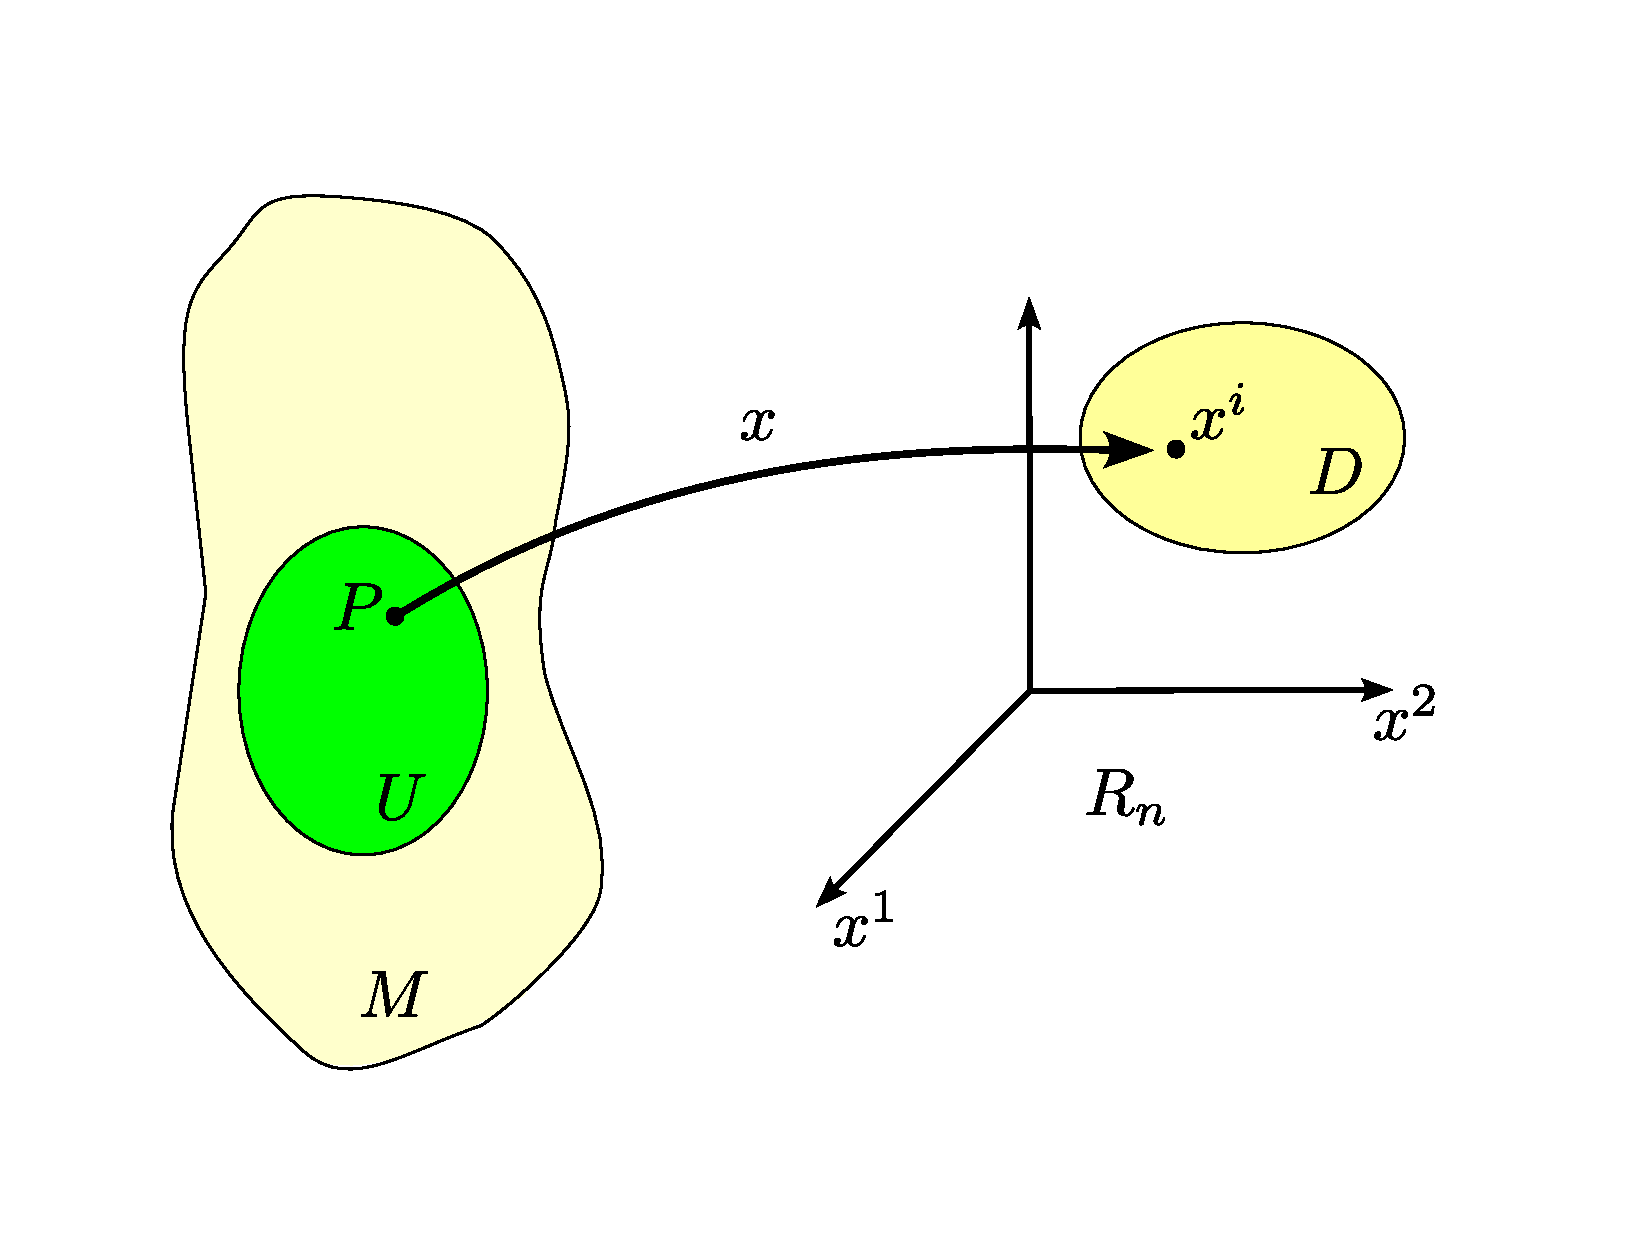
\includegraphics[height=6cm]{fig/fig-coordenadas.pdf}}
\caption{Una variedad y un sistema coordenado.}
\label{1-1}
\end{figure}
\end{center}

Como vemos en la figura \ref{1-1}, sobre cada vecindad $U$ pueden definirse sistemas coordenados (SC's) que asignan un'ivocamente a cada punto $P\in U$
un conjunto ordenado de n'umeros $x^i=(x^1,\dots ,x^n)$,
$i,j,\dots =1,\dots ,n$, llamados \textit{coordenadas de} $P$. Se exige que este mapeo uno a
uno sea continuo, de modo que, cuando $P$ se mueve en $U$, la correspondiente $n$-upla
($x^1,\dots ,x^n$) se mueve continuamente en un dominio $D$ contenido en $R_n$. Tambi'en se supone que la dimensi'on $n$ del mapeo de puntos de $M$ a $R_n$ es siempre la misma, en la vecindad de cada punto de la variedad.
\begin{center}
\begin{figure}[H]
\centerline{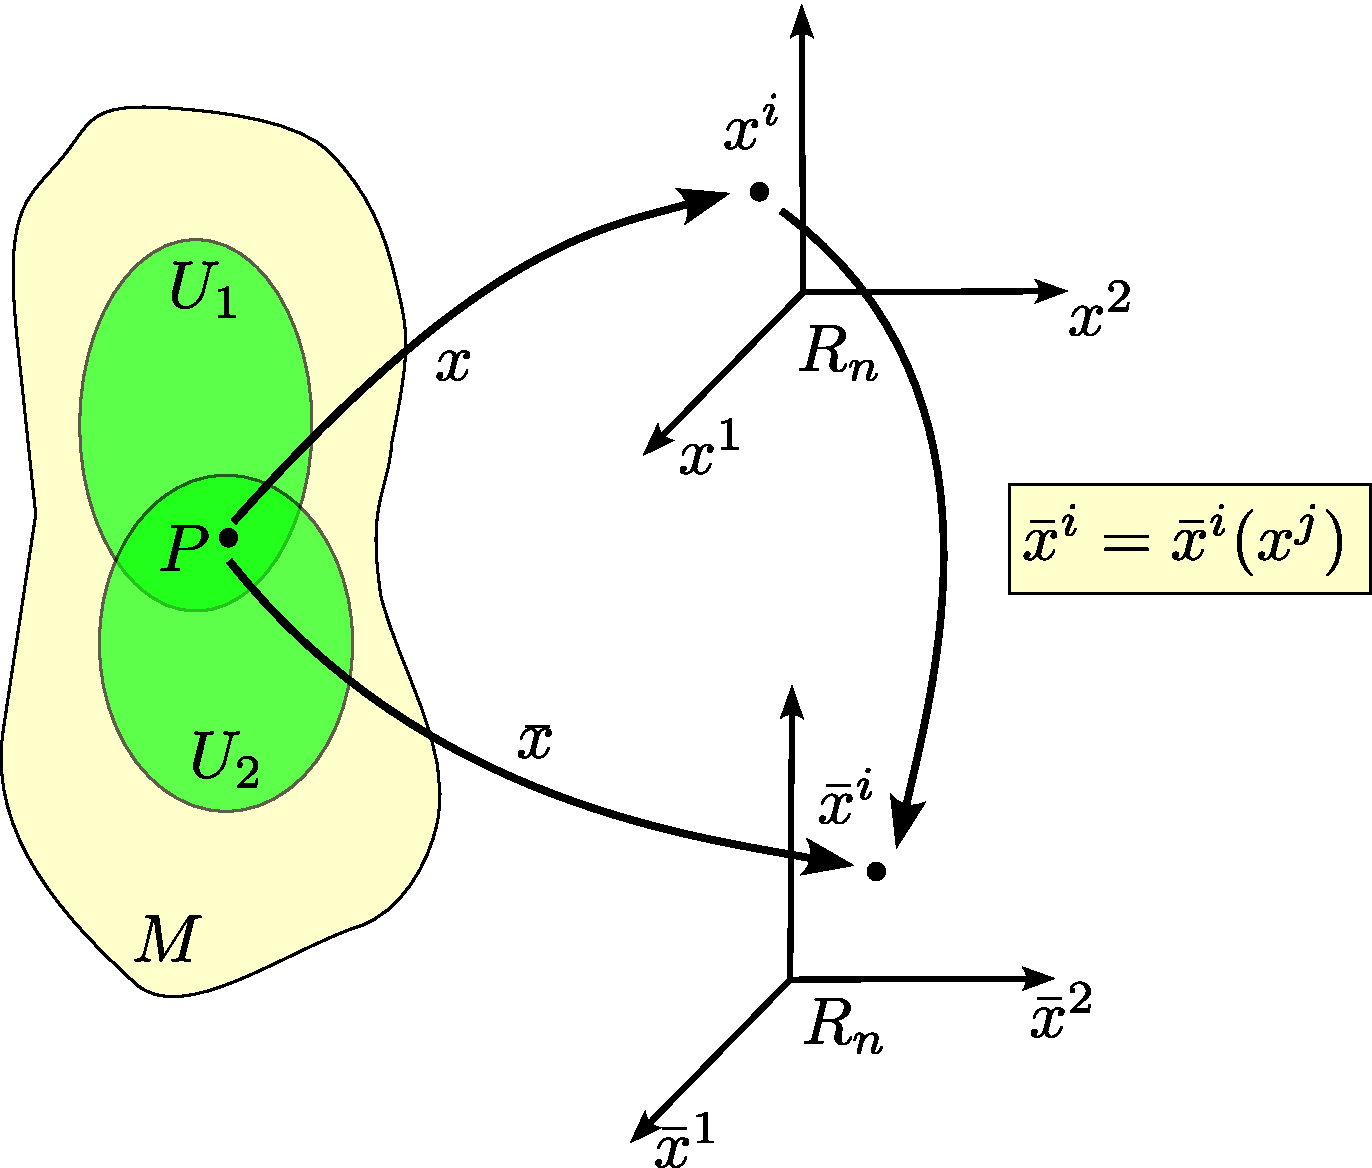
\includegraphics[height=6cm]{fig/fig-cambio-coordenadas.pdf}}
\caption{Una variedad y dos sistemas coordenados.}
\label{2-1}
\end{figure}
\end{center}

Consideremos la figura \ref{2-1}. El conjunto $M$ es una variedad diferenciable
si para cada punto $P$ en la
intersecci'on de dos abiertos, $U_1$, $U_2$ $\subseteq M$, los
correspondientes sistemas de coordenadas est'an relacionados por transformaciones diferenciables e invertibles: 
\begin{equation}
\bar{x}^j  =\bar{x}^j (x^i ), \qquad x^i  =x^i (\bar{x}^j ),\label{v1}
\end{equation}
de modo que, en cada punto de $U_1\cap U_2$,
\begin{equation}
\frac{\partial x^i }{\partial\bar{x}^j }\frac{\partial\bar{x}^j }{\partial
x^k }=\delta_k ^i, \qquad \frac{\partial\bar{x}^j }{\partial x^i 
}\frac{\partial x^i }{\partial\bar{x}^l }=\delta_l ^j , \label{v2}
\end{equation}
y adem'as
\begin{equation}
\frac{\partial(x^1,\dots ,x^n)}{\partial(\bar{x}^1
,\dots ,\bar{x}^n)}\cdot\frac{\partial(\bar{x}^1,\dots
,\bar{x}^n)}{\partial (x^1,\dots ,x^n)}=1. \label{v3}
\end{equation}

\section{Escalares, vectores y tensores}

En una variedad dada, es posible (y 'util) definir cantidades que representen magnitudes de inter'es f'isico. Estas cantidades pueden en general poseer componentes cuyos valores dependen del sistema de coordenadas usado para describir una cierta regi'on de la variedad. Por esto, es importante estudiar c'omo cambian las distintas cantidades definidas sobre una variedad bajo TGC's, clasific'andolas de acuerdo a la ley de transformaci'on que satisfacen. A continuaci'on estudiaremos la definici'on de vectores y tensores bajo TGC's. Note que los tensores no agotan todas las cantidades 'utiles de definir en una variedad\footnote{Por ejemplo, en algunas aplicaciones es 'util considerar objetos llamados \textbf{densidades tensoriales}, cuya ley de transformaci'on es distinta a los de los tensores. Adem'as, m'as adelante definiremos objetos llamados \textbf{conexiones}, que tampoco son tensores.}

\subsection{Escalares}
El caso m'as simple de una magnitud definida sobre una variedad es aquel en que se asocia un valor (real) a cada punto $P\in M$, el cual, por definici'on, no cambia bajo una transformaci'on de coordenadas (TC) arbitraria.

\begin{quotation}
\textbf{Definici'on:} Una cantidad real $\phi$, definido en un punto $P$ de la variedad $M$, es un \textbf{escalar} si bajo toda TGC se verifica que
\begin{equation}\marginnote{Escalar}
\boxed{\bar{\phi}(P)=\phi(P).} \label{t1}
\end{equation}
\end{quotation}

\subsection{Vectores contravariantes}

Consideremos dos puntos $P$ y $Q$, infinitesimalmente pr'oximos, de la variedad
$M$. Las respectivas coordenadas de estos puntos en un SC $x$ son
\begin{equation}
x^i(P)=x^i, \qquad x^i(Q)=x^i+dx^i.
\end{equation}
En otro SC $\bar{x}$, relacionado con el original por medio de (\ref{v1}),
tendremos
\begin{equation}
\bar{x}^i(P)=\bar{x}^i, \qquad \bar{x}^i(Q)=\bar{x}^i+d\bar{x}^i. \label{xP}
\end{equation}

Encontremos ahora la relaci'on entre las diferencias coordenadas $d\bar{x}^i$ y $dx^i$.
Usando (\ref{v1}) y (\ref{xP}b) podemos escribir
\begin{equation}
\bar{x}^i(Q)=\bar{x}^i(x(Q))=\bar{x}^i(x^j+dx^j)=\bar{x}^i(x^j)+\frac{
\partial\bar{x}^i}{\partial x^j}(x)dx^j,
\end{equation}
de modo que obtenemos
\begin{equation}\marginnote{Transf. de diferencias coordenadas}
\boxed{d\bar{x}^i_{P\rightarrow Q}=\frac{\partial\bar{x}^i}{\partial
x^j}(P)\,dx^j_{P\rightarrow Q}.} \label{tdx}
\end{equation}

Por tanto, bajo un cambio de SC, las diferencias de coordenadas entre puntos $P$ y
$Q$ infinitesimalmente pr'oximos cambian su valor, pero est'an relacionados por
medio del Jacobiano de la TGC, \textit{evaluado en el punto $P$}. La ley de
transformaci'on (\ref{tdx}) es el modelo para definir lo que llamaremos un
\textbf{vector contravariante}.

\begin{quotation}
\textbf{Definici'on:} Se dice que un conjunto de $n$ n'umeros
$A^i(P)=(A^1,\dots ,A^n)$, definidos en cada SC $x$, son las componentes  de un
\textbf{vector contravariante en un punto} $P$ (en el SC $x$), si bajo cada TGC (\ref{v1}), dichas componentes obedecen la siguiente ley de transformaci'on:
\begin{equation}\marginnote{Vector contravariante}
\boxed{\bar{A}^i(P)=\frac{\partial\bar{x}^i}{\partial x^j}(P)A^j(P).} \label{t9}
\end{equation}
\end{quotation}

De esta forma, la diferencia de coordenadas entre dos puntos infinitesimalmente pr'oximos $P$ y $Q$ define un vector contravariante infinitesimal en $P$. Equivalentemente, si $\cal C$ es una curva en $M$ (e.d. una subvariedad unidimensional de $M$), parametrizada (en una cierta vecindad y en alg'un SC definido en ella) por $x^i=x^i(\lambda)$ donde $\lambda$ es un par'ametro real continuo, entonces los \textbf{vectores tangentes} $A^ i(P):=(dx^i/d\lambda)(\lambda_P)$ son componentes de un vector contravariante asociado al punto $P$ (con coordenadas $x^i(P)=x^i(\lambda_P)$).

Se debe enfatizar que la ley de transformaci'on anterior define un vector
contravariante \textit{asociado a un punto dado} de la variedad. Esta identificaci'on de un vector con un punto de la variedad es necesaria ya que el jacobiano  ${\partial\bar{x}^i}/{\partial x^j}$ \textit{no es constante en general}, es decir, su valor depende del punto donde es evaluado. En general, cada punto de la variedad puede tener asociado infinitos vectores contravariantes. Es
f'acil comprobar que si $A^i(P)$ es un vector contravariante definido en un
punto $P$ dado, entonces $\alpha A^i(P)$ (donde $\alpha$ es un escalar) es un
nuevo vector contravariante en el punto $P$. An'alogamente, dado dos vectores
contravariantes $A^i(P)$ y $B^i(P)$ definidos \textit{en el mismo punto}
entonces $\alpha A^i(P)+\beta B^i(P)$ es tambi'en un vector contravariante en
$P$ (para valores arbitrarios de los escalares $\alpha$ y $\beta$). En otras
palabras, el conjunto de vectores contravariantes definidos \textit{en un mismo punto} $P$ define un \textbf{espacio vectorial $n$-dimensional}, que llamaremos \textbf{espacio tangente en $P$}: $T_n(P)$. \marginnote{Espacio Tangente}

Es importante destacar que los vectores contravariantes definidos en $P$ son
elementos del espacio tangente de $P$, y \textit{no son elementos de} $M$ (los
elementos de $M$ son los \textit{puntos} de la variedad). Note adem'as que las componentes $x^i$ de un punto $P$ de $M$ \textit{no son componentes de un vector} contravariante\marginnote{Coords. no son vectores bajo TGC's}, simplemente porque su ley de transformaci'on bajo TGC's es dada por (\ref{v1}), que es diferente de (\ref{t9})\footnote{Ambas leyes de transformaci'on, de las coordenadas y de vectores contravariantes, coinciden s'olo si restringimos nuestra atenci'on a transformaciones \textit{lineales} de coordenadas, de la forma $\bar{x}^i=L^i_{\ j}x^j$, donde $L^i_{\ j}$ son (en general 16 valores independientes) \textit{constantes}. Este hecho justifica porqu'e en mec'anica newtoniana y en la Teor'ia Especial de la Relatividad s'i es posible considerar las coordenadas como vectores, bajo rotaciones y transformaciones de Lorentz, respectivamente.}

\subsubsection{Representaci'on pict'orica de vectores contravariantes}
Es posible representar pict'oricamente un vector contravariante $A^i(P)$ por
medio de una ``flechita'' (infinitesimal) a partir del punto $P$. M'as detalladamente, dado un
vector contravariante $A^i(P)$ en $P$ es posible asociar consistentemente (esto quiere decir, independiente del SC usado) un punto $Q$ infinitesimalmente pr'oximo a $P$. En un SC dado (pero arbitrario) con coordenadas $x^i$, definimos las componentes del nuevo punto $Q$ por
\begin{equation}
x^i(Q):=x^i(P)+\varepsilon A^i(P), \label{defQ}
\end{equation}
donde $\varepsilon$ es un \textit{par'ametro escalar infinitesimal}.

La ley de transformaci'on de $A^i(P)$, es decir, el hecho 'este que sea un vector contravariante, asegura que la definici'on del punto $Q$ de la variedad por medio de (\ref{defQ}) sea independiente del SC usado. [En realidad, un vector contravariante define s'olo la \textit{direcci'on} de la correspondiente flechita, la ubicaci'on del punto $Q$ depende tambi'en del par'ametro infinitesimal $\varepsilon$].

Equivalentemente, es posible definir la representaci'on pict'orica de vectores contravariantes asoci'andoles una curva $\cal C$ (al menos, en alguna vecindad que incluya al punto $P$) tal que su vector tangente en $P$ sea igual (o proporcional, con una constante de proporcionalidad positiva) al vector $A^i(P)$, es decir, tal que $(dx^i/d\lambda)(P)=A^i(P)$.

\subsection{Vectores covariantes}

Consideremos un campo escalar $\phi$ definido en una regi'on de la variedad. En
un SC $x$ tendremos una dependencia expl'icita $\phi(x)$, y podemos calcular
las derivadas de $\phi$ respecto a las coordenadas $x^i$, es decir, el gradiente
del campo $\phi$, ${\partial \phi}/{\partial x^i}$, que define nuevos
campos. An'alogamente, si usamos un nuevo SC $\bar{x}$, tendremos otras
funciones expl'icitas $\phi(\bar{x})$ y podemos calcular el correspondiente
gradiente ${\partial \phi}/{\partial \bar{x}^i}$. En un punto $P$ dado,
podemos relacionar estos gradientes usando la transformaci'on coordenada
(\ref{v1}) y la regla de la cadena:
\begin{equation}
\boxed{\frac{\partial\phi}{\partial \bar{x}^i }(\bar{x}(P))=\frac{\partial x^j
}{\partial\bar{x}^i }(P)\frac{\partial\phi}{\partial x^j }(x(P)).} \label{tt2}
\end{equation}
Comparando (\ref{tt2}) con (\ref{t9}) vemos que las $n$ cantidades definidas por
\textit{el gradiente de un campo escalar} (calculado respecto a un SC) \textit{no forman
un vector contravariante}. En otras palabras, las derivadas de un campo escalar definen un nuevo tipo de objeto, que llamaremos \textbf{vector covariante}.

\begin{quotation}
\textbf{Definici'on:} Se dice que un conjunto de $n$ cantidades $A_i(P)=(A_1,\dots
,A_n)$ (definidas en cada SC) son las componentes (en el SC $x^i$) de un \textit{vector covariante en un punto} $P$, si bajo cada TGC (\ref{v1}) dichas componentes obedecen la siguiente ley de transformaci'on:
\begin{equation}\marginnote{Vector Contravariante}
\boxed{\bar{A}_i(P)=\frac{\partial x^j}{\partial\bar{x}^i}(P)A_j(P).}
\label{t6}
\end{equation}
\end{quotation}

An'alogamente al caso de vectores contravariantes, el conjunto de vectores
covariantes definidos en un punto dado $P$ de la variedad forma un espacio
vectorial $n$-dimensional: el \textbf{espacio cotangente en} $P$: $T_n^*(P)$. Es
importante notar que los espacios tangente y cotangente son espacios
vectoriales distintos definidos en cada punto de la variedad. Nuevamente, los
vectores covariantes son elementos del espacio cotangente de cada punto y no de la variedad $M$. Por otro lado, los vectores covariantes no pueden ser representados por ``flechitas'', ya que no est'an (directamente, al menos) relacionados con direcciones (desplazamientos) en la variedad.


\subsection{Tensores}
Consideremos el producto de las componentes $A^i (P)$ de un vector
contravariante y las componentes $B_j(P)$ de un vector covariante. Veamos
c'omo transforma el siguiente producto bajo una TGC:
\begin{equation}
\bar{A}^i (P)\bar{B}_j (P)=\frac{\partial\bar{x}^i }{\partial x^l }(P)A^l (P)
\frac{\partial x^k }{\partial\bar{x}^j }(P)B_k(P)=\frac{\partial\bar{x}^i 
}{\partial x^l }(P)\frac{\partial x^k }{\partial\bar{x}^j }(P)A^l (P)B_k(P).
\label{t11}
\end{equation}

Las $n^2$ cantidades $(A^i B_j)(P)$ transforman bajo una TCG en forma lineal y homog'enea seg'un la relaci'on (\ref{t11}). Esto motiva la siguiente definici'on:
\begin{quotation}
\textbf{Definici'on:} Un conjunto de $n^2$ cantidades $T_{\ j}^i (P)$ son las
componentes de un tensor de tipo $(^1_1)$ en un punto $P$, si bajo una TGC
dichas componentes transforman seg'un la ley:
\begin{equation}
\boxed{\bar{T}_{\ j}^i (P)=\frac{\partial\bar{x}^i }{\partial
x^k}(P)\frac{\partial x^l }{\partial\bar{x}^j}(P)\,T_{\ l}^k(P).} \label{t12}
\end{equation}
\end{quotation}

Note que en el ejemplo anterior, el tensor $T^i_{\ j}:=A^i B_j$ fue construido como un producto de las componentes de dos vectores (uno covariante y otro contravariante, en este caso). Sin embargo, \textit{no todo tensor de tipo $(^1_1)$ puede ser ``factorizado"\, en un producto de dos vectores}.

Podemos generalizar la definici'on anterior a objetos con m'as 'indices:
\begin{quotation}
\textbf{Definici'on:} Un conjunto de $n^{r+s}$ cantidades $T_{\ \ \ \ \ \
j_1\dots j_{s}}^{i_1\dots i_{r}}(P)$ son las componentes de un tensor de
rango $r+s$ y tipo $(^r_s)$ en un punto $P$ si, bajo cada TGC, dichas componentes
transforman seg'un la ley:
\begin{equation}\marginnote{Tensor general}
\boxed{\bar{T}_{\ \ \ \ \ \ \ j_1\cdots j_{s}}^{i_1\dots
i_{r}}(P)=\frac{\partial\bar{x}^{i_1}
}{\partial x^{k_1}}(P)\cdots \frac{\partial\bar{x}^{i_{r}}}{\partial
x^{k_{r}}}(P)\frac{\partial x^{l_1}}{\partial\bar{x}^{j_1}}(P)\cdots
\frac{\partial x^{l_{s}}}{\partial\bar{x}^{j_{s}}}(P)\,T_{\ \ \ \ \ \ \
l_1\cdots l_{s}}^{k_1\cdots k_{r}}(P).}
\label{t13}
\end{equation}
\end{quotation}
Note que $T_{\ \ \ \ \ \ \ j_1\dots j_s}^{i_1\dots i_r}(P)$ es un tensor de
car'acter mixto, contravariante de rango $r$ y covariante de rango $s$, definido en
el punto $P$.

Algunas consecuencias directas de la definici'on de tensores bajo TGC's son:
\begin{itemize}
\item Los dos tipos de vectores definidos previamente son casos
especiales de tensores. Un vector contravariante es un tensor del tipo
$(^1_0)$ y un vector covariante es un tensor del tipo $(^0_1)$. Un
escalar puede ser considerado como un tensor de tipo $(^0_0)$.

\item La relaci'on (\ref{v2}b) puede ser escrita en la forma:
\begin{equation}
\delta_l ^j =\frac{\partial\bar{x}^j }{\partial x^i }(P)\frac{\partial
x^k }{\partial\bar{x}^l }(P)\,\delta_k ^i , \label{t15}
\end{equation}
lo cual muestra que (los $n^2$ n'umeros definidos por) la delta de Kronecker
define un tensor del tipo $(^1_1)$. Adem'as, la delta de Kronecker es una de las muy pocas entidades tensoriales \textit{num'ericamente invariantes} (es decir, que asume los mismos valores en todo SC) que es posible definir en una variedad cualquiera.

\item Una de las caracter'isticas principales de los tensores es que si
todas las componentes de un tensor son nulas en un SC entonces ellas se anulan
\textit{en todo SC}. Esto se verifica directamente a partir de (\ref{t13}) y en
particular del hecho que la transformaci'on es \textit{homog'enea}\footnote{Los tensores no son los 'unicos objetos 'utiles que cumplen esta propiedad, las \textbf{densidades tensoriales} tambi'en lo hacen.}.
\end{itemize}

\section{Algebra tensorial sobre variedades diferenciables}

Dadas las componentes de uno o m'as tensores, es posible definir una infinidad de operaciones algebraicas usando sus componentes. Sin embargo, s'olo algunas de estas operaciones definir'an nuevos tensores. A continuaci'on resumiremos las operaciones algebraicas b'asicas (m'as usadas) que mapean tensores en tensores (no necesariamente del mismo tipo).


\subsection{Multiplicaci'on}

La multiplicaci'on de todas las componentes de un tipo ($_{s_1}^{r_1}$) con las de otro de tipo ($_{s_2}^{r_2}$), definidos en un mismo punto $P$, conduce a un tensor de
tipo ($_{s_1+s_2}^{r_1+r_2}$) en $P$. Este proceso es llamado
\textbf{producto directo}.

Para ilustrar esto consideramos, por ejemplo, un tensor de tipo ($_1^2$) y
un tensor de tipo ($_2^0$), pues el razonamiento es general. Sus leyes de
transformaci'on son, respectivamente\footnote{Desde ahora, para no recargar la notaci'on, omitiremos el punto $P$ donde cada tensor es definido.}:
\begin{align}
\bar{T}_{\ \ m}^{jl} & =\frac{\partial\bar{x}^j }{\partial x^i }\frac
{\partial\bar{x}^l }{\partial x^k }\frac{\partial x^p}{\partial\bar{x}
^m }\,T_{\ \ p}^{ik},\label{mul1}\\
\bar{S}_{qr} & =\frac{\partial x^{t}}{\partial\bar{x}^q}\frac{\partial
x^{u}}{\partial\bar{x}^r}\,S_{tu}.\nonumber
\end{align}
El producto de las componentes de estos dos tensores se transforma de acuerdo a:
\begin{equation}
\bar{T}_{\ \ m}^{jl}\bar{S}_{qr}=\frac{\partial\bar{x}^j }{\partial x^i
}\frac{\partial\bar{x}^l}{\partial x^k}\frac{\partial
x^p}{\partial\bar{x}^m}
\frac{\partial x^t}{\partial\bar{x}^q}\frac{\partial
x^{u}}{\partial\bar{x}^r}\,T_{\ \ p}^{ik}S_{tu}, \label{2}
\end{equation}
que es la ley de transformaci'on de las componentes de un
tensor de tipo $(^3_2)$, $V_{\ \ klm}^{ij}:=T_{\ \ k}^{ij}S_{lm}$. Note que esta conclusi'on es v'alida s'olo si ambos tensores $T$ y $S$ est'an \textit{definidos en el mismo punto}.

Como caso particular vemos que la multiplicaci'on de (todas) las componentes de
un tensor de tipo $(^r_s)$ por un escalar (es decir, un tensor de tipo $(^0_0)$ conduce a un tensor del mismo tipo.

\subsection{Adici'on}

Sea $S_{\ \ \ \ \ \ k_1\dots k_{s}}^{i_1\dots i_{r}}$ un tensor del
tipo $(^r_s)$ definido en el punto $P$. Su ley de transformaci'on, de acuerdo
con
(\ref{t13}), es:
\begin{equation}
\bar{S}_{\ \ \ \ \ \ k_1\dots k_{s}}^{i_1\dots
i_{r}}=\frac{\partial\bar{x}^{i_1}
}{\partial x^{l_1}}\dots \frac{\partial\bar{x}^{i_{r}}}{\partial x^{l_{r}}
}\frac{\partial x^{m_1}}{\partial\bar{x}^{k_1}}\dots \frac{\partial x^{m_{s}
}}{\partial\bar{x}^{k_{s}}}\,S_{\ \ \ \ \ \ m_1\dots m_{s}}^{l_1\dots
l_{r}},
\label{ad1}
\end{equation}
y sea el tensor $T_{\ \ \ \ \ \ k_1\dots k_{s}}^{i_1\dots i_{r}}$ otro
tensor de tipo $(^r_s)$, entonces la suma de sus componentes $T_{\ \ \ \ \ \
k_1\dots k_{s}}^{i_1\dots i_{r}}+S_{\ \ \ \ \ \ k_1\dots
k_{s}}^{i_1\dots i_{r}}$ definen un nuevo tensor de tipo $(^r_s)$ ya que
\begin{equation}
\bar{T}_{\ \ \ \ \ \ k_1\dots k_{s}}^{i_1\dots i_{r}}+\bar{S}_{\ \ \ \ \ \
k_1\dots k_{s}}^{i_1\dots i_{r}}=\frac{\partial\bar{x}^{i_1}}{\partial
x^{l_1}}\dots \frac{\partial\bar{x}^{i_{r}}}{\partial x^{l_{r}}}\frac{\partial
x^{m_1}}{\partial\bar{x}^{k_1}}\dots
\frac{\partial x^{m_{s}}}{\partial\bar{x}^{k_{s}}}\left( T_{\ \ \ \ \ \
m_1\dots m_{s}}^{l_1\dots l_{r}}+S_{\ \ \ \ \ \ m_1\dots
m_{s}}^{l_1\dots l_{r}}\right) .\label{ad2}
\end{equation}

La operaci'on de multiplicaci'on puede ser combinada con la de adici'on de tensores, 
siempre que sus respectivos tipos sean apropiados. Estas operaciones satisfacen las leyes conmutativa, asociativa y distributiva.

Combinando la adici'on con la multiplicaci'on por escalar vemos que el conjunto de todos los tensores de un tipo $(^r_s)$ dado, en el punto $P$ de $M$, constituye un espacio vectorial de dimensi'on $n^{r+s}$.

Es importante notar que una combinaci'on lineal de tensores de \textit{distinto
tipo} en un mismo punto, o de tensores del mismo tipo, pero \textit{en distintos puntos},
 \textit{no suministra un nuevo tensor}.


\subsection{Contracci'on}

Dado un tensor de tipo $(^r_s)$ es posible construir un tensor de tipo
($_{s-1}^{r-1}$) seleccionando un super'indice y un sub'indice y
sumando sobre componentes iguales, de acuerdo con la convenci'on de suma de
Einstein. En efecto, de (\ref{t13}) obtenemos que si sumamos sobre el $p$-'esimo indice contravariante y el $q$-'esimo covariante, tendremos que
\begin{eqnarray}
\bar{T}_{\ \ \ \ \ \ \ \ \ k_1\cdots i\cdots k_{s}}^{i_1\cdots i\cdots
i_{r}}
&=&\frac{\partial\bar{x}^{i_1}}{\partial x^{l_1}}\cdots
\frac{\partial\bar{x}^{i_{p-1}}}{\partial x^{l_{p-1}}}\,\frac{\partial\bar{x}^i}{\partial x^l}\,\frac{\partial\bar{x}^{i_{p+1}}}{\partial x^{l_{p+1}}}\cdots \frac{\partial\bar{x}^{i_{r}}}{\partial x^{l_{r}}}
 \nonumber \\
&& \times\ \frac{\partial x^{m_1}}{\partial\bar{x}^{k_1}}\frac{\partial x^{m_{q-1}}}{\partial\bar{x}^{k_{q-1}}}\frac{\partial x^{m}
}{\partial\bar{x}^i }\frac{\partial x^{m_{q+1}}}{\partial\bar{x}^{k_{q+1}}}\cdots
\frac{\partial x^{m_{s}}}{\partial\bar{x}^{k_{s}}}\,T_{\ \ \ \ \ \ \ \ \
m_1\cdots m\cdots m_{s}}^{l_1\cdots l\cdots l_{r}} \label{con1}\\
&=&\left(\frac{\partial\bar{x}^i }{\partial x^l }\frac{\partial x^m
}{\partial\bar{x}^i }\right)\frac{\partial\bar{x}^{i_1}}{\partial x^{l_1}}\cdots
\frac{\partial\bar{x}^{i_{p-1}}}{\partial
x^{l_{p-1}}}\frac{\partial\bar{x}^{i_{p+1}}}{\partial
x^{l_{p+1}}}\cdots\frac{\partial\bar{x}^{i_{r}}}{\partial x^{l_{r}}}\nonumber \\
&& \times\ \frac{\partial x^{m_1}}{\partial\bar{x}^{k_1}}\frac{\partial x^{m_{q-1}}}{\partial\bar{x}^{k_{q-1}}} \frac{\partial
x^{m_{q+1}}}{\partial\bar{x}^{k_{q+1}}}\cdots \frac{\partial x^{m_{s}}}
{\partial\bar{x}^{k_{s}}}\,T_{\ \ \ \ \ \ \ \ \ m_1\cdots m\cdots
m_{s}}^{l_1\cdots l\cdots l_{r}}\\
&=&\delta_l ^m\, \frac{\partial\bar{x}^{i_1}}{\partial x^{l_1}}\cdots
\frac{\partial\bar{x}^{i_{p-1}}}{\partial
x^{l_{p-1}}}\frac{\partial\bar{x}^{i_{p+1}}}{\partial
x^{l_{p+1}}}\cdots\frac{\partial\bar{x}^{i_{r}}}{\partial x^{l_{r}}}\nonumber \\
&& \times\ \frac{\partial x^{m_1}}{\partial\bar{x}^{k_1}}\frac{\partial x^{m_{q-1}}}{\partial\bar{x}^{k_{q-1}}} \frac{\partial
x^{m_{q+1}}}{\partial\bar{x}^{k_{q+1}}}\cdots \frac{\partial x^{m_{s}}}
{\partial\bar{x}^{k_{s}}}\,T_{\ \ \ \ \ \ \ \ \ m_1\cdots m\cdots
m_{s}}^{l_1\cdots l\cdots l_{r}}\\
&=&\underbrace{\frac{\partial\bar{x}^{i_1}}{\partial x^{l_1}}\cdots
\frac{\partial\bar{x}^{i_{p-1}}}{\partial x^{l_{p-1}}} \frac{\partial\bar{x}^{i_{p+1}}}{\partial x^{l_{p+1}}} \cdots\frac{\partial\bar{x}^{i_{r}}}{\partial x^{l_{r}}}}_{(r-1) \text{
t'erminos}}\nonumber \\
&& \times \underbrace{\frac{\partial
x^{m_1}}{\partial\bar{x}^{k_1}}\frac{\partial
x^{m_{q-1}}}{\partial\bar{x}^{k_{q-1}}} \frac{\partial
x^{m_{q+1}}}{\partial\bar{x}^{k_{q+1}}}\cdots \frac{\partial x^{m_{s}}}
{\partial\bar{x}^{k_{s}}}}_{(s-1) \text{ t'erminos}}\,T_{\ \ \ \ \ \ \ \ \
m_1\cdots l\cdots m_{s}}^{l_1\cdots l\cdots l_{r}}.
\end{eqnarray}
Por tanto, $T_{\ \ \ \ \ \ \ \ \ k_1\dots i\dots k_{s}}^{i_1\dots i\dots
i_{r}} $ satisface ley de transformaci'on de un tensor de tipo ($_{s-1}^{r-1}$).
Este proceso es conocido como \textbf{contracci'on}.

Claramente, el proceso de contracci'on de un tensor de tipo ($_1^1$) da
origen a un escalar. En particular, para el caso de la delta de Kronecker
tenemos:
\begin{equation}
\delta_j^j =\delta_1^1+\dots \delta_n^n=n. \label{con2}
\end{equation}


\subsection{Permutaci'on y (Anti-)Simetrizaci'on}

Es directo verificar que la \textit{permutaci'on de dos 'indices del mismo tipo (covariante o contravariante)} de un tensor define un nuevo tensor. Por ejemplo, si $A_{ij}$ son las componentes de un tensor de tipo $(^0_2)$ entonces las nuevas componentes $B_{ij}$ determinadas por la permutaci'on de las componentes de $A_{ij}$, es decir, $B_{ij}:=A_{ji}$ tambi'en son las componentes de un tensor del mismo tipo. Lo mismo ocurre si se permutan dos 'indices contravariantes. Sin embargo, \textit{esto no ocurre si se permutan 'indices de distinto tipo}\footnote{Por ejemplo, si a partir de $A^i_{\ j}$ se define $B^i_{\ j}:=A^j_{\ i}$ o, m'as expl'icitamente, $B^1_{\ 2}:=A^2_{\ 1}$, $B^2_{\ 3}:=A^3_{\ 2}$, etc.}.

 Un tensor es llamado \textit{sim'etrico} con respecto a un par de 'indices (del mismo tipo, ya sean covariantes o contravariantes) si una permutaci'on de ellos no afecta el valor de las componentes de dicho tensor. Si, por otro lado, este proceso afecta a cada
componente multiplic'andola por $-1$, entonces el tensor es llamado
\textit{antisim'etrico} en dichos 'indices. Finalmente, se dice que un tensor es
\textit{totalmente (anti-)sim'etrico} si lo es con todo a cualquier de 'indices. En general, cuando hablemos de tensores (anti-)sim'etricos nos referimos a tensores totalmente (anti-)sim'etricos, salvo que se indique lo contrario.

Por ejemplo, si $A_{ij}$ y $B_{ij}$ son las componentes de tensores de tipo
($_2^0$), entonces $A_{ij}$ es un tensor sim'etrico si:
\begin{equation}
A_{ij}=A_{ji}, \label{sim1}
\end{equation}
y $B_{ij}$ ser'a un tensor antisim'etrico si
\begin{equation}
B_{ij}=-B_{ji}. \label{sim2}
\end{equation}

Como consecuencia inmediata de la forma de la ley de transformaci'on de
tensores, estas ecuaciones son v'alidas en cualquier sistema coordenado.

\begin{quotation}
\textbf{Teorema:} \textit{Todas las propiedades de simetr'ia y de
antisimetr'ia de los tensores (respecto a 'indices del mismo tipo) son independientes de la elecci'on del sistema coordenado.}
\end{quotation}

Dado un tensor de tipo $(^r_s)$ con $r>1$ 'o $s>1$, podemos construir
a partir de dicho tensor, un tensor sim'etrico y un tensor
antisim'etrico respecto a cualquier par de 'indices del mismo tipo. Por ejemplo, a partir del tensor $A_{ij}$ podemos definir los nuevos tensores
\begin{align}
A_{(ij)} & :=\frac{1}2\left( A_{ij}+A_{ji}\right) ,\label{sim3}\\
A_{[ij]} & :=\frac{1}2\left( A_{ij}-A_{ji}\right) ,\nonumber
\end{align}
que son sim'etricos y antisim'etricos, respectivamente. El proceso
correspondiente a definir $A_{(ij)}$ a partir de $A_{ij}$ es llamado \textbf{simetrizaci'on}. An'alogamente $A_{[ij]}$ resulta del proceso de \textbf{antisimetrizaci'on}.

Vemos tambi'en que todo tensor de tipo $(^r_s)$ con $r>1$ 'o $s>1$, se
puede expresar como suma de un tensor sim'etrico y uno antisim'etrico respecto a
cualquier par de 'indices del mismo tipo. En el caso anterior
tenemos:
\begin{equation}
A_{ij}=A_{(ij)}+A_{[ij]}.\label{sim4}
\end{equation}

Es posible extender el proceso de (anti-)simetrizaci'on a m'as de dos 'indices, por
medio de
\begin{eqnarray}
T_{[ij]}&:=&\frac{1}2(T_{ij}-T_{ji}), \\
T_{[ijk]}&:=&\frac{1}{3}(T_{i[jk]}+T_{j[ki]}+T_{k[ij]}), \label{as3}\\
T_{[ijkl]}&:=&\frac{1}{4}(T_{i[jkl]}-T_{j[kli]}+T_{k[lij]}-T_{l[ijk]}),
\end{eqnarray}
etc'etera, y
\begin{eqnarray}
T_{(ij)}&:=&\frac{1}2(T_{ij}+T_{ji}), \\
T_{(ijk)}&:=&\frac{1}{3}(T_{i(jk)}+T_{j(ki)}+T_{k(ij)}), \\
T_{(ijkl)}&:=&\frac{1}{4}(T_{i(jkl)}+T_{j(kli)}+T_{k(lij)}+T_{l(ijk)}),
\end{eqnarray}
etc'etera.

\subsection{Invariancia de las ecuaciones tensoriales}

Hemos visto que los tensores pueden ser sumados, restados o, m'as
generalmente, linealmente combinados con coeficientes escalares. Podemos
formar productos entre tensores y/o contraerlos, definiendo nuevos tensores, siempre
que  ellos est'en definidos en el mismo punto de $M$. Todas estas operaciones suministran nuevos tensores.

Un importante tensor de cada tipo es el \textbf{tensor
nulo} de ese tipo. Dicho tensor es num'ericamente invariante debido a que la ley de transformaci'on de tensores es \textit{homog'enea}. Esto tiene
como consecuencia que una ecuaci'on tensorial como
$S_{\ \ \ \ kl\cdots }^{ij\cdots }=T_{\ \ \ \ kl\cdots }^{ij\cdots }$ sea
v'alida \textit{con la misma forma} en todo sistema coordenado, ya que es equivalente a afirmar que $S_{\
\ \ \ kl\cdots }^{ij\cdots }-T_{\ \ \ \ kl\cdots }^{ij\cdots }$ es el tensor
nulo.
Este hecho garantiza adem'as el teorema de la invariancia de las propiedades de
simetr'ia y antisimetr'ia de los tensores. Si $S$ y $T$ son de distinto tipo, o
bien, si est'an definidos en puntos distintos, la ecuaci'on carece de sentido
invariante (independiente de las coordenadas usadas).

% Consideremos ahora un tensor de tipo $(_{s}^r)$, $r$ vectores covariantes,
% $s$ vectores contravariantes, y el siguiente producto contra'ido:
% \begin{equation}
% S_{\ \ \ \ pq\dots }^{kl\dots }A_k B_l \cdots F^pG^q\cdots .
%\label{inv1}%
% \end{equation}
%
%
% Entonces, de acuerdo con las reglas de producto externo e interno, esta
% multiplicaci'on es un escalar. La proposici'on inversa es tambi'en verdadera:
%Supongamos que no sabemos si un arreglo de n'umeros $S_{\ \ \ \ \dots
%}^{\dots }$ tiene caracter tensorial, pero
% sabemos que (\ref{inv1}) es un escalar para cualquier conjunto arbitrario de
% vectores $A\cdots G\cdots $. Entonces $S_{\ \ \dots }^{\dots }$ son las
%componentes de un tensor
% del tipo definido por sus 'indices.
%
% En efecto, para probar esto consideremos una transformaci'on particular y
% llamemos $\bar{S}_{\ \ \dots }^{\dots }$ a las componentes de $S$
%transformadas como si
% fuera un tensor. Llamemos $\tilde{S}_{\ \ \dots }^{\dots }$ a cualquier
%conjunto de
% n'umeros que comparte con $\bar{S}_{\ \ \dots }^{\dots }$ la propiedad de
%hacer
% (\ref{inv1}) un escalar. Entonces tenemos que
% \begin{align}
% \bar{S}_{\ \ \ \ pq\dots }^{kl\dots }\bar{A}_k \bar{B}_l \cdots
%\bar{F}^p\bar{G}^q\cdots  &=S_{\ \ \ \ pq\dots }^{kl\dots }A_k B_l \cdots
%F^pG^q\cdots , \label{inv2}\\
% \tilde{S}_{\ \ \ \ pq\dots }^{kl\dots }\bar{A}_k \bar{B}_l \cdots
%\bar{F}^p\bar{G}^q\cdots
% & =S_{\ \ \ \ pq\dots }^{kl\dots }A_k B_l \cdots F^pG^q\cdots .
% \end{align}
% Estas ecuaciones expresan que $\bar{S}_{\ \ \dots }^{\dots }$ y $\tilde{S}_{\
%\ \dots }^{\dots }$
% dejan (\ref{inv1}) invariante. Rest'andolas obtenemos:
% \begin{equation}
% \left( \bar{S}_{\ \ \ \ pq\dots }^{kl\dots }-\tilde{S}_{\ \ \ \ pq\dots
%}^{kl\dots }\right) \bar{A}%
% _k \bar{B}_l \dots \bar{F}^p\bar{G}^q\dots  =0 .\label{inv3}
% \end{equation}
% Usando el supuesto que los vectores $A\cdots G\dots $ son arbitrarios,
%encontramos que
% \begin{equation}
% \bar{S}_{\ \ \ \ pq\dots }^{kl\dots }-\tilde{S}_{\ \ \ \ pq\dots }^{kl\dots }
%=0,
% \end{equation}
% es decir, que los tensores $\bar{S}$ y $\tilde{S}$ son iguales:
% \begin{equation}
% \bar{S}_{\ \ \ \ pq\dots }^{kl\dots }  =\tilde{S}_{\ \ \ \ pq\dots }^{kl\dots
%}.
% \end{equation}
% Por lo tanto, bajo las hip'otesis mencionadas $S$ debe ser un tensor.

 \section{Densidades tensoriales *}

 Consideremos un campo vectorial contravariante $A^i $ y la integral:
 \begin{equation}
 \int_\Omega A^i d^nx, \label{den1}%
 \end{equation}
 donde $d^nx:=dx^1dx^2\cdots dx^n$ y la integral se toma sobre una
 regi'on $\Omega$ dada de $M$. Observamos que el resultado de esta integral
 \textit{no constituye un vector bajo TGC's} (ya que b'asicamente se est'an
 sumando vectores definimos en distintos puntos de la variedad, que bajo una
 TGC transforman de forma distinta en cada punto). Del mismo modo,
 consideremos la integral de un campo escalar $A$:
 \begin{equation}
 I=\int_\Omega A\,d^nx. \label{den2}%
 \end{equation}
 Veamos c'omo transforma bajo $I$ bajo una TGC. El elemento de volumen
 transforma de acuerdo al teorema de cambio de variables para integrales de
 Riemann m'ultiples:
 \begin{equation}
 d^nx=\left| \frac{\partial x^k }{\partial\bar{x}^j }\right| d^n
 \bar{x} ,
 \end{equation}
 donde $\left| \frac{\partial x^k }{\partial\bar{x}^j }\right|$ es el m'odulo
 del jacobiano de la transformaci'on. Luego:
 \begin{equation}
 I=\int_\Omega A\,d^nx=\int_\Omega\bar{A}\left| \frac{\partial x^k
 }{\partial\bar{x}^j %
 }\right| d^n\bar{x}\neq\int_\Omega\bar{A}\,d^n\bar{x}=\bar{I}.
 \label{den3}%
 \end{equation}
 De este modo $I$ \textit{no es invariante bajo una TGC} (de hecho, $I$ y
 $\bar{I}$ ni siquiera son proporcionales, en general). Pero nos interesa poder
 definir integrales de la forma (\ref{den2}) cuyo resultado s'i sea un
 escalar, es decir, independiente del SC en el que se calcule. Esto implica
 entonces que, para que $I$ sea un escalar, $A$ no puede ser un campo escalar.
 Por otra parte,
 sabemos que si sumamos s'olo cantidades escalares el resultado es un escalar.
 En nuestro caso tenemos una integral en vez de una suma. Luego, si
 $A\,d^nx$ es
 un escalar entonces $I$ ser'a un escalar. Para esto la ley de transformaci'on
 de $A$ no debe ser $A=\bar{A}$, sino\footnote{Desde ahora, denotaremos a las
 densidades (tensoriales) usando letras cursivas.}
 \begin{equation}
 {\cal A}=\left| \frac{\partial\bar{x}^i }{\partial x^k }\right| \bar{{\cal
 A}},
 \label{den4}%
 \end{equation}
 de modo que
 \begin{equation}
 I=\int_\Omega {\cal A}\,d^nx=\int_\Omega\bar{{\cal A}}\left|
 \frac{\partial\bar{x}^i }{\partial x^k %
 }\right| \left| \frac{\partial x^k }{\partial\bar{x}^j }\right|
 d^n\bar{x}
 =\int_\Omega\bar{{\cal A}}\,d^n\bar{x}=\bar{I}. \label{den5}%
 \end{equation}
 Ahora $I$ es un escalar, pero ${\cal A}$ no lo es. Esto motiva la siguiente
 definici'on:

 \textbf{Definici'on:} Una cantidad $\rho$ es llamada \textit{densidad escalar
 de peso} $p$ si bajo una TGC 'esta obdece la ley:
 \begin{equation}
 \bar{\rho}=\left| \frac{\partial x^i }{\partial\bar{x}^j }\right| ^p%
 \rho. \label{den6}%
 \end{equation}
 De lo anterior se concluye que $d^nx$ es una densidad escalar de peso $-1$,
 y que la integral de una densidad escalar de peso $+1$ es un escalar.

 \textbf{Definici'on:} Un conjunto de $n^{r+s}$ cantidades ${\cal A}_{\ \ \ \ \
 k_1\cdots k_{s}}^{i_1\cdots i_{r}}(P)$ son las componentes de una densidad
 tensorial de peso $p$ y tipo $(^r_s)$ en un punto $P$, si bajo una TGC dichas
 componentes transforman seg'un la ley:
 \begin{equation}
 \boxed{\bar{{\cal A}}_{\ \ \ \ \ k_1\cdots k_{s}}^{i_1\cdots
 i_{r}}(P)=\left| \frac{\partial
 x^i }{\partial\bar{x}^k }\right|^p(P) \frac{\partial\bar{x}^{i_1}%
 }{\partial x^{l_1}}(P)\cdots \frac{\partial\bar{x}^{i_{r}}}{\partial
 x^{l_{r}}}(P)\frac{\partial x^{m_1}}{\partial\bar{x}^{k_1}}(P)\cdots
 \frac{\partial x^{m_{s}}}{\partial\bar{x}^{k_{s}}}(P){\cal A}_{\ \ \ \ \
 m_1\cdots m_{s}}^{l_1\cdots l_{r}}(P).}
 \label{den7}%
 \end{equation}
 No se debe inferir que la integral de las componentes de una densidad
 tensorial es un tensor, pues no lo es (salvo el caso de una densidad escalar).

 Consecuencias inmediatas de la definici'on de densidades tensoriales son:
 \begin{itemize}
 \item Si todas las componentes de una densidad son nulas en un SC, entonces
 son nulas en cualquier SC. Como consecuencia, las ecuaciones entre densidades
 son independientes del SC.
 \item La suma o diferencia de densidades del mismo tipo y referidas al mismo
 punto es otra densidad del mismo tipo.
 \item El producto de una densidad tensorial de tipo $(^r_s)$ y peso $p$ por
 una densidad tensorial de tipo $(^t_u)$ y peso $q$ es una densidad tensorial
 de tipo $(^{r+t}_{s+u})$ y peso $p+q$.
 \item La contracci'on de 'indices puede realizarse para densidades
 tensoriales de tipo $(^r_s)$ con $r,s\geq1$, del mismo modo que para tensores,
 resultando una densidad de tipo ($_{s-1}^{r-1}$) y del mismo peso.
 \end{itemize}

 \subsection{Densidades tensoriales de Levi-Civita*}
 Considere ahora un tensor $T_{i_1\cdots i_n}$ de tipo ($_n^0$)
 \textit{totalmente
 antisim'etrico}. Si denotamos el valor num'erico de $T_{12\dots n}$ por
 ${\cal T}$, entonces cualquier otra componente $T_{i_1\cdots i_n}$ tendr'a
 valor
 $\pm{\cal T}$ de acuerdo a si la permutaci'on $i_1\cdots i_n$ es par o
 impar, o
 bien ser'a nula si se repite un 'indice. Escribamos la ley de transformaci'on
 para la componente $T_{12\cdots n}$:
 \begin{equation}
 \bar{T}_{12\cdots n}=\frac{\partial
 x^{k_1}}{\partial\bar{x}^1}\frac{\partial
 x^{k_2}}{\partial\bar{x}^2}\cdots \frac{\partial x^{k_n}}{\partial\bar
 {x}^n}\,T_{k_1\cdots k_n}. \label{den8}%
 \end{equation}
 Escribiendo expl'icitamente la suma y usando las propiedades
 antisim'etricas de $T$ se obtiene:
 \begin{equation}
 \bar{T}_{12\cdots n}=\left| \frac{\partial x^k }{\partial\bar{x}^i }\right|
 T_{12\cdots n}, \label{den9}%
 \end{equation}
 es decir,
 \begin{equation}
 \bar{{\cal T}}=\left| \frac{\partial x^k }{\partial\bar{x}^i }\right| {\cal
 T}.
 \label{den10}%
 \end{equation}
 Esto significa que el valor de una componente (no nula) de un tensor
 antisim'etrico de tipo ($_n^0$) es una densidad escalar de tipo $+1$. Por
 otro lado, ya que todos los valores de $T_{i_1\cdots i_n}$ son
 proporcionales a $T_{12\cdots n}={\cal T}$, podemos escribir que
 \begin{equation}
 T_{i_1\cdots i_n}={\cal T}\hat{\epsilon}_{i_1\cdots i_n},
 \label{TcalT}
 \end{equation}
 donde $\hat{\epsilon}_{i_1\cdots i_n}$ denota un objeto que es definido
 tal que es totalmente antisim'etrico y que \textit{en todo SC}
 $\hat{\epsilon}_{12\cdots n}:=1$. Ya que $T_{i_1\cdots i_n}$ es un tensor
 (es decir, una densidad tensorial de peso $0$) y ${\cal T}$ es una densidad
 tensorial de peso $+1$ concluimos de (\ref{TcalT}) que
 $\hat{\epsilon}_{i_1\cdots i_n}$ \textbf{es una densidad tensorial de
 peso} $-1$, llamada \textbf{densidad tensorial de Levi-Civita}.

 An'alogamente, podemos descomponer cualquier tensor contravariante
 $A^{i_1\cdots i_n}$ en
 \begin{equation}
 A^{i_1\cdots i_n}={\cal A}\,\epsilon^{i_1\cdots i_n}, \label{AcalA}
 \end{equation}
 donde ${\cal A}:=A^{1\cdots n}$ es una densidad escalar de peso $-1$ y
 $\epsilon^{i_1\cdots i_n}$ es la densidad de Levi-Civita de peso $+1$,
 definida como totalmente antisim'etrica y tal que
 \textit{en todo SC} $\epsilon^{1\cdots n}:=1$.

 Las densidades tensoriales de Levi-Civita son cantidades num'ericamente
 invariantes que pueden ser definidas en cualquier variedad.


 En el caso que $n=4$, ellas satisfacen las siguientes identidades:
 \begin{eqnarray}
 \epsilon^{ijkl}\, \hat{\epsilon}_{mnpq}&=&4!\, \delta^i_{[m}\delta ^j_n
 \delta^k_p \delta^l_{q]}, \\
 \epsilon^{ijkl}\, \hat{\epsilon}_{mnpl}&=&3!\, \delta^i_{[m}\delta ^j_n
 \delta^k_{p]} , \\
 \epsilon^{ijkl}\, \hat{\epsilon}_{mnkl}&=&2!\, \left( \delta^i_m\delta ^j_n -
 \delta^j_m \delta^i_n\right), \label{idep2} \\
 \epsilon^{ijkl}\, \hat{\epsilon}_{mjkl}&=&3!\, \delta^i_m, \label{idep3}\\
 \epsilon^{ijkl}\, \hat{\epsilon}_{ijkl}&=&4! .
 \end{eqnarray}

 \section{Tensores antisim'etricos y densidades tensoriales duales*}
 Consideremos una variedad de 4 dimensiones. Si disponemos de un tensor
 antisim'etrico de tipo ($_2^0$), $A_{ij}$, que tendr'a en general 6
 componentes linealmente independientes, podemos definir una densidad tensorial
 antisim'etrica de peso $+1$, por
 \begin{equation}
 {\cal A}^{ij}:=\frac{1}2\,\epsilon^{ijkl}A_{kl} .\label{den13}
 \end{equation}
 Puede verificarse que ${\cal A}_{ij}$ es equivalente a $A_{ij}$ en el sentido
 que contiene la misma informaci'on. En efecto, usando la identidad
 (\ref{idep2}) podemos encontrar que
 \begin{equation}
 A_{ij} :=\frac{1}{2!}\,\epsilon_{ijkl}{\cal A}^{kl}.
 \end{equation}
 Por tanto, es posible considerar en forma alternativa, pero equivalentemente,
 al tensor antisim'etrico $A_{ij}$ y a la densidad antisim'etrica de peso
 $+1$ ${\cal A}^{ij}$, que es usualmente llamado \textit{dual de} $A_{ij}$

 An'alogamente (para $n=4$) existe una relaci'on 1 a 1 entre tensores
 totalmente antisim'etricos de tipo $(^0_3)$ $A_{ijk}$ y densidades
 (``duales'') vectoriales
 contravariante de peso $+1$ ${\cal A}^i$ definidas por ${\cal
 A}^i:=\frac{1}{3!}\epsilon^{ijkl}A_{jkl}$, ya que
 $A_{jkl}:=\epsilon_{ijkl}{\cal A}^i$, como puede verificarse usando
 (\ref{idep3}).

 En general, puede establecerse el siguiente resultado:

 \begin{quotation}
 \textbf{Teorema:} A todo tensor antisim'etrico $T_{i_1\dots i_{p}}
 $ de tipo $(^0_p)$ ($p\leq n$) se le puede hacer corresponder una densidad
 tensorial ${\cal T}^{j_1\dots j_{n-p}}$ de tipo $(_{\ \, 0 }^{n-p})$ y peso
 $+1$, cuyas componentes contienen las componentes independientes del tensor.
 Las componentes de ${\cal T}^{j_1\dots j_{n-p}}$ est'an dadas por:
 \begin{equation}
 {\cal T}^{j_1\dots j_{n-p}}:=\frac{1}{p!}\epsilon^{j_1\dots
 j_{n-p}i_1\dots i_{p}}\,T_{i_1\dots i_{p}}, \label{den16}%
 \end{equation}
 y recibe el nombre de \textbf{densidad adjunta o dual} del tensor original.
 Adem'as se satisface que
 \begin{equation}
 T_{i_1\dots i_{p}}=\frac{1}{(n-p)!}\epsilon_{j_1\dots j_{n-p}i_1\dots
 i_{p}}\,{\cal T}^{j_1\dots j_{n-p}}.
 \end{equation}
 Finalmente, una equivalencia similar es v'alida entre tensores antisim'etricos
 de tipo $(^p_0)$ y densidades tensoriales antisim'etricas de tipo $(^{\ \,
 0}_{n-p})$ y peso $-1$.
 \end{quotation}

\section{M'etrica}

La m'etrica es un objeto geom'etrico que permite introducir el
concepto de \textbf{distancia} en una variedad.

\begin{quotation}
\textbf{Definici'on:} Se denomina \textbf{espacio m'etrico} al
espacio que cuenta con una ley para definir distancias.
\end{quotation}

Sean $x^i $ y $x^i +dx^i $ las coordenadas de dos puntos infinitesimalmente
cercanos $P$ y $Q$ en una variedad, respecto a un SC $x$. La expresi'on para la distancia $d\ell$ entre estos puntos puede (en principio) ser muy general, pero se exige que sea un escalar, es decir, que su valor sea independiente del sistema coordenado. El caso m'as estudiado es el que supone que la distancia entre dichos puntos
est'a dada por una expresi'on de la forma:
\begin{equation}\marginnote{m'etrica y elem. de l'inea}
\boxed{d\ell^2:= g_{ij}(x)dx^i dx^j ,} \label{g1}
\end{equation}
donde los coeficientes $g_{ij}$ son funciones de las coordenadas $x^i$.
Adem'as, por definici'on, $g_{ij}$ son las componentes de un
tensor covariante de segundo orden, sim'etrico\footnote{... por lo que, en general, tiene $n(n+1)/2$ componentes linealmente independientes.} y recibe el nombre de
\textbf{tensor m'etrico}. Esto asegura que $d\ell$ sea efectivamente un
escalar y se denomina \textbf{elemento de l'inea}.

Consideraremos espacios m'etricos ``no degenerados'', en los cuales la distancia
elemental se define por una expresi'on de la forma (\ref{g1}) con $g:=\det(g_{ij})\neq 0$.

\subsection{Longitud, producto interior, 'angulos}
Con el tensor m'etrico es posible definir la longitud de una curva, el m'odulo de un vector, el producto escalar entre vectores, y en 'angulo entre vectores.
\begin{quotation}
\textbf{Definici'on:} Sea $\cal C$ una curva en la variedad, parametrizada por $x^i =x^i(\lambda)$ en un SC $x$, con $\lambda\in[\lambda_i,\lambda_f]$. Definimos la
\textbf{longitud de la curva} como el escalar
\begin{equation}\marginnote{Longitud de curva}
\boxed{L:=\int_{P_i}^{P_f}d\ell=\int_{P_i}^{P_f}\sqrt
{g_{ij}dx^i dx^j }=\int_{\lambda_i}^{\lambda_{f}}\sqrt{g_{ij}\frac{dx^i}{d\lambda}\frac{dx^j }{d\lambda}}\,d\lambda, }
\label{g2}
\end{equation}
donde $P_i$ y $P_f$ son los puntos de $M$ asociados a los extremos de la curva: $x^i(P_i)=x^i(\lambda_i)$, $x^i(P_f)=x^i(\lambda_f)$.
\end{quotation}

\begin{quotation}
\textbf{Definici'on:} Sean $A^i $ y $B^i $ dos vectores contravariantes
definidos en un mismo punto $P$ de la variedad. Se define el \textbf{producto escalar}
entre dichos vectores como:
\begin{equation}\marginnote{Prod. escalar entre vectores}
\boxed{A\cdot B:= g_{ij}A^i B^j .} \label{g4}
\end{equation}
\end{quotation}

Es importante recordar que en la ecuaci'on (\ref{g3}) $g_{ij}$, $A^i $ y $B^j $
deben estar evaluados en el mismo punto $P$.

\begin{quotation}
\textbf{Definici'on:} Sea $A^i $ un vector contravariante definido en un
punto $P$ de la variedad. Llamamos \textbf{m'odulo (o norma) de} $A^i $ al
escalar $\left\vert A\right\vert$ definido por
\begin{equation}\marginnote{M'odulo de vect. contrav.}
\boxed{\left\vert A\right\vert ^2:= A\cdot A=g_{ij}A^i A^j .} \label{g3}
\end{equation}
\end{quotation}

\begin{quotation}
\textbf{Definici'on:} Se define el \textbf{'angulo $\sphericalangle(A,B)$ entre
los vectores} $A^i $ y $B^i $ (de norma no nula) mediante la relaci'on:
\begin{equation}\marginnote{'Angulo entre vectores}
\boxed{\cos\sphericalangle(A,B):=\frac{A\cdot B}{\left\vert A\right\vert
\left\vert
B\right\vert }.} \label{g5}
\end{equation}
\end{quotation}

% Por ejemplo, en el espacio euclidiano $n$-dimensional y en coordenadas
% cartesianas la m'etrica es $g_{ij}=diag(+1,\cdots,+1)$, de modo que:%
% \begin{equation}
% ds^2\overset{\ast}{=}\sum_{i=1}^n dx^i dx^i . \label{gej1}%
% \end{equation}
% La longitud de una curva $\cal C$ est'a dada por:%
% \begin{equation}
% L\overset{\ast}{=}\int_{\lambda i}^{\lambda_{f}}\sqrt{\sum_{i=1}^n \frac{dx^i
% }{d\lambda}\frac{dx^i }{d\lambda}}d\lambda . \label{gej2}%
% \end{equation}
% El m'odulo de un vector $A$, el producto escalar de dos vectores $A$ y $B$
% y el 'angulo entre ellos est'an dados por:%
% \begin{align}
% \left\vert A\right\vert ^2 & \overset{\ast}{=}\sum_{i=1}^n A^i A^i , %
% \label{gej3}\\
% A\cdot B & \overset{\ast}{=}\sum_{i=1}^n A^i B^i ,\\
% \cos\sphericalangle(A,B) & \overset{\ast}{=}\frac{\sum_{i=1}^n A^i B^i
% }{\sqrt{\sum_{j=1}^nA^j A^j }\sqrt{\sum_{k=1}^nB^{k}B^{k}}}.
% \end{align}

\subsection{M'etrica Inversa}
En el caso de espacios m'etricos no degenerados, en los que $g:=\det(g_{ij})\neq0$ en cada punto, est'a asegurada la existencia de un tensor contravariante $g^{ij}(x)$ tal que:%
\begin{equation}\marginnote{M'etrica inversa}
\boxed{g^{ij}(x)\,g_{jk}(x)=\delta_k^i .} \label{g6}%
\end{equation}
Este tensor recibe el nombre de \textbf{m'etrica inversa}\footnote{$g^{ij}=(1/(n-1)!g)\varepsilon^{ii_2i_3\cdots i_n}\varepsilon^{jj_2j_3\cdots j_n}g_{i_2j_2}g_{i_3j_3}\cdots g_{i_nj_n}$, $g:=(1/n!)\varepsilon^{i_1i_2\cdots i_n}\varepsilon^{j_1j_2\cdots j_n} g_{i_1j_1}g_{i_2j_2}\cdots g_{i_nj_n}$.} y es 'unico, en cada SC, dadas las componentes de la m'etrica $g_{ij}(x)$.

Consideremos ahora un vector contravariante $A^i $. Es posible definir un
vector covariante asociado, $A_i'$, como:%
\begin{equation}\marginnote{``bajando'' 'indices}
A_i ':= g_{ij}A^j. \label{g7}
\end{equation}
An'alogamente, con $g^{ij}$ podemos definir un vector contravariante asociado, $A^{\prime\prime i}$, como:
\begin{equation}\marginnote{``subiendo'' 'indices}
A^{\prime\prime i}:= g^{ij}A_j '. \label{g8}
\end{equation}
De este modo vemos que, usando la m'etrica y su inversa, podemos mapear vectores
contravariantes (pertenecientes al espacio tangente) en vectores covariantes (pertenecientes al espacio cotangente) y viceversa.

Adem'as, si usamos (\ref{g7}) en (\ref{g8}) obtenemos:
\begin{equation}
A^{\prime\prime i}=g^{ij}A_j '=g^{ij}g_{ j k
}A^{k}=\delta_k^i A^{k}=A^i , \label{g9}
\end{equation}
que prueba que hay una relaci'on uno a uno entre vectores del espacio
tangente y cotangente. 

En espacios m'etricos es posible (y se acostumbra) no distinguir mayormente (en cuanto a su interpretaci'on) los vectores covariantes de sus ``duales'' contravariantes, y viceversa. Por el contrario, se acostumbra decir que los vectores son ``objetos geom'etricos'', cada uno de los cuales puede expresarse tanto por sus componentes covariantes como contravariantes. A esto se suma el hecho que el espacio euclideano $E_n$ es un espacio m'etrico en el cual $g_{ij}\overset{\ast}{=}\delta_{ij}=diag(+1,+1,\cdots)$ en coordenadas cartesianas, de modo que las componentes covariantes y contravariantes de cualquier vector coinciden num'ericamente (pero s'olo en coordenadas cartesianas!). De aqu'i que en tales espacios no sea necesaria la distinci'on entre estos dos tipos de vectores \textit{cuando se trabaja en coordenadas cartesianas}.
\begin{center}
\begin{figure}[H]
\centerline{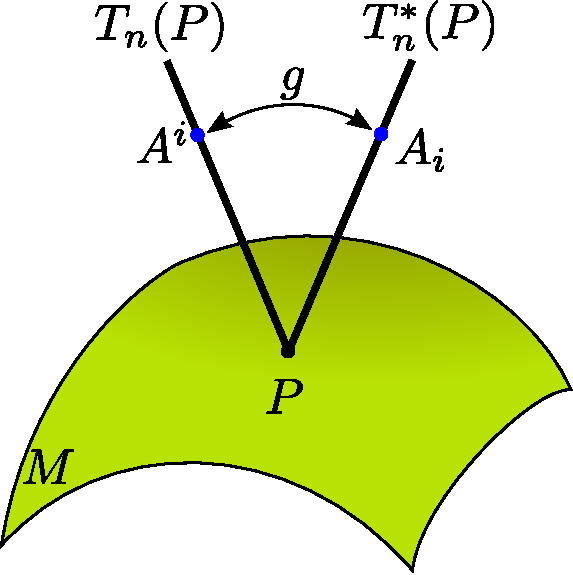
\includegraphics[height=6cm]{fig/fig-espacios-tangente-y-cotangente.pdf}}
\caption{El tensor m'etrico define una relaci'on uno a uno (isomorfismo) entre
los espacios tangente y cotangente en cada punto de la variedad.}
\label{5}
\end{figure}
\end{center}

El uso del tensor m'etrico para ``subir'' o ``bajar'' 'indices tambi'en es 'util para tensores de mayor rango. Por ejemplo, a partir del tensor de tipo $(^2_2)$, $T^{kl}{}_{i j}$, podemos definir el tensor de tipo $(^3_1)$:
\begin{equation}
T^{kl i}{}_j:=g^{im}T^{kl}{}_{mj},
\label{g10}
\end{equation}
etc.

\subsection{M'etrica inducida}
Considere una variedad $M$ de dimensi'on $n$ y una \textbf{subvariedad} $S$ de dimensi'on $d<n$. Entonces la m'etrica de $M$ \textit{induce la m'etrica sobre} $S$, ya que la distancia entre dos puntos arbitrarios de $S$ puede calcularse aplicando (o restringiendo) la distancia entre puntos infinitesimalmente pr'oximos de $M$ al caso particular de dos puntos infinitesimalmente pr'oximos de $S$. Si se usan coordenadas $x^i$ en (una vecindad de) $M$, y la subvariedad $S$ es definida por medio de una \textbf{parametrizaci'on} de la forma
\begin{equation}
x^i=x^i(y^a), \qquad a=1,\dots,d,
\end{equation}
donde $y^a$ son \textit{coordenadas sobre la subvariedad} $S$, entonces la diferencia de coordenadas de $M$ correspondiente a dos puntos infinitesimalmente pr'oximos de $S$ puede expresarse como
\begin{equation}
\left.dx^i\right|_{S}=\frac{\partial x^i}{\partial y^a}(x(y))\,dy^a.
\end{equation}
Con esto, podemos expresar el elemento de l'inea sobre $S$ como
\begin{align}
\left.dl^2\right|_{S}=&\left.g_{ij}(x)\right|_{S}\left.dx^i\right|_{S}\left.dx^j\right|_{S} \\
=& g_{ij}(x(y))\left(\frac{\partial x^i}{\partial y^a}dy^a\right)\left(\frac{\partial x^j}{\partial y^b}dy^b\right) \\
=& g_{ab}(y)dy^ady^b.
\end{align}
De esta forma, las componentes del tensor m'etrico inducido sobre $S$, en coordenadas $y^a$ est'a dadas por
\begin{equation}\marginnote{m'etrica inducida}\label{metind2}
\boxed{g_{ab}(y)= g_{ij}(x(y))\frac{\partial x^i}{\partial y^a}\frac{\partial x^j}{\partial y^b}.}
\end{equation}

Note que esta relaci'on \textit{no es} simplemente la usual ley de transformaci'on de las componentes del tensor m'etrico bajo una TGC, ya que $g_{ij}$ y $g_{ab}$ \textit{tienen dimensiones distintas} ($n$ y $d<n$ respectivamente) y son componentes de representan las \textit{m'etricas de dos variedades distintas} (pero relacionadas).

\subsection{Curvas geod'esicas}

Consideremos dos puntos $P$ y $Q$ en una variedad provista de m'etrica.
Se define la \textbf{geod'esica} como la curva \textit{de longitud m'inima  (extrema) entre} $P$ y $Q$.

Si $\cal C$ es una curva representada param'etricamente por
$x^i =x^i (\lambda)$, entonces $\cal C$ es una geod'esica entre $P$ y $Q$ si y
s'olo si\footnote{Suponemos, por simplicidad, pero sin perder generalidad, que el par'ametro $\lambda$ \textit{crece} desde $P$ a $Q$, de modo que en la integral $d\lambda>0$.}
\begin{equation}
L=\int_P^Qd\ell= \int_P^Q\sqrt{g_{ij}(x(\lambda))dx^idx^j}=\int_{\lambda i}^{\lambda_{f}}\sqrt{g_{ij}(x(\lambda))\frac{dx^i}{d\lambda}\frac{dx^j }{d\lambda}}\, d\lambda \label{gm1}
\end{equation}
es m'inima. Esto implica que su variaci'on respecto a peque\~nas desviaciones de la trayectoria geod'esica es nula:
\begin{equation}
\delta L=0. \label{gm2}
\end{equation}
La condici'on (\ref{gm2}) implica que las geod'esicas satisfacen las ecuaciones de Euler-Lagrange,
\begin{equation}
\frac{\delta L}{\delta x^i }=\frac{\partial \tilde{L}}{\partial x^i }-\frac
{d}{d\lambda}\left( \frac{\partial
\tilde{L}}{\partial\left(\frac{dx^i}{d\lambda}\right) }\right) =0,
\label{gm3}
\end{equation}
donde
\begin{equation}
\tilde{L}(x^i,\frac{dx^i}{d\lambda})=\sqrt{g_{ij}(x(\lambda))\frac{dx^i
}{d\lambda}\frac{dx^j }{d\lambda}}.
\label{gm4}
\end{equation}
De aqu'i, tenemos que
\begin{equation}
\frac{\partial\tilde{L}}{\partial x^k}=\frac{1}{2}(g_{lm}\dot{x}^l\dot{x}^m)^{-1/2}(\partial_k g_{ij})\dot{x}^i\dot{x}^j=\frac{1}{2\tilde{L}}(\partial_k g_{ij})\dot{x}^i\dot{x}^j,
\end{equation}
\begin{equation}
\frac{\partial\tilde{L}}{\partial \dot{x}^k}=\frac{1}{2}(g_{lm}\dot{x}^l\dot{x}^m)^{-1/2}(2g_{kj}\dot{x}^j)=\frac{1}{\tilde{L}}g_{kj}\dot{x}^j,
\end{equation}
\begin{equation}
\frac{d}{d\lambda}\left(\frac{\partial\tilde{L}}{\partial \dot{x}^k}\right)= -\frac{\dot{\tilde{L}}}{\tilde{L}^2}g_{kj}\dot{x}^j+\frac{1}{\tilde{L}}(\partial_l g_{kj})\dot{x}^j\dot{x}^l+\frac{1}{\tilde{L}}g_{kj}\ddot{x}^j.
\end{equation}
De esta forma, encontramos que
\begin{equation}
\frac{\delta L}{\delta x^i }=\frac{1}{2\tilde{L}}(\partial_k g_{ij})\dot{x}^i\dot{x}^j+\frac{\dot{\tilde{L}}}{\tilde{L}^2}g_{kj}\dot{x}^j-\frac{1}{\tilde{L}}(\partial_l g_{kj})\dot{x}^j\dot{x}^l-\frac{1}{\tilde{L}}g_{kj}\ddot{x}^j.
\end{equation}
Multiplicando por $\tilde{L}g^{ki}$ y reordenando t'erminos obtenemos
\begin{align}
\frac{\dot{\tilde{L}}}{\tilde{L}}\dot{x}^i &= \ddot{x}^i+g^{ik}(\partial_l g_{kj})\dot{x}^j\dot{x}^l-\frac{1}{2}(\partial_k g_{jl})\dot{x}^j\dot{x}^l \\
&= \ddot{x}^i+\frac{1}{2}g^{ik}\left(\partial_l g_{kj}+\partial_j g_{kl}-\partial_k g_{jl}\right)\dot{x}^j\dot{x}^l \\
&= \ddot{x}^i+\left\{ _{jl}^{\,i}\right\}\dot{x}^j\dot{x}^l.
\end{align}
Por lo tanto \eqref{gm3} es equivalente a 
\begin{equation}\marginnote{Ecuaci'on Geod'esicas}
\boxed{\frac{d^2x^i }{d\lambda^2}+\left\{ _{ j l}^{\, i}\right\}
\frac{dx^j }{d\lambda}\frac{dx^{ l}}{d\lambda}=f(\lambda)\frac{dx^{ i
}}{d\lambda},} \label{gm5}
\end{equation}
donde
\begin{equation}\marginnote{S'imbolos de Christoffel}
\boxed{\left\{ _{ jk}^{\,i}\right\}:=\frac{1}2g^{il}\left[
\partial_kg_{jl}+\partial_j g_{lk}-\partial_l g_{kj}\right] ,} \label{gm6}
\end{equation}
es llamado \textbf{s'imbolo de Christoffel}\footnote{En honor a Elwin Bruno Christoffel: 1829-1900, f'isico y matem'atico alem'an. Ver \url{http://es.wikipedia.org/wiki/Elwin_Bruno_Christoffel}.} (de segunda especie), y
\begin{equation}
f(\lambda):=\frac{\dot{\tilde{L}}}{\tilde{L}}=\frac{d\ }{d\lambda}\left(\ln\tilde{L}\right)=\frac{d\ }{d\lambda}\left(\ln\frac{d\ell}{d\lambda}\right) =\frac{\frac{d^2\ell}{d\lambda^2}}{\frac{d\ell}{d\lambda}}\label{efe}
\end{equation}
 es una funci'on que depende de la elecci'on del par'ametro $\lambda$ usado para parametrizar la curva. Note que aqu'i hemos impl'icitamente introducido una funci'on $\ell(\lambda)$, el largo de la curva desde el punto inicial $P_i$, dada por $\ell(\lambda):=\int_{\lambda_i}^\lambda \tilde{L}\,d\lambda$, de modo que $\tilde{L}=d\ell/ d\lambda$.

La relaci'on (\ref{efe}) determina la funci'on $f$ a partir de la relaci'on
entre la longitud propia de la curva y el par'ametro $\lambda$. De aqu'i es
directo verificar que un cambio de par'ametro $\lambda\to\lambda'$ implicar'a
un cambio en la funci'on $f$, de modo que
\begin{equation}\label{fpf}
f'=\left(\frac{d\lambda'}{d\lambda}\right)^{-1}\left[f-\frac{d\ }{d\lambda}\left(\ln\frac{d\lambda'}{d\lambda}\right)\right] .
\end{equation}
En efecto, como
\begin{equation}
\frac{d\ell}{d\lambda'}=\frac{d\ell}{d\lambda}\frac{d\lambda}{d\lambda'},
\end{equation}
\begin{equation}
\frac{d^2\ell}{d\lambda'^2}=\frac{d^2\ell}{d\lambda^2}\left(\frac{d\lambda}{d\lambda'}\right)^2+\frac{d\ell}{d\lambda}\frac{d^2\lambda}{d\lambda'^2},
\end{equation}
entonces
\begin{align}
f'&=\frac{\frac{d^2\ell}{d\lambda'^2}}{\frac{d\ell}{d\lambda'}} = \frac{\frac{d^2\ell}{d\lambda^2}\left(\frac{d\lambda}{d\lambda'}\right)^2+\frac{d\ell}{d\lambda}\frac{d^2\lambda}{d\lambda'^2}}{\frac{d\ell}{d\lambda}\frac{d\lambda}{d\lambda'}} =f\frac{d\lambda}{d\lambda'}+\frac{\frac{d^2\lambda}{d\lambda'^2}}{\frac{d\lambda}{d\lambda'}}
=f\frac{d\lambda}{d\lambda'}+\frac{d}{d\lambda'}\ln\left(\frac{d\lambda}{d\lambda'}\right),
\end{align}
que es equivalente a \eqref{fpf}.

Como consecuencia de la arbitrariedad de $\lambda$ es posible \textit{elegir par'ametros especiales que simplifiquen los c'alculos}. Por ejemplo, \textit{si $d\ell\neq 0$ sobre toda la geod'esica}, entonces podemos usar un \textbf{par'ametro af'in}, de la forma $\lambda_{\rm afin}:=\alpha\cdot \ell+\beta$, donde $\ell$ es la distancia \textit{sobre la curva} desde un punto de referencia hasta un punto arbitrario de ella, y adem'as $\alpha$ y $\beta$ son \textit{constantes} (escalares). En este caso (\ref{efe}) implica que $f=0$. Por simplicidad, usualmente se elige en estos casos la longitud (propia) de la curva ($\alpha=1$), de modo que la ecuaci'on de la geod'esica adopta la forma ``can'onica":
\begin{equation}\marginnote{Ec. Geod'esica c/param. af'in}
\boxed{\frac{d^2x^i }{d\ell^2}+\left\{ _{ j l}^{\, i}\right\}
\frac{dx^j }{d\ell}\frac{dx^{ l}}{d\ell}=0.} \label{gm7}%
\end{equation}

Por ejemplo, en el espacio euclidiano y en coordenadas cartesianas
$\left\{_{ j l}^{\, i}\right\}\overset{\ast}{=}0$, de modo que, de acuerdo con
(\ref{gm7}), las geod'esicas de este espacio son rectas con ecuaciones
$x^i (\ell)\overset{\ast}{=}x_0^i +\ell v_0^i $, con $x_0^i $ y $v_0^i$ constantes.

A partir de la ley de transformaci'on del tensor m'etrico puede verificarse f'acilmente que \textit{los s'imbolos de Christoffel no son componentes de un tensor bajo TGC's}, ya que
\begin{equation}
\overline{\left\{_{j k}^{\,\, i}\right\}}=\frac{\partial\bar{x}^i}{\partial x^l }\frac{\partial
x^p}{\partial\bar{x}^j }\frac{\partial x^q}{\partial\bar{x}^k }\,
\left\{_{p q}^{\,\, l}\right\} +\frac{\partial\bar{x}^i}{\partial x^l }\frac{\partial
^2x^l }{\partial\bar{x}^j \partial\bar{x}^k }. \label{dinv7}
\end{equation}

\subsection{Isometr'ias (simetr'ias de la m'etrica)}
\begin{center}
\begin{figure}[H]
\centerline{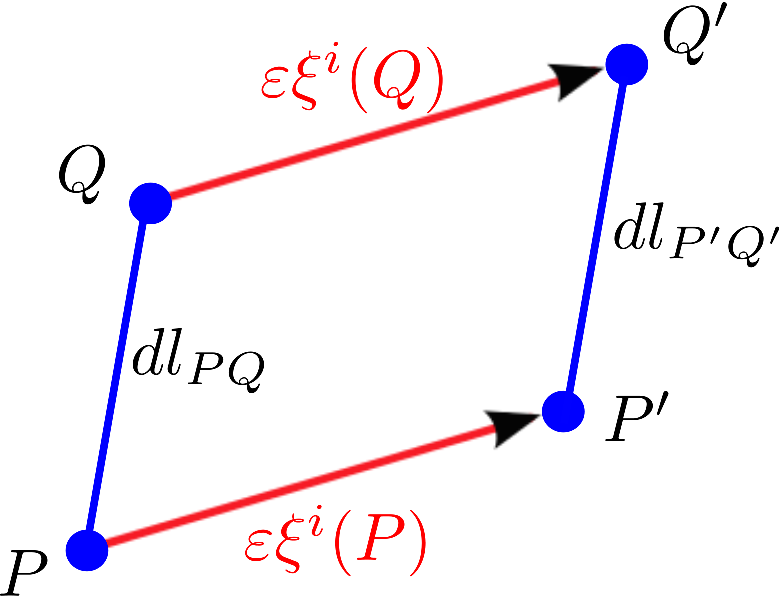
\includegraphics[height=5cm]{fig/fig-Killing.pdf}}
\caption{Trasladando puntos en la direcci'on $\xi^i(x)$.}
\label{fig:Killing}
\end{figure}
\end{center}
Las \textbf{isometr'ias} de una m'etrica (en caso de que existan) describen \textbf{direcciones de simetr'ia} de la m'etrica en (una regi'on de) la variedad, de una forma covariante, es decir, independiente del sistema de coordenadas usado. 

Sean $P$ y $Q$ dos puntos infinitesimalmente cercanos, con coordenadas $x^i$ y $x^i+dx^i$ respectivamente y $\xi^i=\xi^i(x)$ un campo vectorial (contravariante) definido en una vecindad que incluye a $P$ y $Q$. Como se muestra en la figura, podemos localizar dos nuevos puntos $P'$ y $Q'$ cuyas coordenadas est'an dadas por:%
\begin{align}
x^i(P')  & = x^i(P)+\varepsilon\,\xi^i(P)\label{is1},\\
x^i(Q')  & = x^i(Q)+\varepsilon\,\xi^i(Q), \label{is1b}
\end{align}
donde $\varepsilon$ es un par'ametro escalar infinitesimal. Los puntos $P'$ y $Q'$ son entonces los resultantes de ``trasladar'' los puntos $P$ y $Q$ en la direcci'on definida por el vector $\xi$. Se dice entonces que $\xi^i(x)$ describe una isometr'ia de la variedad, si para puntos arbitrarios $P$ y $Q$ se cumple que la distancia entre ellos es la misma que entre los puntos ``trasladados'' $P'$ y $Q'$, es decir, si
\begin{equation}
dl_{PQ}\stackrel{!}{=}dl_{P'Q'}  \label{is2}%
\end{equation}
o, m'as expl'icitamente,
\begin{align}
dl_{PQ}^2  &  =g_{ij}(P)(dx^i_{PQ})(dx^j_{PQ}) , \label{is3}\\
dl_{P'Q'}^2  &  =g_{ij}(P')(dx^i_{P'Q'})(dx^j_{P'Q'}) . \label{is4}
\end{align}
Usando (\ref{is1}), (\ref{is1b}) podemos escribir
\begin{align}
dx^i_{P'Q'} &= dx^i_{PQ}+\varepsilon\left[\xi^i(Q)-\xi^i(P)\right] \\
&= dx^i+\varepsilon\left[\xi^i(x+dx)-\xi^i(x)\right] \\
&= dx^i+\varepsilon \left[\partial_j\xi^i(x)\right]dx^j.
\end{align}
Con esta expresi'on (\ref{is4}) se reduce, a primer orden en $\varepsilon$, a
\begin{equation}
dl_{P'Q'}^2=g_{ij}dx^idx^j+\varepsilon\left[g_{ij}dx^idx^k\partial_k\xi^i
+g_{ij}dx^kdx^j\partial_k\xi^i+\xi^kdx^idx^j\partial_kg_{ij}\right],  \label{is5}
\end{equation}
donde ahora todos los campos est'an evaluados en el punto $P$, de coordenadas $x^i$.
Cambiando adecuadamente los 'indices de suma, la expresi'on (\ref{is5}) toma la forma
\begin{equation}
dl_{P'Q'}^2=g_{ij}dx^idx^j+\varepsilon\left[g_{ik}\partial_j\xi^k
+g_{kj}\partial_i\xi^k+\xi^k\partial_kg_{ij}\right] dx^idx^j,
\label{is6}%
\end{equation}
de modo que la condici'on (\ref{is2}) es equivalente a
\begin{equation}\marginnote{Ecuaci'on de Killing}
\boxed{g_{ik}\partial_j\xi^k+g_{kj}\partial_i\xi^k+\xi^k\partial_kg_{ij}=0.} \label{is8}
\end{equation}
ya que $\varepsilon$, $dx^i$ son infinitesimales, pero arbitrarios.

La ecuaci'on\footnote{M'as exactamente, las $n(n+1)/2$ ecuaciones.} diferencial parcial lineal (\ref{is8}) es la condici'on que debe satisfacer el campo $\xi^i$ para que describa una isometr'ia. Las soluciones (no nulas) son llamadas \textbf{vectores de Killing}\footnote{Wilhelm Karl Joseph Killing (1847-1923): matem'atico alem'an. Ver \url{http://en.wikipedia.org/wiki/Wilhelm_Killing}  \textbf{$\leftarrow$ se necesita traducci'on al espa\~nol de esto!}.}.

\subsubsection{Plano euclideano}

En el plano euclidiano y en coordenadas cartesianas, $x^i=(x,y)$, la
m'etrica es $g_{ij}\overset{\ast}{=}\delta_{ij}$.
%Luego, de la ecuaci'on (\ref{gm6}) tenemos que los s'imbolos de Christoffel son
%nulos. y por lo tanto la curvatura tambi'en es nula.
%
%La ecuaci'on de las geod'esicas (\ref{gm7}) es%
%\begin{equation}
%\frac{d^2x^i}{d\ell^2}=0. %
%\end{equation}
%Por lo tanto, las geod'esicas en el plano son rectas.
En este caso la ecuaci'on (\ref{is8}) se reduce a:
\begin{align}
\delta_{ik}\partial_j\xi^k+\delta_{kj}\partial_i\xi^k  &  =0,\label{isej1}\\
\partial_j\xi_i+\partial_i\xi_j  &  =0. \nonumber
\end{align}

Escribimos expl'icitamente estas ecuaciones:%
\begin{align}
\partial_1\xi^1+ & \partial_1\xi^1= 0, \label{isej2}\\
\partial_1\xi^2+ & \partial_2\xi^1= 0, \label{isej3} \\
\partial_2\xi^2+ & \partial_2\xi^2= 0.  \label{isej4}
\end{align}
De (\ref{isej2}) y de (\ref{isej4}) se obtiene respectivamente que $\xi
^1=\xi^1(y)$ y $\xi^2=\xi^2(x)$. De este modo la ecuaci'on (\ref{isej3}) toma la forma:
\begin{equation}
\frac{d\xi^2}{dx}+\frac{d\xi^1}{dy}=0.  \label{isej5}%
\end{equation}
Usando el hecho de que $x$ e $y$ son coordenadas independientes, vemos que
esta ecuaci'on se satisface si y s'olo si:
\begin{align}
\frac{d\xi^1}{dy}  &  =\alpha=\text{cte.},\label{isej6}\\
\frac{d\xi^2}{dx}  &  =-\alpha, \nonumber
\end{align}
de modo que:
\begin{equation}
\xi^1 =\alpha y+\beta, \qquad
\xi^2 =-\alpha x+\gamma. \label{isej7}
\end{equation}
Esta soluci'on se puede expresar como combinaci'on lineal de tres
soluciones linealmente independientes:
\begin{align}
\xi^i  &  =\left(  \xi^1,\xi^2\right)  \\
& =\left(  \alpha y+\beta,-\alpha x+\gamma\right) \\
  &  =\alpha\left(  y,-x\right)  +\beta\left(  1,0\right)
+\gamma\left(  0,1\right)  \\
 &  =\alpha\,\xi_{(1)}^i+\beta\,\xi_{(2)}^i+\gamma\,\xi_{(3)}^i, \nonumber
\end{align}
donde
\begin{align}
\xi_{(1)}^i  &  :=\left(  y,-x\right)  ,\\
\xi_{(2)}^i  &  :=\left(  1,0\right)  ,\\
\xi_{(3)}^i  &  :=\left(  0,1\right)  .
\end{align}
\begin{center}
\begin{figure}[H]
\centerline{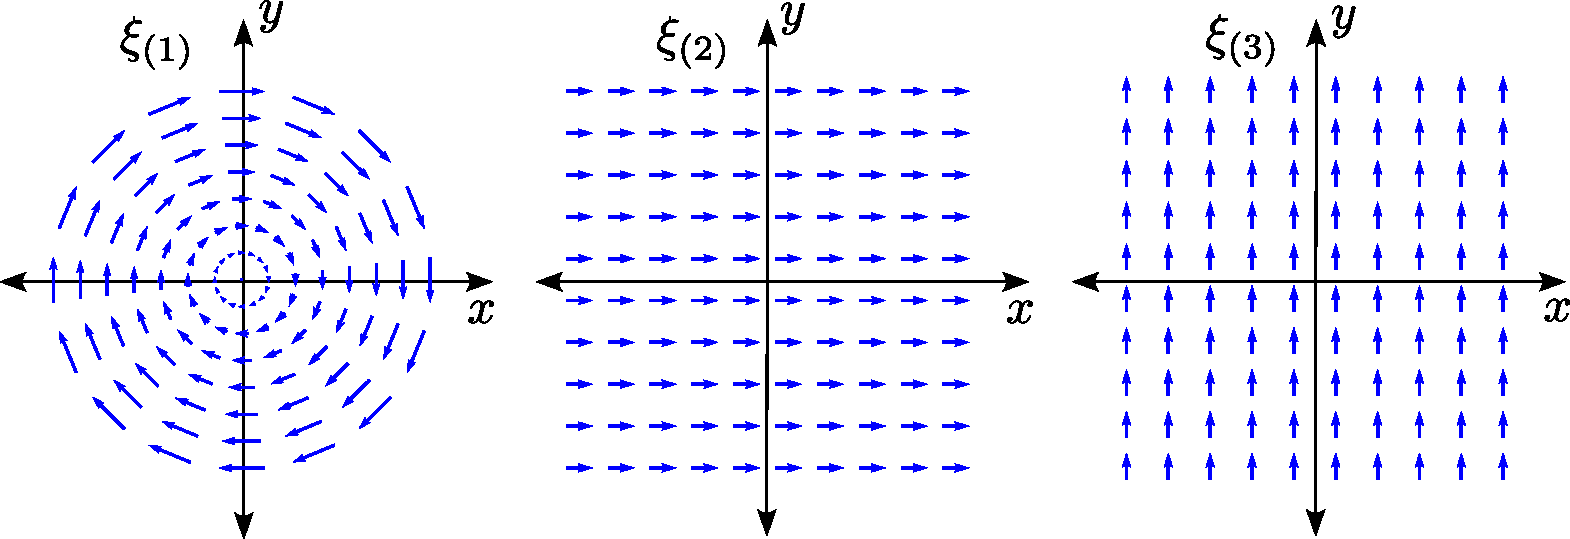
\includegraphics[height=4cm]{fig/fig-Killing-E2.pdf}}
\caption{Vectores de Killing en el plano euclideano bidimensional.}
\label{KE2}
\end{figure}
\end{center}
Los tres campos independientes $\xi^i_{(a)}$, $a=1,2,3$ son representados en la figura \ref{KE2}. Los vectores $\xi^i_{(1)}$ y $\xi^i_{(2)}$ corresponden a \textit{traslaciones} a lo largo de los ejes $x$ e $y$ respectivamente, mientras que $\xi^i_{(1)}$ a \textit{rotaciones} respecto al origen. Cualquier combinaci'on lineal (a coeficientes constantes) de estos tres vectores b'asicos define una direcci'on de simetr'ia del espacio Euclideano bidimensional.
\subsubsection{Esfera unitaria}

Consideremos como segundo ejemplo la m'etrica que el espacio euclidiano
tridimensional $E_{3}$ induce sobre la esfera unitaria. Sabemos que en
coordenadas cartesianas la m'etrica de $E_{3}$ es $g_{ij}=\delta_{ij}$ y la restricci'on a los puntos de la esfera es:
\begin{align}
x^1  &  =\sen\theta\cos\varphi,\\
x^2  &  =\sen\theta\sen\varphi,\\
x^{3}  &  =\cos\theta,
\end{align}
de modo que las coordenadas sobre la esfera son $\theta$ y $\varphi$. Usando
(\ref{metind2}) para calcular la m'etrica inducida, obtenemos
\begin{equation}
g_{ab}=\left(
\begin{array}[c]{cc}
1 & 0\\
0 & \sen^2\theta
\end{array}\right) ,  \label{ind7}
\end{equation}
donde $a,b=\theta,\varphi$. Usando (\ref{gm6}) obtenemos que las componentes no
nulas del s'imbolo de Christoffel son:
\begin{align}
\left\{  _{\varphi\varphi}^{\ \theta}\right\}  &  =-\sen\theta\cos\theta,\label{ind8}\\
\left\{  _{\theta\varphi}^{\, \varphi}\right\}   &  =\left\{  _{\varphi\theta}^{\,\varphi}\right\}  =\cot\theta.
\end{align}
%De este modo, se obtiene directamente que las ecuaciones para las
%geod'esicas sobre la esfera son:%
%\begin{align}
%\frac{d^2\theta}{d\ell^2}-\sen\theta\cos\theta\left(\frac{d\varphi}{d\ell}\right)^2  &  =0,\label{ind9}\\
%\frac{d^2\varphi}{d\ell^2}+2\cot\theta\frac{d\theta}{d\ell}\frac{d\varphi}{d\ell}  &  =0.
%\end{align}
%Tambi'en, mediante un c'alculo directo, encontramos que las componentes
%no nulas de la curvatura de la esfera son:%
%\begin{align}
%R_{\phi\theta\phi}^{\theta}  &  =-R_{\phi\phi\theta}^{\theta}=\sin^2%
%\theta,\label{ind10}\\
%R_{\theta\theta\phi}^{\phi}  &  =-R_{\theta\phi\theta}^{\phi}=-1. %
%\nonumber
%\end{align}

El sistema de ecuaciones para los vectores de Killing sobre la esfera unitaria,
seg\'{u}n (\ref{is8}) es:
\begin{align}
g_{\theta\theta}\partial_\theta\xi^\theta+g_{\theta\theta}\partial_\theta\xi^\theta +\xi^a\partial_ag_{\theta\theta}  &  =0,\label{isej12}\\
g_{\theta\theta}\partial_\varphi\xi^\theta+g_{\varphi\varphi}\partial_\theta\xi^\varphi +\xi^a\partial_ag_{\theta\varphi}  &  =0, \\
g_{\varphi\varphi}\partial_\varphi\xi^\varphi+g_{\varphi\varphi}\partial_\varphi\xi^\varphi +\xi^a\partial_ag_{\varphi\varphi}  &  =0.
\end{align}
Luego:
\begin{align}
\partial_\theta\xi^\theta  &  =0,\label{isej13}\\
\partial_\varphi\xi^\theta+\sen^2\theta\,\partial_\theta\xi^\varphi  &  =0, \\
2\sen^2\theta\,\partial_\varphi\xi^\varphi+\xi^\theta\partial_\theta(\sen^2\theta)  & =0.
\end{align}
La primera ecuaci'on nos dice que $\xi^\theta=\xi^\theta(\varphi)$, de modo que la
segunda y tercera ecuaci'on nos queda:
\begin{align}
\partial_\varphi\xi^\theta+\sen^2\theta\,\partial_\theta\xi^\varphi  &
=0,\label{isej14}\\
\sen\theta\,\partial_\varphi\xi^\varphi+\xi^\theta\cos\theta  &  =0.
\end{align}
Se puede verificar, reemplazando directamente en estas ecuaciones, que el
sistema tiene por soluci'on:
\begin{equation}
\xi^a=\alpha\,\xi^a_{(1)} +\beta\,\xi^a_{(2)} +\gamma\,\xi^a_{(3)}
,\label{isej15}
\end{equation}
con
\begin{eqnarray}
\xi^a_{(1)} &=&(\sen\varphi, \cot\theta\cos\varphi ), \\
\xi^a_{(2)} &=&(\cos\varphi,-\cot\theta\sen\varphi) , \\
\xi^a_{(3)} &=&(0,1).
\end{eqnarray}

\begin{center}
\begin{figure}[H]
\centerline{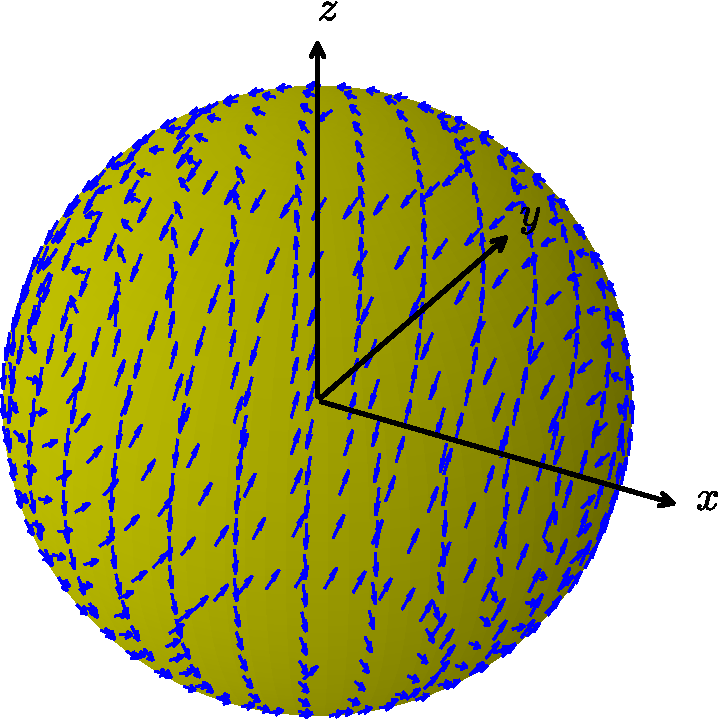
\includegraphics[height=4cm]{fig/fig-KS2x.pdf}\hfill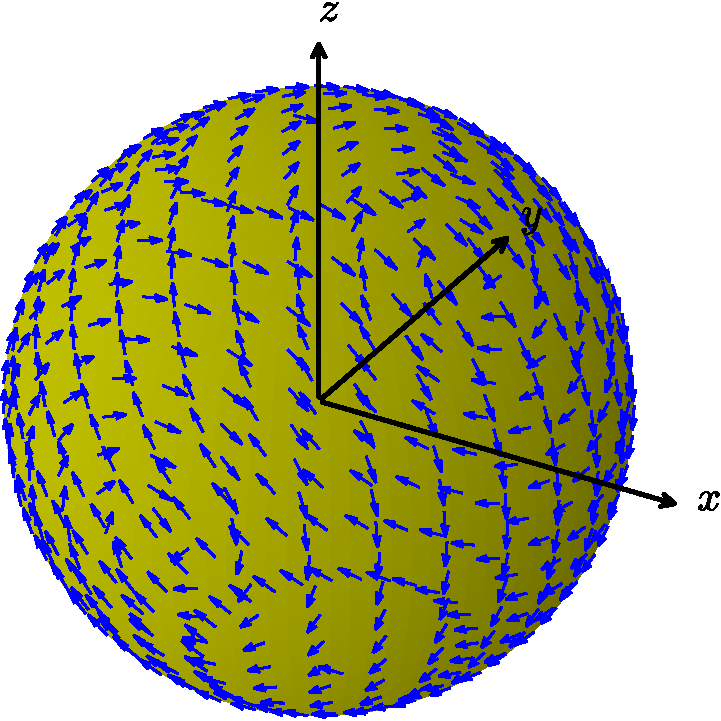
\includegraphics[height=4cm]{fig/fig-KS2y.pdf}\hfill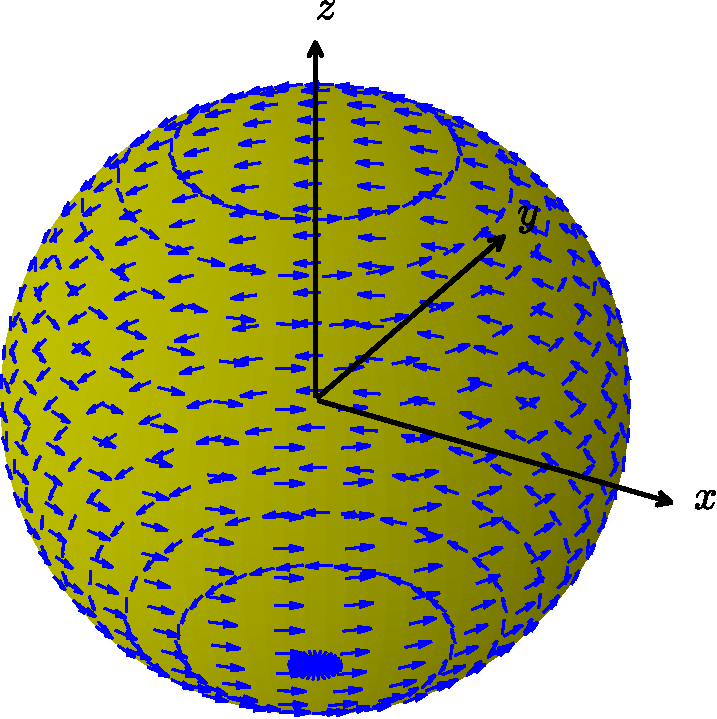
\includegraphics[height=4cm]{fig/fig-KS2z.pdf}}
\caption{Vectores de Killing sobre la esfera: 
$\xi^a_{(1)}$, $\xi^a_{(2)}$ y $\xi^a_{(3)}$ respectivamente.}
\label{KS2}
\end{figure}
\end{center}

\paragraph{Teorema:} El n'umero m'aximo de vectores de Killing independientes que una variedad de dimensi'on $n$ puede admitir es $n(n+1)/2$ *** Agregar ref. ***

***
\subsection{Coodenadas adaptadas a una isometr'ia}

Definimos una coordenada, por ejemplo, $x^1$, a lo largo de las l'ineas integrales del campo $\xi$, es decir, tal que los vectores tangentes a las l'ineas coordenadas de $x^1$ son paralelos a $\xi$. Esto implica que en el SC adaptado 
\begin{equation}
\xi^i\stackrel{*}{=}(\xi^1,0,\cdots,0).
\end{equation}
Siempre es posible definir la coordenada $x^1$ (en particular, qu'e tan r'apido var'ia 'esta sobre las curvas integrales de $\xi$) de modo que
\begin{equation}
\xi^i\stackrel{*}{=}(1,0,\cdots,0).
\end{equation}
Entonces, si $\xi$ es un vector de Killing, la ecuaci'on \eqref{is8} implica que
\begin{equation}
\partial_1g_{ij}\stackrel{*}{=}0,
\end{equation}
es decir, que en sistema de coordenadas adaptado al vector de Killing $\xi$ la m'etrica no depende de la coordenada adaptada $x^1$.

\subsection{Vectores de Killing y operadores diferenciales}
\begin{equation}
\hat{\xi}:=\xi^i\partial_i
\end{equation}

\section{Conexi'on, derivadas covariantes y transporte paralelo}

\subsection{Derivada parcial de campos tensoriales}

Salvo en el caso de un escalar, \textit{la derivada de las componentes de un tensor no define un nuevo tensor bajo TGC's}. Esto puede entenderse como una consecuencia del hecho que la definici'on de la derivada parcial de un tensor involucra (el l'imite) de la sustracci'on de tensores \textit{en puntos distintos}.

En efecto, veamos c'omo transforman las derivadas parciales $\partial_i
A_j:={\partial A_j}/{\partial x^i}$ de un vector covariante $A_i$:
\begin{equation}
\bar{\partial}_i\bar{A}_j=\frac{\partial \bar{A}_j}{\partial
\bar{x}^i}=\frac{\partial }{\partial \bar{x}^i}\left(\frac{\partial x^k
}{\partial\bar{x}^j }A_k \right)
=\frac{\partial x^k }{\partial\bar{x}^j }\frac{\partial x^l }{\partial\bar{x}^i}
\partial_l A_k +\frac{\partial^2 x^k }{\partial\bar
{x}^i \partial\bar{x}^j }A_k . \label{ord2}
\end{equation}
Vemos que la derivada parcial de un vector covariante se comporta como un tensor tipo $(_2^0)$ \textit{excepto por el segundo t'ermino}. La ley de
transformaci'on es lineal, pero inhomog'enea, lo que implica que si las
derivadas de un vector se anulan en un SC entonces 'estas no se anulan
necesariamente en otro.

Una consecuencia importante de este hecho es que, \textit{sin introducir elementos adicionales definidos sobre la variedad}, no existe un criterio \textit{independiente de coordenadas} de cu'ando un tensor es constante sobre (una regi'on de) la variedad. Esto se debe a que, como se deduce de la expresi'on \eqref{ord2}, aunque las componentes de un tensor sean iguales en dos puntos (o en una regi'on) de la variedad en alg'un SC ($x$, de modo que $\partial_iA_j=0$) en otros SC's ($\bar{x}$) 'este no ser'a el caso: $\bar{\partial}_i\bar{A}_j\neq 0$.
 
Lo mismo ocurre para tensores de distinto tipo. Por ejemplo, la ley de transformaci'on de un tensor tipo ($_2^0$) es:
\begin{equation}
\bar{A}_{jk}=\frac{\partial x^l}{\partial\bar{x}^j} \frac{\partial x^m}{\partial\bar{x}^k}A_{lm}. \label{ord3}
\end{equation}
Luego, sus derivadas parciales transforman bajo una TGC de la forma siguiente:
\begin{equation}
\bar{\partial}_i\bar{A}_{jk}=\frac{\partial x^l}{\partial\bar{x}^j} 
\frac{\partial x^m}{\partial\bar{x}^k} \frac{\partial x^n}{\partial \bar{x}^i}\,\partial_nA_{lm}+\left(
\frac{\partial^2 x^l}{\partial\bar{x}^i\partial\bar{x}^j} \frac{\partial x^m}{\partial\bar{x}^k} 
+\frac{\partial x^l}{\partial\bar{x}^j}\frac{\partial^2 x^m}{\partial\bar{x}^i\partial\bar{x}^k}\right) A_{lm}. \label{ord4}
\end{equation}

Vemos que los dos 'ultimos t'erminos en (\ref{ord4}) son lineales en las
componentes (no derivadas) del tensor original y son tambi'en lineales en las segundas derivadas del cambio de coordenadas. Estos t'erminos hacen que la ley de transformaci'on de las derivadas parciales difiera de la ley correspondiente a un tensor.

\subsubsection{Excepciones*}
Existen, sin embargo, ciertas combinaciones particulares de derivadas parciales que s'i son tensores. Por ejemplo, el ``rotor'' de un campo vectorial covariante $A_k $, $\partial_k A_i-\partial_iA_k $, es un tensor tipo ($_2^0$), ya que
\begin{align}
\bar{A}_k  & =\frac{\partial x^l}{\partial\bar{x}^k} A_l ,\label{ord6}\\
\bar{\partial}_i\bar{A}_k  & =\frac{\partial x^l}{\partial\bar{x}^k} 
\frac{\partial x^m}{\partial\bar{x}^i}\, \partial_mA_l +
\frac{\partial^2 x^l}{\partial\bar{x}^i\partial\bar{x}^k}\, A_l ,\\
\bar{\partial}_k \bar{A}_i & =\frac{\partial x^l}{\partial\bar{x}^i}
\frac{\partial x^m}{\partial\bar{x}^k}\, \partial_mA_l +
\frac{\partial^2 x^l}{\partial\bar{x}^k\partial\bar{x}^i}\, A_l ,\\
\end{align}
y por lo tanto
\begin{equation}
 \bar{\partial}_i\bar{A}_k -\bar{\partial}_k \bar{A}_i =\frac{\partial x^l}{\partial\bar{x}^k} \frac{\partial x^m}{\partial\bar{x}^i} \left( \partial_m A_l -\partial_l A_m\right) .
\end{equation}
De este modo, $\left(\partial_iA_j -\partial_j A_i\right)$ define un tensor
antisim'etrico de tipo ($_2^0$).

% \item La divergencia c'iclica de cualquier tensor antisim'etrico tipo
% ($_2^0$) es un tensor antisim'etrico tipo ($_{3}^0$). En efecto, sea
% $T_{ik}$ un tensor antisim'etrico. Entonces:
% \begin{equation}
% \bar{T}_{ik}=\frac{\partial x^l}{\partial\bar{x}^i} \frac{\partial x^m}{\partial\bar{x}^k} %
% T_{lm}. \label{ord8}%
% \end{equation}
% Queremos mostrar que \ $\partial_jT_{ik}+\partial_iT_{kj}+\partial
% _k T_{ji}$ es un tensor. Para esto calculemos dichos sumandos a partir de
% (\ref{ord8}):
% \begin{equation}
% \bar{\partial}_j\bar{T}_{ik}=\frac{\partial x^l}{\partial\bar{x}^i} \bar{\partial
% }_k x^m \bar{\partial}_jx^n\partial_nT_{lm}+\left(
% \bar{\partial}_j\frac{\partial x^l}{\partial\bar{x}^i} \,\frac{\partial x^m}{\partial\bar{x}^k} %
% +\frac{\partial x^l}{\partial\bar{x}^i} \,\bar{\partial}_j\frac{\partial x^m}{\partial\bar{x}^k} \right)
% T_{lm}, \label{ord9}%
% \end{equation}%
% \begin{equation}
% \bar{\partial}_i\bar{T}_{kj}=\frac{\partial x^l}{\partial\bar{x}^k} \bar{\partial
% }_jx^m \frac{\partial x^n}{\partial\bar{x}^i}\partial_nT_{lm}+\left(
% \bar{\partial}_i\frac{\partial x^l}{\partial\bar{x}^k} \,\bar{\partial}_jx^m %
% +\frac{\partial x^l}{\partial\bar{x}^k} \,\bar{\partial}_i\bar{\partial}_jx^m \right)
% T_{lm}, \label{ord10}%
% \end{equation}%
% \begin{equation}
% \bar{\partial}_k \bar{T}_{ji}=\frac{\partial x^l}{\partial\bar{x}^j} \bar{\partial
% }_ix^m \bar{\partial}_k x^n\partial_nT_{lm}+\left(
% \bar{\partial}_k \frac{\partial x^l}{\partial\bar{x}^j} \,\frac{\partial x^m}{\partial\bar{x}^i} %
% +\frac{\partial x^l}{\partial\bar{x}^j} \,\bar{\partial}_k \frac{\partial x^m}{\partial\bar{x}^i} \right)
% T_{lm}. \label{ord11}%
% \end{equation}
% Si se suman los tres t'erminos, se combinan adecuadamente los 'indices
% mudos $l$, $m$ y $n$, y se usan las propiedades de antisimetr'ia de $T$,
% se obtiene:
% \begin{equation}
% \bar{\partial}_j\bar{T}_{ik}+\bar{\partial}_i\bar{T}_{kj}+\bar{\partial
% }_k \bar{T}_{ji}=\frac{\partial x^l}{\partial\bar{x}^i} \frac{\partial x^m}{\partial\bar{x}^k} \text{
% }\bar{\partial}_jx^n\left( \partial_nT_{lm}+\partial_l T_{mn}%
% +\partial_mT_{nl}\right), \label{ord12}%
% \end{equation}
% lo cual prueba que la divergencia c'iclica de un tensor antisim'etrico
% tipo ($_2^0$) es un tensor antisim'etrico tipo ($_{3}^0$).


Todo esto no es suficiente para establecer un an'alisis tensorial
exhaustivo sobre una variedad. Una (aparentemente simple) pregunta a'un no tiene respuesta: \textquestiondown Qu'e condici'on caracteriza un campo vectorial
\textit{constante}? Claramente la respuesta \underline{no es}
$\partial_iA_j=0$, pues esta condici'on no es independiente del SC usado. De hecho, sin estructuras adicionales definidas sobre la variedad, el concepto de ``campo vectorial constante"\, simplemente no est'a definido. La estructura adicional que permite formular 'este y otros conceptos, por ejemplo el de derivada covariante, es llamada \textbf{conexi'on}.

\subsection{Conexi'on y derivada covariante de tensores}

\textbf{Definici'on:} Llamamos \textbf{conexi'on}\footnote{Tambi'en llamada \textbf{conexi'on af'in} o \textbf{afinidad}.}, $\Gamma$, \textit{a un arreglo de} $n^3$ \textit{cantidades definidas en cada punto de la variedad para las cuales:}
\begin{itemize}
\item Suponemos un conjunto de valores dados en cada SC particular y,
\item Cambian sus valores bajo una TGC de acuerdo a la siguiente ley de transformaci'on:
\begin{equation}\marginnote{Conexi'on}
\bar{\Gamma}_{\ jk}^i=\frac{\partial\bar{x}^i}{\partial x^l }\frac{\partial
x^p}{\partial\bar{x}^j }\frac{\partial x^q}{\partial\bar{x}^k }\,
\Gamma_{\ pq}^l +\frac{\partial\bar{x}^i}{\partial x^l }\frac{\partial
^2x^l }{\partial\bar{x}^j \partial\bar{x}^k }. \label{dinv72}
\end{equation}
\end{itemize}
A partir de una conexi'on y de un campo vectorial (covariante) es posible definir la siguiente combinaci'on, que es un tensor bajo TGC's:
\begin{equation}
\boxed{\nabla_iA_j:=\partial_iA_j-\Gamma_{\ ji}^kA_k.}
\label{dinv6}
\end{equation}
El tensor $\nabla_iA_j$ es llamado la \textbf{derivada covariante} de $A_j$ \textit{con respecto a la conexi'on} $\Gamma$. Se debe notar que $\Gamma$ est'a definida \textit{sobre} nuestra variedad y puede ser concebida,\textit{ en general}, como un objeto geom'etrico \textit{no necesariamente relacionado con una  m'etrica}.


Es simple verificar a partir de \eqref{ord2} y \eqref{dinv6} que $\nabla_iA_j$ es efectivamente covariante (es decir, un tensor), si suponemos que las componentes de $\Gamma$ transforman de acuerdo a \eqref{dinv72}.

Note que el segundo t'ermino del lado derecho de \eqref{dinv72} es independiente de $\Gamma$ y depende entonces s'olo de la transformaci'on de coordenadas. Esta es la propiedad implica que una conexi'on $\Gamma$ no sea nula en todo SC, a'un cuando puede serlo en algunos. Otra consecuencia de la ley de transformaci'on \eqref{dinv72} es que si \textit{dos conexiones}, $\Gamma$ y $\hat{\Gamma}$, definidas en la misma variedad, entonces \textit{su diferencia es un tensor}. En efecto, bajo una TGC se tiene que
\begin{align}
\bar\Gamma_{\ ik}^n-\hat{\overline{\Gamma}}{}^n_{\ ik} & =\frac{\partial
\bar{x}^n}{\partial x^l }\frac{\partial x^r}{\partial\bar{x}^i }
\frac{\partial x^s}{\partial\bar{x}^k }\,\Gamma_{\ rs}^l +\frac{\partial
\bar{x}^n}{\partial x^l }\frac{\partial^2 x^l }{\partial\bar{x}^i \partial\bar{x}^k }-\frac{\partial\bar{x}^n}{\partial x^l }
\frac{\partial x^r}{\partial\bar{x}^i }\frac{\partial x^s}{\partial
\bar{x}^k }\,\hat{\Gamma}_{\ rs}^l -\frac{\partial\bar{x}^n}{\partial x^l}\frac{\partial^2 x^l }{\partial\bar{x}^i \partial\bar{x}^k}\label{dinv8}\\
& =\frac{\partial
\bar{x}^n}{\partial x^l }\frac{\partial x^r}{\partial\bar{x}^i }
\frac{\partial x^s}{\partial\bar{x}^k }\left( \Gamma_{\ rs}^l
-\hat{\Gamma}_{\ rs}^l \right) .\nonumber
\end{align}
Luego, la diferencia $\Gamma_{jk}^i -\hat{\Gamma}_{jk}^i $ es un tensor. Equivalentemente, la suma de una conexi'on y un tensor de tipo $(_2^1)$ es una nueva conexi'on.

% Veamos qu'e sucede si sumamos dos afinidades, $\Gamma_{lm}^k $ y
% $\hat{\Gamma}_{lm}^k $:
% \begin{align}
% \bar\Gamma_{\ ik}^n+\overline{\hat{\Gamma}}_{ik}^n & =\frac{\partial
% \bar{x}^n}{\partial x^l }\frac{\partial x^r}{\partial\bar{x}^i }%
% \frac{\partial x^s}{\partial\bar{x}^k }\Gamma_{\ rs}^l +\frac{\partial
% \bar{x}^n}{\partial x^l }\frac{\partial^2 x^l }{\partial\bar{x}%
% ^i \partial\bar{x}^k }+\frac{\partial\bar{x}^n}{\partial x^l }%
% \frac{\partial x^r}{\partial\bar{x}^i }\frac{\partial x^s}{\partial
% \bar{x}^k }\hat{\Gamma}_{rs}^l +\frac{\partial\bar{x}^n}{\partial x^l %
% }\frac{\partial^2 x^l }{\partial\bar{x}^i \partial\bar{x}^k %
% },\label{dinv9}\\
% \bar\Gamma_{\ ik}^n+\overline{\hat{\Gamma}}_{ik}^n & =\frac{\partial
% \bar{x}^n}{\partial x^l }\frac{\partial x^r}{\partial\bar{x}^i }%
% \frac{\partial x^s}{\partial\bar{x}^k }\left( \Gamma_{\ rs}^l +\hat{\Gamma
% }_{rs}^l \right) +2\frac{\partial\bar{x}^n}{\partial x^l }\frac
% {\partial^2 x^l }{\partial\bar{x}^i \partial\bar{x}^k }.\nonumber
% \end{align}
%
%
% Luego la suma de dos afinidades no es una afinidad. Pero si $\lambda$ y $\mu$
% son n'umeros tales que $\lambda+\mu=1$ entonces tenemos:
% \begin{align}
% \lambda\bar\Gamma_{\ ik}^n+\mu\overline{\hat{\Gamma}}_{ik}^n &
% =\lambda\frac{\partial\bar{x}^n}{\partial x^l }\frac{\partial x^r%
% }{\partial\bar{x}^i }\frac{\partial x^s}{\partial\bar{x}^k }\Gamma
% _{rs}^l +\lambda\frac{\partial\bar{x}^n}{\partial x^l }\frac{\partial
% ^2x^l }{\partial\bar{x}^i \partial\bar{x}^k }+\mu\frac{\partial\bar
% {x}^n}{\partial x^l }\frac{\partial x^r}{\partial\bar{x}^i }%
% \frac{\partial x^s}{\partial\bar{x}^k }\hat{\Gamma}_{rs}^l +\mu
% \frac{\partial\bar{x}^n}{\partial x^l }\frac{\partial^2 x^l }%
% {\partial\bar{x}^i \partial\bar{x}^k }\label{dinv10}\\
% \lambda\bar\Gamma_{\ ik}^n+\mu\overline{\hat{\Gamma}}_{ik}^n &
% =\frac{\partial\bar{x}^n}{\partial x^l }\frac{\partial x^r}{\partial
% \bar{x}^i }\frac{\partial x^s}{\partial\bar{x}^k }\left( \lambda
% \Gamma_{\ rs}^l +\mu\hat{\Gamma}_{rs}^l \right) +\lambda\frac{\partial\bar
% {x}^n}{\partial x^l }\frac{\partial^2 x^l }{\partial\bar{x}^i %
% \partial\bar{x}^k }+\mu\frac{\partial\bar{x}^n}{\partial x^l }%
% \frac{\partial^2 x^l }{\partial\bar{x}^i \partial\bar{x}^k }\nonumber\\
% \lambda\bar\Gamma_{\ ik}^n+\mu\overline{\hat{\Gamma}}_{ik}^n &
% =\frac{\partial\bar{x}^n}{\partial x^l }\frac{\partial x^r}{\partial
% \bar{x}^i }\frac{\partial x^s}{\partial\bar{x}^k }\left( \lambda
% \Gamma_{\ rs}^l +\mu\hat{\Gamma}_{rs}^l \right) +\frac{\partial\bar{x}^n%
% }{\partial x^l }\frac{\partial^2 x^l }{\partial\bar{x}^i \partial\bar
% {x}^k }.\nonumber
% \end{align}
%
%
% Por lo tanto, $\lambda\Gamma_{\ rs}^l +\mu\hat{\Gamma}_{rs}^l $ es una
% afinidad si y s'olo si $\lambda+\mu=1$.

 La noci'on de derivada covariante introducida en (\ref{dinv6}) no es un concepto intr'inseco, ``natural'' de una variedad, sino que est'a definida a partir de una conexi'on, la cual debe ser indicada. Adem'as, es posible introducir m'as que una conexi'on sobre la misma variedad, por lo que es en general necesario distinguir entre las derivadas definidas con respecto a distintas conexiones.

Se extender'a ahora la noci'on de derivada covariante a tensores de distinto tipo. Existen distintas formas de motivar la definici'on de derivadas covariantes de tensores de tipo arbitrario. Una manera simple es  \textit{asumiendo} que la derivaci'on covariante satisface:
\begin{itemize}
\item[i)] la usual regla de la derivaci'on de un producto (regla de
Leibniz\footnote{En honor de Gottfried Leibniz: 1646-1716, fil'osofo, matem'atico, jurista, bibliotecario y pol'itico alem'an. Ver \url{http://es.wikipedia.org/wiki/Gottfried_Leibniz}.}) cuando se aplica al producto de tensores y,
\item[ii)] que la derivada covariante de un escalar coincide con la usual derivaci'on parcial.
\end{itemize}

A partir de estas propiedades es posible deducir la forma de la derivada covariante de cualquier cantidad tensorial. Por ejemplo, la derivada $\nabla_iB^j$ de un vector contravariante $B^j$ puede encontrarse aplicando las propiedades arriba descritas al escalar $A_k B^k $, donde $A_k$ son las componentes de un vector covariante (auxiliar). En efecto, la propiedad ii) implica que
\begin{equation}
\nabla_i\left( A_k B^k\right)=\partial_i\left( A_k B^k \right).\label{dinv12}
\end{equation}
Usando ahora la propiedad i), es decir, la regla de Leibniz podemos escribir
\begin{equation}
A_k (\nabla_iB^k)+(\nabla_i A_k)B^k = A_k (\partial_iB^k) +(\partial_iA_k)B^k .
\end{equation}
Finalmente, usando \eqref{dinv6} encontramos que
\begin{equation}
A_k (\nabla_iB^k) +\left(\partial_iA_k-\Gamma_{\ ki}^jA_j\right) B^k=A_k (\partial_iB^k) +(\partial_iA_k)B^k 
\end{equation}
Cancelando t'erminos y renombrando 'indices apropiadamente, podemos
escribir:
\begin{equation}
A_k \left( \nabla_iB^k -\partial_iB^k -\Gamma_{\ ji}^k B^j\right) =0,
\end{equation}
pero $A_k $ es arbitrario, de modo que el t'ermino entre par'entesis debe anularse para cada valor del 'indice $k$. De aqu'i podemos despejar una expresi'on expl'icita para la derivada covariante de un vector contravariante:
\begin{equation}
\boxed{\nabla_iB^k =\partial_iB^k +\Gamma_{\ ji}^kB^j .} \label{dinv15}
\end{equation}

Para un tensor general $T^{kl\cdots }{}_{pq\cdots }$ aplicamos un m'etodo similar. Consideramos la derivada covariante del escalar
\begin{equation}
T^{kl\cdots }{}_{pq\cdots }A_k B_l \cdots F^pG^q, \label{dinv16}
\end{equation}
donde $A_k $, $B_l $, $\dots $, $F^p$ y $G^q$ vectores arbitrarios. Se obtiene
as'i que la derivada covariante del tensor $T^{kl\cdots }{}_{pq\cdots}$ consta de su derivada parcial y de t'erminos adicionales, uno por
cada 'indice de $T^{kl\cdots }{}_{pq\cdots }$, cada uno de los cuales consta de
una contraci'on entre las componentes de $T^{kl\cdots }{}_{pq\cdots }$ y
$\Gamma$:
\begin{align}\marginnote{Derivada Covariante de un Tensor}
\nabla_iT^{kl\cdots }{}_{pq\cdots} =&\ \partial_iT^{kl\cdots
}{}_{pq\cdots}+\Gamma_{\ ni}^kT^{nl\cdots}{}_{pq\cdots } +\Gamma_{\
ni}^lT^{kn\cdots }{}_{pq\cdots} +\cdots \nonumber \\
&  -\Gamma_{pi}^nT^{kl\cdots}{}_{nq\cdots
}-\Gamma_{qi}^nT^{kl\cdots }{}_{pn\cdots }-\cdots . \label{dinv17}
\end{align}

Note que, \textit{de acuerdo a nuestras convenciones}, el 'indice de diferenciaci'on es siempre el segundo 'indice covariante de $\Gamma$ y los restantes lugares son llenados de modo de asignar el que falta de $T^{kl\cdots }{}_{pq\cdots }$.

Con el concepto de derivada covariante es posible definir el concepto de un
campo tensorial \textbf{covariantemente constante}: un campo tensorial es
(covariantemente) constante si y s'olo si su derivada covariante es nula.


\subsection{Transporte paralelo*}

Una forma interesante de entender los conceptos de derivada covariante y de
conexi'on es introduciendo la noci'on de \textbf{transporte paralelo}. Hemos visto que la derivada parcial de un campo vectorial covariante no define un tensor, ya que, por definici'on 'esta resta vectores definidos en distintos puntos (a'un cuando sean infitesimalmente pr'oximos):
\begin{equation}
\partial_jA_i(x):=\lim_{\Delta x^j \rightarrow0}\frac{A_i(x +\Delta x)-A_i(x)}{\Delta x^j }. \label{tp1}
\end{equation}
An'alogamente, podemos escribir:
\begin{eqnarray}
\nabla_jA_i&=&\partial_jA_i-\Gamma_{\ ij}^kA_k \\
&=& \lim_{\Delta x^j\rightarrow0}\frac{A_i(x+\Delta x)-A_i(x)}{\Delta x^j }-\Gamma_{\ ij}^kA_k \\
&=& \lim_{\Delta x^j\rightarrow0}\frac{A_i(x+\Delta x)-A_i(x)-\Gamma_{\
il}^k(x)A_k(x)\Delta x^l}{\Delta x^j }\\
&=& \lim_{\Delta x^j\rightarrow0}\frac{A_i(x+\Delta x)-\left[A_i(x)+\Gamma_{\
il}^k(x)A_k(x)\Delta x^l\right]}{\Delta x^j }\\
&=& \lim_{\Delta x^j\rightarrow0}\frac{A_i(x+\Delta x)-A^T_i(x+\Delta x)}{\Delta x^j }.
\end{eqnarray}
Basados en esto, definimos (en el punto con coordenadas $x+dx$) el vector $A^T_i(x+dx)$ por:
\begin{equation}\marginnote{transporte vector covariante}
 \boxed{A^T_i(x+dx):=A_i(x)+\Gamma_{\ il}^k(x)A_k(x)dx^l=A_i(x)+\delta A_i(x),} \label{tranAcov}
\end{equation}
que interpretaremos geom'etricamente como el vector resultante de \textit{transportar}
(``\textit{paralelamente}'') el vector $A_i(x)$ desde el punto con coordenadas $x$ hasta el punto con coordenadas $x+dx$. De esta forma, la derivada covariante de $A_i$ puede
ser interpretada como el l'imite de la diferencia de dos vectores definidos en el \textit{mismo punto}: el vector $A_i(x+dx)$ y el vector $A^T_i(x+dx)$ resultante de transportar $A_i(x)$ desde $x$ hasta $x+dx$.

An'alogamente, la derivada covariante de un vector contravariante $A^i$ puede
ser interpretada como el l'imite de la diferencia del vector $A^i(x+dx)$ y el
vector $A_T^i(x+dx)$ resultante de transportar $A^i(x)$ desde $x$ hasta $x+dx$,
con
\begin{equation}\marginnote{transporte vector contravariante}
 \boxed{A_T^i(x+dx):=A^i(x)-\Gamma_{\ jk}^i(x)A^j(x)dx^k=A^i(x)+\delta
A^i(x).}\label{tranAcontr}
\end{equation}

El proceso anterior puede repetirse de forma an'aloga para definir
el transporte paralelo de un tensor de rango arbitrario. Para esto, es 'util notar que 
\eqref{tranAcov} y \eqref{tranAcontr} pueden ser escritas como
\begin{equation}
A^T_i(x+dx):=A_i(x)+dx^j\left[\partial_jA_i-\nabla_jA_i\right],
\end{equation}
\begin{equation}
A_T^i(x+dx):=A^i(x)+dx^j\left[\partial_jA^i-\nabla_jA^i\right].
\end{equation}
Similarmente, para un tensor $A^{i_1\cdots i_r}_{\ \ \ \ \ \ j_1\cdots j_s}$ de tipo $(^r_s)$ tendremos que
\begin{equation}
(A_T)^{i_1\cdots i_r}_{\ \ \ \ \ \ j_1\cdots j_s}(x+dx):=A^{i_1\cdots i_r}_{\ \ \ \ \ \ j_1\cdots j_s}(x)+dx^j\left[\partial_j-\nabla_j\right]A^{i_1\cdots i_r}_{\ \ \ \ \ \ j_1\cdots j_s}.
\end{equation}


\subsection{Integrabilidad*}\label{sec:integ}
Habiendo definido el transporte paralelo de un vector (o, en
general, de un tensor) desde un punto $P$
de coordenadas $x^i $ a un punto $Q$ de coordenadas $x^i +dx^i$, podemos
ahora realizar una \textbf{sucesi'on de transportes} para definir el transporte de un vector \textit{a lo largo de una curva dada}. La pregunta natural que surge es si el transporte de un vector sobre una curva depende de la trayectoria usada o, por el contrario depende s'olo de los puntos iniciales y finales. Equivalentemente, podemos preguntarnos si al transportar un vector por una curva \textit{cerrada}, volviendo as'i al punto $P$ de partida, se obtiene o no el vector original.
\begin{center}
\begin{figure}[H]
\centerline{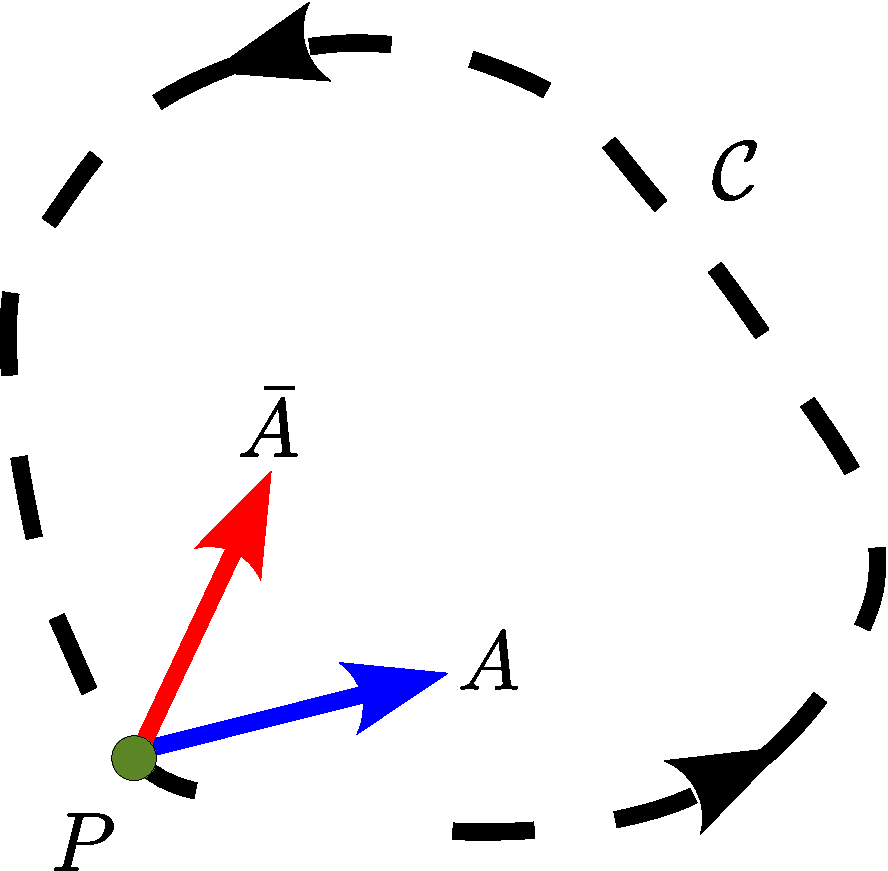
\includegraphics[height=5cm]{fig/fig-transporte-curva-cerrada.pdf}}
\caption{Transporte paralelo de un vector sobre una curva cerrada.}
\label{dibujo}
\end{figure}
\end{center}
\begin{quotation}
\textbf{Definici'on:} Decimos que una conexi'on $\Gamma$ es \textit{integrable} si y s'olo si el transporte asociado a ella es independiente de la trayectoria.
\end{quotation}
Encontremos las condiciones que debe satisfacer una conexi'on para que sea
integrable.
Para ello, consideremos un vector contravariante $A^i(P)$ asociado a un punto
$P$ de coordenadas $x^i$. Si el transporte es independiente de la trayectoria
usada, entonces puede definirse en forma 'unica un campo vectorial $A^i(x)$ (en todo punto de la variedad) transportando el vector $A^i(P)$ desde $P$ hasta cada punto de la variedad. En este caso podemos expresar el vector en un punto $Q$ infinitesimalmente
pr'oximo a $P$ como
\begin{equation}
A^i(x+dx)=A^i_T(x+dx) . \label{condint}
\end{equation}
Usando $A^i(x+dx)=A^i(x)+(\partial_j A^i)dx^j $ y (\ref{tranAcontr}) obtenemos que
la condici'on (\ref{condint}) es equivalente a
\begin{equation}
\nabla_j A^k=\partial_j A^k+\Gamma_{\ ij}^k A^i =0.
\label{ecdeintegr}%
\end{equation}
\begin{quotation}
\textbf{Resumiendo: si una conexi'on es integrable, existen vectores (no nulos) covariantemente constantes.}
\end{quotation}
Por otro lado, puede considerarse a (\ref{ecdeintegr}) como una ecuaci'on
diferencial que determina el campo (covariantemente constante) $A^i(x)$ dada la conexi'on, suponiendo que 'esta es integrable. Las \textbf{condiciones de
integrabilidad} de esta ecuaci'on son por lo tanto las condiciones para que la
conexi'on sea integrable.


\subsection{No-conmutatividad de las derivadas covariantes, curvatura y torsi'on}\label{sec:RT}
Las segundas derivadas covariantes de un tensor \textit{no conmutan}.
Por ejemplo, usando (\ref{dinv15}) y (\ref{dinv17}) podemos calcular la segunda derivada covariante de un vector arbitrario $A^i$:
\begin{equation}
\nabla_i \nabla_jA^k =\partial_i \partial_jA^{k
}+\partial_i A^l\Gamma_{\ lj}^k +A^l\partial
_i \Gamma_{\ lj}^k +\partial_jA^l\Gamma_{\ li}^k
+A^l\Gamma_{\ lj}^{m}\Gamma_{\ mi}^k -\partial_{l}A^k \Gamma_{\
ji}^l-A^l\Gamma_{\ lm}^k \Gamma_{\ ji}^{m}. \label{segder1}
\end{equation}
A partir de aqu'i, encontramos la siguiente identidad\footnote{Existen identidades similares para cada tipo de tensor. Por ejemplo: $\left[\nabla_i \nabla_j -\nabla_j\nabla_i\right]\phi\equiv T_{\ ij}^{k} \nabla_k\phi$,  $\left[\nabla_i \nabla_j -\nabla_j\nabla_i\right]A_k\equiv -R_{\ kij}^lA_l+T_{\ ij}^{l} \nabla_lA_k$. Es un buen ejercicio demostrar estas identidades ...}
\begin{equation}
\boxed{\nabla_i \nabla_jA^k -\nabla_j\nabla_i A^{k}\equiv R_{\ lij}^k
A^l+T_{\ ij}^{m} \nabla_mA^k ,} \label{cdc}
\end{equation}
donde hemos definido el \textbf{tensor de curvatura} como:
\begin{equation}\marginnote{Curvatura}
\boxed{R_{\ lij}^k :=\partial_i\Gamma_{\ lj}^k -\partial_j\Gamma_{\ li}^k 
+\Gamma_{\ mi}^k \Gamma_{\ lj}^m -\Gamma_{\ mj}^k \Gamma_{\ li}^m .}
\label{curvatura}
\end{equation}
Adem'as, definimos el \textbf{tensor de torsi'on} como:
\begin{equation}\marginnote{Torsi'on}
\boxed{T_{\ ij}^k :=\Gamma_{\ ij}^k -\Gamma_{\ ji}^k .}
\end{equation}

Aunque la curvatura y la torsi'on se definen en t'erminos de la conexi'on,
que no es un tensor, $R_{\ lij}^k$ y $T_{\ ij}^k$ s'i son tensores, como
puede verificarse considerando la consistencia de \eqref{cdc}, o directamente
a partir de su definici'on y la ley de transformaci'on \eqref{dinv72} de la conexi'on.

Note que, como consecuencia directa de su definici'on, estos tensores poseen las siguientes propiedades de antisimetr'ia:
\begin{equation}
R_{\ lij}^k\equiv - R_{\ lji}^k, \qquad T_{\ ij}^k\equiv -T_{\ ji}^k. \label{asRT}
\end{equation}
Estas simetr'ias, reducen el n'umero de componentes linealmente independientes de la curvatura y la torsi'on de \textit{una conexi'on arbitraria} a $n^3(n-1)/2$ y $n^2(n-1)/2$, respectivamente.

Retornando a la identidad \eqref{cdc}, vemos que ella implica que la derivada covariante es independiente del orden de derivaci'on (cuando se aplica a un vector arbitrario) si y s'olo si $R_{\ lji}^k=0$ y $T_{\ ij}^{k}=0$.

Por otro lado, si existe un sistema coordenado donde $\Gamma_{\ ij}^k
\overset{\ast}{=}0$ \textit{en todo punto de una regi'on dada}, entonces la curvatura y la torsi'on ser'an id'enticamente nulas, $R_{\ ijk}^l =0$ y $T_{\ ij}^{k}=0$, en esa regi'on. Adem'as, como la curvatura y la torsi'on son tensores, 'estas se anular'an en todo sistema coordenado.
El contrarec'iproco tambi'en es v'alido. Si existe un sistema
coordenado en el cual la curvatura o la torsi'on sean distintas de cero, $R_{\ ijk}^l \neq 0$ 'o $T_{\ ij}^{k}\neq 0$, entonces no existir'a ning'un sistema coordenado en el cual la conexi'on se anule en la regi'on dada.

Tambi'en es posible probar (aunque es bastante m'as laborioso, y omitiremos la prueba aqu'i. Ver, por ejemplo, la secci'on 6.7 de \cite{Dinverno}) que si la curvatura y la torsi'on de anulan en una regi'on de la variedad entonces es posible encontrar un SC tal que la conexi'on se anule en ese sistema.

En resumen:
\begin{quotation}
\textbf{La condici'on necesaria y suficiente para encontrar un sistema coordenado donde todas las componentes de la conexi'on se anulen en todo punto de una regi'on dada, $\Gamma_{\ ij}^k \overset{\ast}{=}0$, es que $R_{\ ijk}^l=0$ y $T_{\ ij}^k =0$ en esa regi'on.}
\end{quotation}

\subsection{Interpretaci'on geom'etrica de la curvatura*}
\begin{center}
\begin{figure}[h!]
\centerline{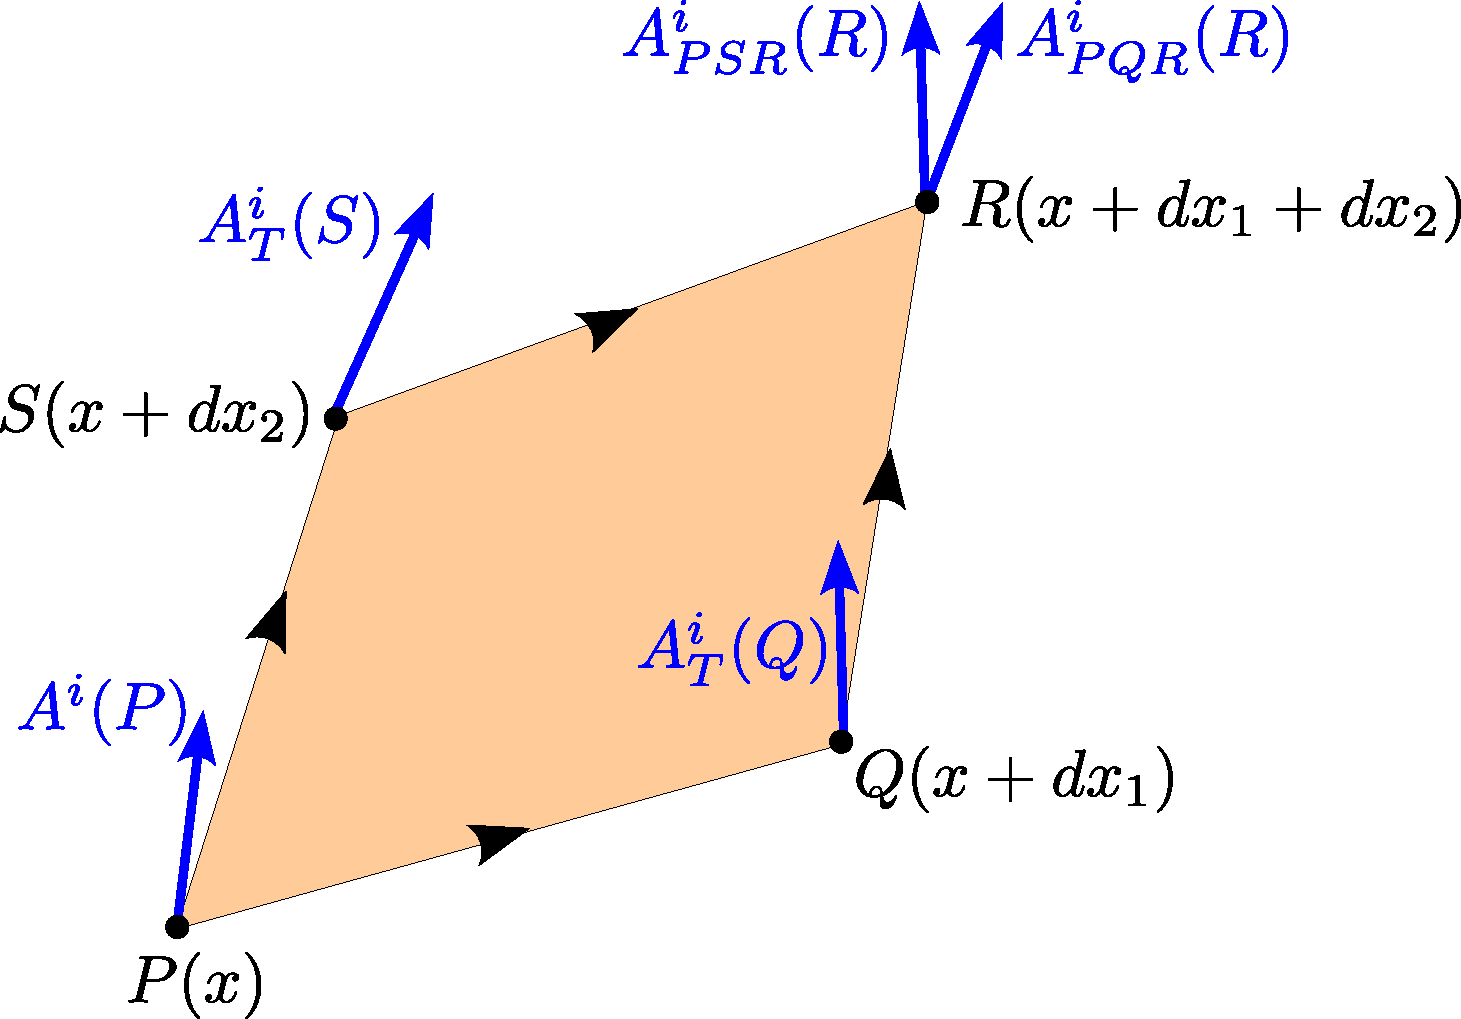
\includegraphics[height=6cm]{fig/fig-transporte-y-curvatura-01.pdf}}
\caption{Transporte de un vector desde $P$ a $R$ por dos trayectorias (infinitesimales) distintas.}
\label{intgeomcurv}
\end{figure}
\end{center}

Consideremos cuatro puntos $P,Q,R$ y $S$ como en la figura (\ref{intgeomcurv}), con coordenadas $x^i $, $x^i+dx_1^i$, $x^i+dx_1^i+dx_2^i$ y $x^i+dx_2^i$ respectivamente.
Sean $A^i (P)$ las componentes de un vector contravariante definido en el punto $P$. Traslademos este vector a trav'es de la trayectoria $PQR$, obteniendo $\bar{A}^i_{PQR}(R)$, y compar'emoslo con el vector resultante del transporte por la trayectoria $PSR$, $\bar{A}^i_{PSR}(R)$.

Transportamos primero $A^i$ de $P$ a $Q$, obteniendo el vector $A_{T}^i(Q)$:
\begin{equation}
A_{T}^i(Q)=A^i(P) -\Gamma_{\ jk}^i(P)A^j(P)\, dx_1^k .
\label{AT1}%
\end{equation}

Transportamos ahora $A_{T}^i $ desde $Q$ hasta $R$, obteniendo as'i el vector denotado por $A_{PQR}^i (R)$:
\begin{equation}
A_{PQR}^i (R) = A_{T}^i (Q) -\Gamma_{\ jk}^i(Q)A_{T}^j (Q)\,dx_2^k. \label{AT2}%
\end{equation}
 La conexi'on en el lado derecho de (\ref{AT2}) est'a evaluada en el punto $Q$, de coordenadas $x^i +dx_1^i$, y por lo tanto podemos escribir
\begin{equation}
\Gamma_{\ jk}^i(Q)=\Gamma_{\ jk}^i (x+dx_1)=\Gamma_{\ jk}^i(x)+dx_1^l(\partial_l\Gamma_{\ jk}^i) (x) . \label{expGam}
\end{equation}
Reemplazando \eqref{expGam} en \eqref{AT2} y utilizando (\ref{AT1}) obtenemos:%
\begin{align}
A_{PQR}^i (R) &= A^i -\Gamma_{\ jk}^i A^j\,dx_1^k-\Gamma_{\ jk}^i A^j\,dx_2^k \nonumber\\
& \quad  +\Gamma_{\ jk}^i \Gamma_{\ lm}^jA^l\, dx_1^m\,dx_2^k -(\partial_l\Gamma_{\ jk}^i) A^j dx_1^l dx_2^k. \label{AT22}
\end{align}
El c'alculo del vector $A_{\rm PSR}^i(R)$ es an'alogo, con la 'unica diferencia que primero se realiza el desplazamiento coordenado $dx_2^i$ hasta el punto $S$ y luego el desplazamiento en $dx_1^i$ hasta el punto $R$. Por lo tanto, el vector buscado tiene la misma forma que \eqref{AT22}, pero intercambiando $dx_1^i$ con $dx_2^i$, es decir,
\begin{align}
A_{PSR}^i (R) &= A^i -\Gamma_{\ jk}^i A^j\,dx_2^k-\Gamma_{\ jk}^i A^j\,dx_1^k \nonumber\\
& \quad  +\Gamma_{\ jk}^i \Gamma_{\ lm}^jA^l\, dx_2^m\,dx_1^k -(\partial_l\Gamma_{\ jk}^i) A^j dx_2^l dx_1^k. \label{APSR}
\end{align}

%Desplazamos ahora $A_{T2}^i $ desde $R$ hasta $S$, obteniendo $A_{T3}^i (S)$:
%\begin{equation}
%A_{T3}^i (S) = A_{T2}^i(R) -\Gamma_{\ jk}^i(R)A_{T2}^j (R)(-dx_1^k). \label{AT3}%
%\end{equation}
%Aqu'i hemos tomado en cuenta que la diferencia de coordenadas entre los puntos involucrados es $x^i(S)-x^i(R)=-dx_1^k$. Adem'as,
%\begin{equation}
%\Gamma_{\ jk}^i(R)=\Gamma_{\ jk}^i (x+dx_1+dx_2)=\Gamma_{\ jk}^i(x)+(dx_1^l+dx_2^l)(\partial_l\Gamma_{\ jk}^i) (x) . \label{expGam2}
%\end{equation}
%Reemplazando (\ref{expGam2}) en (\ref{AT3}) y utilizando (\ref{AT2}) obtenemos:%
%\begin{equation}
%A_{T3}^i (S) = A^i-\Gamma_{\ jk}^i A^j\,dx_2^k +\left(\partial_k\Gamma_{\ jl}^i-\partial_l\Gamma_{\ jk}^i+\Gamma_{\ mk}^i \Gamma_{\ jl}^m-\Gamma_{\ ml}^i \Gamma_{\ jk}^m\right) A^j\,dx_2^k\,dx_1^l. \label{AT32}
%\end{equation}
%
% Finalmente, trasladamos el vector $A_{T3}^i (S)$ hasta el punto inicial $P$:
%\begin{equation}
%A_{T4}^i(P) = A_{T3}^i(S) -\Gamma_{\ jk}^i(S)A_{T3}^j (S)(-dx_2^k). \label{AT4}%
%\end{equation}
%Usamos $\Gamma_{\ jk}^i(S)=\Gamma_{\ jk}^i(x+dx_2)=\Gamma_{\ jk}^i(x)+dx_2^l(\partial_l\Gamma_{\ jk}^i) (x)$ y nuestro resultado anterior (\ref{AT32}) y finalmente encontramos
%\begin{equation}
%A_{T4}^i(P) =A^i+\left(\partial_k\Gamma_{\ jl}^i-\partial_l\Gamma_{\ jk}^i+\Gamma_{\ mk}^i \Gamma_{\ jl}^m-\Gamma_{\ ml}^i \Gamma_{\ jk}^m\right) A^j\,dx_2^k\,dx_1^l.
%\end{equation}
%Vemos que el segundo t'ermino del lado derecho es precisamente el tensor de curvatura (\ref{curvatura}). As'i obtenemos:
%\begin{equation}
%\boxed{(A_{T4}^i -A^i)(x) =R_{\ jkl}^i(x)\, A^j(x)\,dx_2^k\,dx_1^l.} \label{19}%
%\end{equation}

Comparamos ambos vectores transportado calculando la diferencia de sus componentes. Restando \eqref{AT22} y \eqref{APSR} obtenemos (luego de renombrar algunos 'indices) que el resultado es proporcional al tensor de curvatura \eqref{curvatura},
\begin{equation}
\boxed{(A_{PSR}^i-A^i_{PQR})(R) =R_{\ jkl}^i(x)\, A^j(x)\,dx_1^k\,dx_2^l.} \label{19}%
\end{equation}
%Por lo tanto, la diferencia entre el vector transportado y el original es
%proporcional a la curvatura.
Esto demuestra que el tensor de curvatura de una conexi'on mide localmente (en una regi'on infinitesimal) la magnitud de la dependencia del transporte (inducido por la conexi'on, de vectores y tensores) con la trayectoria.

La relaci'on \eqref{19} que implica que, si la curvatura es nula, el transporte de cualquier vector es independiente de la trayectoria en una regi'on infinitesimal. Este resultado puede extenderse a trayectorias finitas que unan extremos comunes considerando una sucesi'on de ``deformaciones infinitesimales'' de una curva en otra, tal como lo ilustra la figura. Para esto, suponemos que la variedad ``no tiene agujeros'', es decir, que es \textbf{simplemente conexa}. Por lo tanto, si el tensor de curvatura es nulo y la variedad es simplemente conexa entonces el transporte es independiente de la trayectoria, es decir, la conexi'on es integrable.

\subsection{Interpretaci'on geom'etrica de la torsi\'on*}
Consideremos tres puntos $P$, $Q$ y $S$ de la variedad, infinitesimalmente
cercanos, tal que las coordenadas de $P$ son $x^i $, $dx_1^i $ es la
diferencia de las coordenadas entre los puntos $P$ y $Q$, y $dx_2^k $ es la
diferencia de las coordenadas entre los puntos $P$ y $S$ (ver figura \ref{fig:torsion}a). 
Ahora transportamos los vectores contravariantes $dx_1^k $ y $dx_2^k $, ambos definidos en $P$, hasta los puntos $S$ y $Q$, para obtenener as'i $\overline{dx}^i_1$ y $\overline{dx}^i_2$, respectivamente (ver figura \ref{fig:torsion}b). Las componentes de estos nuevos vectores (infinitesimales) est'an dadas entonces por
\begin{center}
\begin{figure}[H]
\centerline{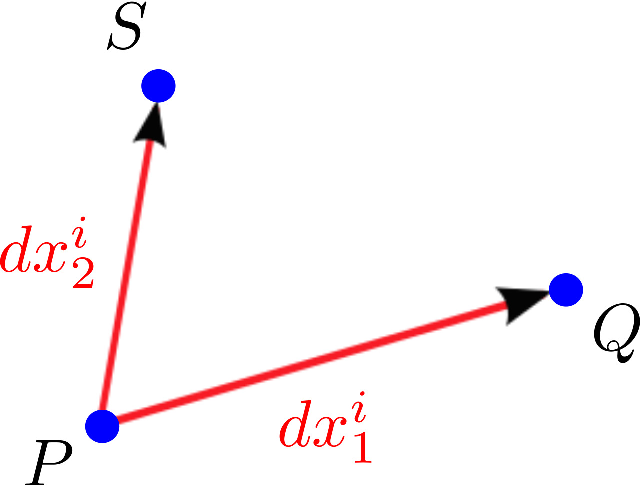
\includegraphics[height=4cm]{fig/fig-torsion-01.pdf}
\hspace{1cm}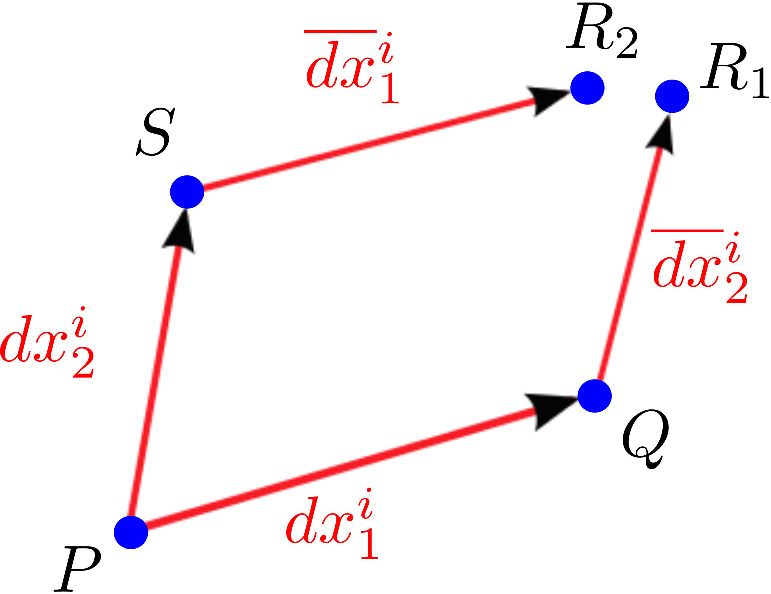
\includegraphics[height=4cm]{fig/fig-torsion-02.pdf}}
\caption{}
\label{fig:torsion}
\end{figure}
\end{center}
\begin{equation}
\overline{dx}_2^i (Q)=dx_2^i -\Gamma_{\ jk}^i(x)\, dx_2^j dx_1^k ,
\end{equation}
\begin{equation}
\overline{dx}_1^i (S)=dx_2^i -\Gamma_{\ jk}^i(x)\, dx_1^j dx_2^k .
\end{equation}

Los nuevos vectores $\overline{dx}_2^i (Q)$ y $\overline{dx}_1^i (S)$ permiten definir nuevos puntos $R_1$ y $R_2$, cuyas coordenadas son
\begin{equation}
x^i(R_1):=x^i(Q)+\overline{dx}_2^i (Q)=x^i+dx_1^i+dx_2^i -\Gamma_{\ jk}^i(x)\, dx_2^j dx_1^k, 
\end{equation}
\begin{equation}
x^i(R_2):=x^i(S)+\overline{dx}_1^i (S)=x^i +dx_2^i +dx_1^i
 -\Gamma_{\ jk}^i(x)\, dx_1^j dx_2^k .
\end{equation}
En general, los puntos $R_1$ y $R_2$ \textit{no coinciden}: la diferencia entre sus coordenadas est'a dada por
\begin{align}
x^i(R_2)-x^i(R_1) &= -\Gamma_{\ jk}^i(x)\, dx_1^j dx_2^k+ \Gamma_{\ jk}^i(x)\, dx_2^j dx_1^k \\
&=  \left[-\Gamma_{\ jk}^i(x)+ \Gamma_{\ kj}^i(x)\right] dx_1^j dx_2^k \\
&=  -T_{\ jk}^i(x)\, dx_1^j dx_2^k .
\end{align}
Vemos entonces que en la construcci'on geom'etrica discutida de un ``paralel'ogramo infinitesiamal'' los puntos finales no coinciden (el ``paralel'ogramo no se cierra'') si el tensor de torsi'on en no nulo. Debido a esto a menudo se dice que la torsi'on describe (posibles) ``fallas en el cierre local de paralel'ogramos infinitesimales''.



%\subsection{Integrabilidad y curvatura*}
%Vimos en la secci'on \ref{sec:integ} que si una conexi'on es integrable entonces
%existen campos vectoriales no nulos $A^i(x)$ tal que $\nabla_iA^j=0$. Usando esto y la identidad (\ref{cdc}) encontramos el siguiente resultado:
%\begin{quotation}
%\textbf{Teorema:} Si una conexi'on es integrable entonces su tensor de curvatura es nulo.
%\end{quotation}
%Equivalentemente, si el tensor de curvatura de una conexi'on es no nulo, 'esta no es integrable.
%
%Puede tambi'en ser probado que el rec'iproco del teorema anterior es t'ambi'en v'alido. Para esto, usamos \eqref{19} que implica que, si la curvatura es nula, el transporte de cualquier vector es independiente de la trayectoria en una regi'on infinitesimal. Este resultado puede extenderse a trayectorias finitas generales considerando una sucesi'on de ``deformaciones infinitesimales'' de una curva en otra, tal como lo ilustra la figura. Para esto, asumimos que la variedad ``no tiene agujeros'', es decir, que es \textbf{simplemente conexa}.
%
%En resumen:
%\begin{quotation}
%\textbf{Teorema:} Una conexi'on es integrable si y s'olo si su curvatura es
%igual a cero.
%\end{quotation}
% Estas condiciones de integrabilidad pueden obtenerse de la forma usual: las
% segundas derivadas parciales $A^i $ deben conmutar, es decir,
% \begin{equation}
% \frac{\square A^k }{\partial x^m \partial x^j }=\frac{\square %
% A^k }{\partial x^j \partial x^m }. \label{segder}%
% \end{equation}
% De las ecuaciones (\ref{ecdeintegr}) y (\ref{segder}) se obtiene la
% condici'on:
% \begin{equation}
% \frac{\partial}{\partial x^m }\left( \Gamma_{\ ij}^k A^i \right)
% -\frac{\partial}{\partial x^j }\left( \Gamma_{im}^k A^i \right) =0.
% \label{exac}%
% \end{equation}
% Desarrollando obtenemos que%
% \begin{equation}
% A^i \partial_m\Gamma_{\ ij}^k +\Gamma_{\ ij}^k \partial_mA^i %
% -A^i \partial_j\Gamma_{im}^k -\Gamma_{im}^k \partial_jA^i =0.
% \label{10}%
% \end{equation}
% Reemplazando $\partial_jA^k $ en (\ref{10}) tenemos:%
% \begin{align}
% A^i \partial_m\Gamma_{\ ij}^k -A^i \partial_j\Gamma_{im}^k +\Gamma
% _{lm}^k \Gamma_{\ ij}^l A^i -\Gamma_{lj}^k \Gamma_{im}^l A^i  & =0,\\
% A^i \left( \partial_m\Gamma_{\ ij}^k -\partial_j\Gamma_{im}^k %
% +\Gamma_{lm}^k \Gamma_{\ ij}^l -\Gamma_{lj}^k \Gamma_{im}^l \right)  & =0.
% \label{12}%
% \end{align}
% Como $A^i $ es un vector arbitrario, la condici'on de integrabilidad es:%
% \begin{equation}
% \partial_m\Gamma_{\ ij}^k -\partial_j\Gamma_{im}^k +\Gamma_{lm}^k %
% \Gamma_{\ ij}^l -\Gamma_{lj}^k \Gamma_{im}^l =0.
% \end{equation}


Por ejemplo, en el caso de un plano ($E_2$) sabemos que el transporte es independiente de la trayectoria, y por lo tanto la conexi'on es integrable. Adem'as, en coordenadas cartesianas\footnote{Utilizamos el s'imbolo $\overset{\ast}{=}$ para denotar que esta igualdad es v'alida s'olo en un sistema coordenado particular.} $\Gamma_{\ ij}^k \overset{\ast}{=}0$. En este caso,
seg'un (\ref{curvatura}), tenemos que la curvatura se anula, $R_{\ ijk}^l =0$.

%\subsection{Condiciones de Integrabilidad}\label{sec-ci}
%Puesto que el an'alisis realizado es s'olo fruto de reescribir la
%ecuaci'on del movimiento de una part{\'\i}cula libre en un SR
%no-inercial, debe entonces ser posible, dados $\bar{\Gamma }$ y/o
%$\bar{g}$ en alg'un SR, retornar a un SRI con sus coordenas inerciales asociadas. En
%este caso (compare (\ref{tsri}) y (\ref{tsrni})) la conexi'on $\Gamma$ se anula
%id'enticamente y la m'etrica adopta su forma minkowskiana. En otras palabras, un SRI queda determinado por los requerimientos que $g_{\mu\nu }=\eta _{\mu\nu }$ y $%
%\Gamma _{\ \mu\nu }^\lambda =0$ \emph{globalmente}, es decir, en todo punto del
%espaciotiempo.
%
%Estudiaremos ahora las condiciones que las componentes de una conexi'on
%$\bar{\Gamma }$ en un sistema coordenado $\bar x$ deben satisfacer de modo que
%exista la transformaci'on $\bar{x}\to x$ de vuelta a un SRI.
%
%De la ley de transformaci'on (\ref{tigam}) vemos que la condici'on para que en
%el nuevo sistema de coordenadas $\Gamma=0$ es
%\begin{equation}
%\frac{\partial x^\mu}{\partial \bar{x}^\sigma }\frac{\partial \bar{x}^\rho
%}{\partial x^{\nu }}\frac{\partial\bar{x}^{\eta }}{\partial
%x^\lambda}\bar{\Gamma }_{\ \rho \eta}^\sigma (\bar{x})+\frac{\partial x^{\mu
%}}{\partial \bar{x}^\rho }\frac{\partial ^2\bar{x}^\rho }{\partial
%x^{\nu}\partial x^\lambda }=0.
%\end{equation}
%De aqu'i, obtenemos
%\begin{equation}
%\frac{\partial ^2\bar{x}^\alpha }{\partial x^{\nu }\partial
%x^\lambda }=-\frac{\partial \bar{x}^\rho }{\partial x^{\nu }}%
%\frac{\partial \bar{x}^{\eta }}{\partial x^\lambda }\bar{%
%\Gamma }_{\ \rho \eta }^\alpha (\bar{x}) .\label{2der}
%\end{equation}
%
%Ya que, asumiendo que la transformaci'on $\bar{x}\to x$ existe, el lado
%izquierdo de (\ref{2der}) es sim'etrico bajo intercambio de los 'indices $\nu$
%y $\lambda$, debe cumplirse que el lado derecho tambi'en lo sea. Esta
%condici'on es equivalente a
%\begin{equation}
%\boxed{\bar{\Gamma }_{\ \mu\nu}^\lambda
%=\bar{\Gamma}_{\ \nu\mu}^\lambda.}
%\end{equation}
%
%Otra condici'on puede ser encontrada usando el hecho que el lado derecho de
%(\ref{2der}) debe efectivamente ser igual a las segundas derivadas de las
%funciones que definen el cambio de coordenadas. Para esto, derivamos
%(\ref{2der}) nuevamente y obtenemos:
%\begin{eqnarray}
%\frac{\partial ^3\bar{x}^\alpha }{\partial x^\rho \partial
%x^{\nu }\partial x^\lambda } &=&-\frac{\partial }{\partial x^\rho }\left(
%\frac{\partial \bar{x}^\beta }{\partial x^{\nu }}\frac{\partial
%\bar{x}^{\gamma }}{\partial x^\lambda }\bar{\Gamma }_{\ \beta
%\gamma }^\alpha \right) \\
%\frac{\partial ^3\bar{x}^\alpha }{\partial x^\rho \partial
%x^{\nu }\partial x^\lambda } &=&-\left[ \frac{\partial ^2\bar{x}%
%^\beta }{\partial x^\rho \partial x^{\nu }}\frac{\partial \bar{x}%
%^{\gamma }}{\partial x^\lambda }\bar{\Gamma }_{\ \beta \gamma
%}^\alpha +\frac{\partial \bar{x}^\beta }{\partial x^{\nu }}%
%\frac{\partial ^2\bar{x}^{\gamma }}{\partial x^\lambda \partial
%x^\rho }\bar{\Gamma }_{\ \beta \gamma }^\alpha +\frac{\partial
%\bar{x}^\beta }{\partial x^{\nu }}\frac{\partial \bar{x}%
%^{\gamma }}{\partial x^\lambda }\frac{\partial \bar{x}^{\delta }}{%
%\partial x^\rho }\frac{\partial \bar{\Gamma }_{\ \beta \gamma
%}^\alpha }{\partial \bar{x}^{\delta}}\right].
%\end{eqnarray}%
%Reemplazando, las segundas derivadas usando (\ref{2der}) nuevamente, llegamos
%a
%\begin{eqnarray}
%\frac{\partial ^3\bar{x}^\alpha }{\partial x^\rho \partial
%x^{\nu }\partial x^\lambda }&=&\frac{\partial \bar{x}^\sigma }{%
%\partial x^\rho }\frac{\partial \bar{x}^{\eta }}{\partial x^{\nu }}%
%\bar{\Gamma }_{\ \sigma \eta }^\beta \frac{\partial \bar{x}%
%^{\gamma }}{\partial x^\lambda }\bar{\Gamma }_{\ \beta \gamma
%}^\alpha +\frac{\partial \bar{x}^\beta }{\partial x^{\nu }}%
%\frac{\partial \bar{x}^\sigma }{\partial x^\lambda }\frac{\partial
%\bar{x}^{\eta }}{\partial x^\rho }\bar{\Gamma }_{\ \sigma \eta
%}^{\gamma }\bar{\Gamma }_{\ \beta \gamma }^\alpha -\frac{\partial
%\bar{x}^\beta }{\partial x^{\nu }}\frac{\partial \bar{x}%
%^{\gamma }}{\partial x^\lambda }\frac{\partial \bar{x}^{\delta }}{%
%\partial x^\rho }\frac{\partial \bar{\Gamma }_{\ \beta \gamma
%}^\alpha }{\partial \bar{x}^{\delta }} \\
%&=&-\frac{\partial \bar{x}^\beta }{\partial x^{\nu }}\frac{%
%\partial \bar{x}^{\gamma }}{\partial x^\lambda }\frac{\partial
%\bar{x}^{\delta }}{\partial x^\rho }\left( \frac{\partial \bar{%
%\Gamma }_{\ \beta \gamma }^\alpha }{\partial \bar{x}^{\delta }}
%-\bar{\Gamma }_{\sigma\gamma }^\alpha \bar{\Gamma }_{\ \delta \beta
%}^\sigma -\bar{\Gamma }_{\ \beta \sigma }^\alpha \bar{\Gamma }_{\ \gamma
%\delta }^\sigma \right).
%\end{eqnarray}
%Nuevamente, ya que el lado izquierdo de esta expresi'on debe ser sim'etrico
%bajo intercambio de los 'indices $\lambda$ y $\rho$, es decir,
%\begin{equation}
%\frac{\partial ^3\bar{x}^\alpha }{\partial x^\rho \partial
%x^{\nu }\partial x^\lambda }\equiv\frac{\partial ^3\bar{x}^\alpha }{\partial
%x^\lambda \partial x^{\nu }\partial x^\rho },
%\end{equation}
%obtenemos la siguiente condici'on para las componentes de $\bar\Gamma$ y sus
%derivadas:
%\begin{equation}
%\frac{\partial \bar{\Gamma }_{\ \beta \gamma }^{\alpha
%}}{\partial \bar{x}^{\delta }}-\bar{\Gamma }_{\ \sigma \gamma
%}^\alpha \bar{\Gamma }_{\ \delta \beta }^\sigma -\bar{\Gamma }_{\ \beta
%\sigma }^\alpha \bar{\Gamma }_{\ \gamma \delta }^\sigma =\frac{\partial
%\bar{\Gamma }_{\ \beta \delta }^\alpha }{\partial \bar{x}^{\gamma
%}}-\bar{\Gamma }_{\ \sigma\delta}^\alpha\bar{\Gamma}_{\ \gamma\beta}^\sigma -\bar{\Gamma }_{\ \beta\sigma }^\alpha \bar{\Gamma }_{\ \delta
%\gamma }^\sigma .
%\end{equation}
%Definiendo (el tensor de curvatura, ver secci'on \ref{sec:intcurv})
%\begin{equation}
%\boxed{\bar{R}_{\ \mu\nu\lambda }^\rho :=\frac{\partial
%\bar{\Gamma }_{\ \mu\lambda }^\rho }{\partial \bar{x}^{\nu
%}}-\frac{\partial \bar{\Gamma }_{\ \mu\nu }^\rho }{\partial
%\bar{x}^{\lambda }}+\bar{\Gamma }_{\ \sigma \nu}^{\rho}\bar{\Gamma}_{\ \mu\lambda }^\sigma-\bar{\Gamma}_{\ \sigma \lambda}^{\rho}\bar{\Gamma}_{\ \mu\nu }^\sigma,}
%\end{equation}
%podemos escribir la segunda condici'on de integrabilidad simplemente como:
%\begin{equation}
%\boxed{\bar{R}_{\ \mu\nu\lambda }^\rho =0.}
%\end{equation}
%Note que el tensor de curvatura es antisim'etrico en sus dos 'ultimos 'indices:
%\begin{equation}
%\bar{R}_{\ \mu\nu\lambda}^\rho\equiv -\bar{R}_{\ \mu\lambda\nu}^\rho.
%\end{equation}
%
%Este tensor de curvatura puede ser calculado en cualquier SC, por ejemplo, en coordenadas $\tilde{x}$, tendremos
%\begin{equation}
%\tilde{R}_{\ \mu\nu\lambda }^\rho =\frac{\partial
%\tilde{\Gamma }_{\ \mu\lambda }^\rho }{\partial \tilde{x}^{\nu
%}}-\frac{\partial \tilde{\Gamma }_{\ \mu\nu }^\rho }{\partial
%\tilde{x}^{\lambda }}+\tilde{\Gamma }_{\ \sigma \nu}^{\rho}\tilde{\Gamma}_{\ \mu\lambda }^\sigma-\tilde{\Gamma}_{\ \sigma \lambda}^{\rho}\tilde{\Gamma}_{\ \mu\nu }^\sigma,
%\end{equation}
%que determinan entonces las condiciones de integrabilidad para la conexi'on $\tilde{\Gamma}$ en ese SC. Usando el hecho que lsa componentes $\tilde{\Gamma}$ y $\bar{\Gamma}$ est'an relacionadas por medio de (\ref{tigam}), es posible verificar que la relaci'on entre las componentes de $\tilde{R}$ y $\bar{R}$ es
%\begin{equation}
% \tilde{R}_{\ \mu\nu\lambda }^\rho =\frac{\partial \tilde{x}^\rho}{\partial \bar{x}^{\alpha}}\frac{\partial\bar{x}^{\beta}}{\partial \tilde{x}^\mu}\frac{\partial\bar{x}^{\gamma}}{\partial \tilde{x}^\nu}\frac{\partial\bar{x}^{\delta}}{\partial\tilde{x}^\lambda}\,\bar{R}_{\ \beta\gamma\delta}^\alpha . \label{ltR}
%\end{equation}
%Esta ley de transformaci'on justifica, como discutiremos en el pr'oximo cap'itulo, considerar que $\tilde{R}_{\ \mu\nu\lambda }^\rho$ y $\bar{R}_{\ \beta\gamma\delta}^\alpha$ con componentes en distintos SC's de un \textit{tensor}, el tensor de curvatura de Riemann.
%
%En resumen, hemos encontrado que la condici'on de integrabilidad de una conexi'on, es decir, la condici'on necesaria para que sus componentes puedan ser anuladas al realizar una transformaci'on de coordenadas, es que 'esta sea sim'etrica en sus 'indices inferiores (condici'on de torsi'on nula) y que su tensor de curvatura asociado sea nulo. Adem'as, la ley de transformaci'on (\ref{ltR}) asegura que si la condici'on de integrabilidad es satisfecha por las componentes de la conexi'on en un SC, entonces ser'a satisfecha \textit{en todo SC}. Note finalmente que en el caso que hemos analizado, que es simplemente la teor'ia de RE formulada en SC's asociados a SR no-inerciales, las condiciones de integrabilidad de la conexi'on son naturalmente satisfechas.
%
%Como discutiremos con mayor detalle y precisi'on en el cap'itulo \ref{capTEG}, la teor'ia de gravitaci'on de Einstein, la teor'ia General de la Relatividad, se basa en la idea que los efectos de un campo gravitacional homog'eneo son equivalentes a aquellos observados en sistemas de referencia acelerados, y por lo tanto pueden ser ``anulados'' en todo punto eligiendo convenientemente el SR, pero que campos no-homog'eneos (campos gravitacionales ``no-triviales'', como el producido por la Tierra, por ejemplo) no pueden ser anulados globalmente. Esto se describe matem'aticamente usando conexiones que \textit{no satisfacen la condici'on de integrabilidad}, es decir, que tienen un tensor de curvatura no nulo.

\subsection{Curvas autoparalelas*}
% \begin{center}
% \begin{figure}[H]
% \centerline{\psfig{file=4.ps,height=3cm,angle=0}}
% \caption{}
% \label{autoparalelas}
% \end{figure}
% \end{center}
Se dice que una curva es \textbf{autoparalela} si satisface que sus vectores tangentes son paralelos (respecto al transporte definido por una conex'on $\Gamma$) a lo largo de la misma curva. En otras palabras, si $x^i(\lambda)$ es la parametrizaci'on de la curva, entonces ella es autoparalela si su vector tangente $u^i(\lambda):=dx^i/d\lambda$ evaluado en el punto correspondiente a $\lambda+d\lambda$ (es decir, el punto con coordenadas $x^i(\lambda+d\lambda)$) es \textit{proporcional} al vector resultante de transportar $u^i(\lambda)$ (definido el punto correspondiente al par'ametro $\lambda$, es decir, con coordenadas $x^i(\lambda)$) hasta el punto con par'ametro $\lambda+d\lambda$. Es usual describir a las curvas autoparalelas como ``las m'as rectas posibles'' en el sentido que ellas siguen la direcci'on de sus propios vectores tangentes, transportados de punto a punto por medio de la conexi'on.


Es simple verificar que una curva autoparalela debe satisfacer una ecuaci'on de la forma
\begin{equation}\marginnote{ec. curvas autoparalelas}
\boxed{\frac{d^2x^i}{d\lambda^2}+\Gamma_{jk}^i \frac{dx^j}{d\lambda}
\frac{dx^k}{d\lambda} =f(\lambda)\frac{dx^i}{d\lambda}.}
\end{equation}
Tal como en el caso de las curvas de longitud extrema (geod'esicas), es posible elegir un par'ametro af'in tal que $f=0$. 
%
% Bajo un cambio de par'ametro $s=s(\lambda)$,\ la ecuaci'on (\ref{s4}) se
% transforma en:%
% \begin{equation}
% \frac{d^2x^k }{ds^2}+\Gamma_{lm}^k \frac{dx^l }{ds}\frac{dx^m }%
% {ds}=\frac{\phi s'-s^{\prime\prime}}{s^{\prime2}}\frac{dx^k }%
% {ds}, \label{s5}%
% \end{equation}
% donde $s':=ds/d\lambda$. El segundo miembro de esta ecuaci'on se
% anula si y s'olo si $\phi s'-s^{\prime\prime}=0$, es decir, si:%
% \begin{equation}
% s=\int^{\lambda}\exp\left[ \int^{\lambda'}\phi(u)du\right]
% d\lambda'. \label{s6}%
% \end{equation}
% De este modo, siempre es posible escoger un par'ametro tal que el segundo
% miembro de (\ref{s6}) se anule. En este caso, el par'ametro $s$ es llamado
% \textit{par'ametro af'in} y la ecuaci'on para la curva autoparalela se reduce
% a
% \begin{equation}
% \boxed{\frac{d^2x^k }{ds^2}+\Gamma_{\ lm}^k \frac{dx^l }{ds}\frac{dx^m }%
% {ds}=0.} \label{s7}%
% \end{equation}
% Se verifica directamente que esta ecuaci'on mantiene su forma bajo cualquier
% transformaci'on lineal del par'ametro af'in ($\hat{s}=as+b,$ con $a$, $b$
% constantes). De este modo, las soluciones de la ecuaci'on (\ref{s7}),
% $x^i =x^i (s)$, son representaciones param'etricas de las curvas autoparalelas
% asociadas a una conexi'on $\Gamma$.

\section{Geometr'ia riemanniana}

La \textbf{geometr'ia riemanniana}\footnote{Llamada as'i en honor de Bernhard Riemann: 1826-1866, matem'atico alem'an. Ver \url{http://es.wikipedia.org/wiki/Bernhard_Riemann}.} es una generalizaci'on de la geometr'ia intr'inseca de las superficies gaussianas (originalmente, superficies inmersas en $E_3$), a espacios de dimensiones superiores. En una geometr'ia riemanniana tanto las propiedades m'etricas (longitudes, 'areas, vol'umenes, m'odulos de vectores, geod'esicas, etc) como las propiedades afines (derivadas covariantes, transporte, curvatura, torsi'on, curvas autoparalelas) quedan determinadas por un 'unico objeto: la m'etrica. En particular en una geometr'ia de Riemann, la conexi'on es aquella determinada por los s'imbolos de Christoffel asociados al tensor m'etrico, adicionalmente el tensor de torsi'on se anula id'enticamente, pero el tensor de curvatura es en general no nulo. Adem'as, en una geometr'ia riemanninana las curvas autoparalelas coinciden con las geod'esicas.



\subsection{Propiedades de los s'imbolos de Christoffel}

Los s'imbolos de Christoffel (\ref{gm6}) definen una conexi'on que posee torsi'on id'enticamente nula (pues es sim'etrica bajo permutaci'on de sus 'indices covariantes), pero que tiene en general curvatura no nula: $R^i_{\ jkl}(\left\{_{ \ }^{\ }\right\})\neq 0$, $T^i_{\ jk}(\left\{_{ \ }^{\ }\right\})\equiv 0$.

Es 'util notar que, usando esta conexi'on, la ecuaci'on de la geod'esica (\ref{gm5}) puede escribirse
como
\begin{equation}
 v^j\nabla_jv^i=fv^i, \label{egdc}
\end{equation}
donde $v^i:={dx^i}/{d\lambda}$ representan los vectores tangentes sobre la
curva.

Adem'as, puede verificarse directamente que la derivada covariante definida por
la conexi'on (\ref{gm6}) satisface la \textbf{condici'on de metricidad}
\begin{equation}\marginnote{Condici'on de metricidad}
\boxed{\nabla_kg_{ij}\equiv 0,} \label{tI1}%
\end{equation}
o, equivalentemente,
\begin{equation}
\nabla_kg^{ij}\equiv 0. \label{tIi2}%
\end{equation}

[* Esta propiedad puede interpretarse geom'etricamente como la condici'on que
asegura que el m'odulo de un vector arbitrario permanezca inalterado al ser
transportado.]

M'as a'un, puede probarse que la 'unica conexi'on que satisface i) que su
torsi'on sea id'enticamente nula y ii) que satisfaga la condici'on de metricidad
(\ref{tI1}) es precisamente la conexi'on (\ref{gm6}).

% \subsubsection{Condici'on de metricidad}
%
% Para empezar vamos a demostrar dos importantes teoremas.
%
% \begin{quotation}
% \textbf{Teorema:} Sea $M_n$ una variedad con una m'etrica $g_{ij}$ y una
% conexi'on $\Gamma_{\ i j}^{k}$. Entonces, la longitud de un vector bajo
% transporte paralelo es conservada si y s'olo si:
% \begin{equation}
% \nabla_kg_{ij}=0. \label{tI1}%
% \end{equation}
% \end{quotation}
% En efecto, sea $A^i (x)$ un vector definido en $P$ (con coordenadas $x^i$), y
% $A_T^i (x+dx)$ el vector que resulta de transportar $A^i $ desde $P$ hasta
% $Q$ (con coordenadas $x^i+dx^i$), es decir,
% \begin{equation}
% A_T^i (Q)=\left( A^i -\Gamma_{\ l m}^i A^{ l}%
% dx^{ m}\right) _{P}. \label{tI2}%
% \end{equation}
% Las longitudes de $A^i $ y $A_T^i $ son, respectivamente:%
% \begin{equation}
% \left\vert A\right\vert ^2=\left( g_{ij}A^i A^j \right) _{P},
% \label{tI3}%
% \end{equation}
% \begin{equation}
% \left\vert A_T\right\vert ^2=\left( g_{ij}A_T^i A_T%
% ^j \right) _{Q}. \label{tI4}%
% \end{equation}
% Pero
% \begin{equation}
% g_{ij}(Q)=\left( g_{ij}+\partial_{ l}g_{ij}dx^l\right) _{P}, \label{tI5}%
% \end{equation}
% por lo tanto:
% \begin{equation}
% \left\vert A_T\right\vert ^2=\left[ g_{ij}+\partial_{ l}%
% g_{ij}dx^{ l}\right] \left[ A^i -\Gamma_{\ l m}^{ i
% }A^{ l}dx^{ m}\right] \left[ A^j -\Gamma_{\ l m}^{ j
% }A^{ l}dx^{ m}\right] . \label{tI6}%
% \end{equation}
% Desarrollando el producto a primer orden en $dx^{ l}$, encontramos:
% \begin{equation}
% \left\vert A_T\right\vert ^2=g_{ij}A^i A^j -g_{ij}%
% \Gamma_{\ kl}^j A^i A^{k}dx^l-g_{ij}%
% \Gamma_{\ lm}^i A^{ l}A^j dx^{ m}+(\partial_kg_{ij}) A^i A^j dx^k.
% \label{tI7}%
% \end{equation}
% Igualando (\ref{tI3}) y (\ref{tI7}) se obtiene la condici'on
% \begin{equation}
% -g_{ij}\Gamma_{\ kl}^j A^i A^kdx^l-g_{ij}\Gamma_{\ lm}^i A^{ l}A^j
% dx^m+(\partial_kg_{ij}) A^i A^j dx^k=0. \label{tI8}%
% \end{equation}
% Intercambiando adecuadamente los 'indices mudos se obtiene:%
% \begin{equation}
% \left(\partial_kg_{ij}-g_{il}\Gamma_{\ jk}^l-g_{lj}\Gamma_{\ ik}^l\right)
% A^i A^j dx^k =0.
% \end{equation}
% Usando la arbitrariedad de $A^i $ y $dx^i $ obtenemos:
% \begin{equation}
% \partial_kg_{ij}-g_{il}\Gamma_{\ jk}^ll-g_{lj}\Gamma_{\ ik}^l=0 ,\label{tI10}
% \end{equation}
% es decir, que la derivada covariante de la m'etrica debe anularse.

% \subsection{Condici'ones de metricidad, torsi'on y s'imbolos de Christoffel}
%
% \begin{quotation}
% \textbf{Teorema:} La 'unica conexi'on que satisface:
% \begin{enumerate}
% \item $T_{ij}^{k}=0$ (torsi'on nula o, equivalentemente, $\Gamma$
% sim'etrico en sus 'indices covariantes),
% \item $\nabla_kg_{ij}=0$ (condici'on de metricidad: la longitud de
% un vector no cambia bajo transporte paralelo),
% \end{enumerate}
% es el s'imbolo de Christoffel (\ref{gm6}).
% \end{quotation}
% En efecto, de la condici'on de metricidad tenemos:
% \begin{equation}
% \nabla_kg_{ij}=\partial_kg_{ij}-g_{il}\Gamma_{\ j k}^l-g_{lj}\Gamma_{\ i
% k}^l=0. \label{tII2}%
% \end{equation}
% Luego:
% \begin{equation}
% \partial_kg_{ij}=g_{l j}\Gamma_{\ i k}^l+g_{ il}\Gamma_{\ j k}^l.
% \label{tII3}%
% \end{equation}
% Escribamos las ecuaciones que se obtienen por permutaci'on circular de los
% 'indices $ k$, $ i$, $ j$:%
% \begin{equation}
% \partial_i g_{ j k}=g_{l k}\Gamma_{\ j i}^l+g_{ jl
% }\Gamma_{\ k i}^l ,\label{tII4}%
% \end{equation}%
% \begin{equation}
% \partial_j g_{k i}=g_{l i}\Gamma_{\ k i}^l%
% +g_{kl}\Gamma_{\ ij}^l. \label{tII5}%
% \end{equation}
% Sumando (\ref{tII3}) a (\ref{tII4}) y restando (\ref{tII5}) se obtiene:%
% \begin{equation}
% \partial_kg_{ij}+\partial_i g_{ j k}-\partial_{ j
% }g_{k i}=g_{l j}\left( \Gamma_{\ i k}^l+\Gamma_{\ k i}^l\right) +g_{
% il}\left( \Gamma_{\ j k}^l-\Gamma_{\ k i}^l\right) +g_{l k}\left(
% \Gamma_{\% ji}^l-\Gamma_{\ ij}^l\right) . \label{tII6}%
% \end{equation}
% Usando la condici'on de torsi'on nula la ecuaci'on (\ref{tII6}) se reduce a
% \begin{equation}
% \partial_kg_{ij}+\partial_i g_{ j k}-\partial_{ j
% }g_{k i}=2g_{l j}\Gamma_{\ i k}^l, \label{tII7}%
% \end{equation}%
% es decir,
% \begin{equation}
% g_{l j}\Gamma_{\ i k}^l=\frac{1}2\left[ \partial_{k
% }g_{ij}+\partial_i g_{ j k}-\partial_j g_{k i}\right]
% =:\left\{  j i k\right\} . \label{tII8}%
% \end{equation}
% Los s'imbolos $\left\{  j i k\right\} $ se denominan \textit{s'imbolos
% de Christoffel de primera especie}. Multiplicando por $g^{ j m}$,
% obtenemos:%
% \begin{align}
% \delta_{l}^{ m}\Gamma_{\ i k}^l & =\frac{1}2g^{ j m
% }\left[ \partial_kg_{ij}+\partial_i g_{ j k}%
% -\partial_j g_{k i}\right] ,\label{tII9}\\
% \Gamma_{\ i k}^{ m} & =\frac{1}2g^{ j m}\left[ \partial
% _kg_{ij}+\partial_i g_{ j k}-\partial_j g_{k i
% }\right] \equiv\left\{ _{ i k}^{ m}\right\} .
% \end{align}

\begin{quotation}
\textbf{\textit{Desde ahora en adelante consideraremos siempre geometr'ias riemannianas, es
decir, donde la conexi'on es dada por los s'imbolos de Christoffel.}}
\end{quotation}

\subsection{Espacios planos}
Se dice que un espacio con geometr'ia riemanniana es \textbf{plano} si y s'olo si existen sistemas de coordenadas en los que las componentes del tensor m'etrico sean \textit{constantes} (es decir, independientes de las coordenadas). Como consecuencia tenemos que:
\begin{quotation}
\textbf{Si un espacio riemanniano es plano entonces su tensor de curvatura de Riemann es nulo.}
\end{quotation}
En efecto, $g_{ij}\overset{\ast}{=}$ cte. implica $\{ _{ i j}^{\, k}\}
\overset{\ast}{=}0$ y por tanto $R_{\ i j k}^l=0$. Ejemplos de estos
espacios son el espacio de Minkowski de la teor'ia de Relatividad Especial y
los espacios euclideanos\footnote{Note que un cil'indro es tambi'en un espacio plano.}.

Por supuesto, el contrarrec'iproco es tambi'en verdadero:
\begin{quotation}
\textbf{Si $R_{\ ijk}^l\neq0$
entonces \textit{no existe} un sistema coordenado donde $g_{ij}\overset{\ast}{=}{\rm
cte.}$ y $\{ _{ i j}^{\, k}\} \overset{\ast}{=}0$ \textit{en todo punto}}.
\end{quotation}

An'alogamente, es posible probar el resultado rec'iproco: si el tensor de curvatura de Riemann se anula en todo punto entonces es posible encontrar un SC en el que la m'etrica asuma valores constantes. Para esto, basta aplicar el resultado visto al final de la secci'on (\ref{sec:RT}) y la identidad $\partial_kg_{ij}\equiv g_{il}\,\{ ^{\, l} _{jk}\}+g_{jl}\,\{ ^{\, l} _{ik}\}$, que es equivalente a (\ref{tI1}).

En resumen:
\begin{quotation}
\textbf{La condici'on necesaria y suficiente para que existan sistemas coordenados en los que la m'etrica sea constante es que su tensor de curvatura de Riemann sea nulo.}
\end{quotation}
% \subsection{S'imbolo de Christoffel contraido}
%
% De (\ref{gm6}) obtenemos que la contracci'on $\Gamma_{\ j i}^i$ es dada por:
% \begin{eqnarray}
% \Gamma_{\ j i}^i &=&\frac{1}2g^{ ik}\left( \partial_ig_k+\partial_j
% g_{k i}-\partial_k g_{ji}\right)\\
% &=&\frac{1}{2}g^{ ik}\partial_j g_{ki}
% \end{eqnarray}
% Usando ahora la identidad\footnote{No presentaremos aqu'i una demostraci'on
% general de esta identidad, v'alida en cualquier dimensi'on, para cualquier
% m'etrica invertible. El lector puede verificar su validez explicitamente en
% los casos bi- y tri-dimensional.}
% \begin{equation}
% \partial_k g\equiv gg^{ij}\partial_k g_{ij},
% \end{equation}
% podemos escribir
% \begin{equation}
% \Gamma_{\ ji}^i =\frac{1}{2}g^{ ik}\partial_j
% g_{ki}=\frac{1}{2g}\partial_j g=\partial_j \ln\sqrt{\left\vert g\right\vert}.
% \end{equation}
% Por lo tanto,
% \begin{equation}
% \boxed{\Gamma_{\ j i}^i =\partial_j \ln\sqrt{\left\vert g\right\vert }.}
% \end{equation}

% Se puede demostrar que la conexi'on de Cristoffel satisface
% \begin{equation}
% \Gamma_{ i k}^i =\frac{1}{\sqrt{\left| g\right| }}\partial
% _k\sqrt{\left| g\right| }%
% \end{equation}
% y esto implica que
% \begin{equation}
% \nabla_i V^i =\frac{1}{\sqrt{\left| g\right| }}\partial_i \left(
% \sqrt{\left| g\right| }V^i \right)
% \end{equation}
%
% Es directo verificar que la derivada covariante de la m'etrica con respecto
% a la conexi'on m'etrica (s'imbolo de Christoffel) es
% id'enticamente nula. Para la inversa tambi'en se tiene $\nabla_{k
% }g^{ij}=0$.


\subsection{Coordenadas geod'esicas}\label{secCG}

Puede mostrarse que, cuando la curvatura es no nula, si bien no es posible encontrar un SC en el cual la m'etrica sea constante y la conexi'on se anule \textit{en todo punto} de una regi'on dada, s'i es posible encontrar un SC tal que \textit{en un punto dado} $P$ de la variedad, se satisfaga
\begin{equation}
 g_{ij}(P)\overset{\ast}{=}diag(\pm 1,\cdots,\pm 1)=:\eta_{ij}, \qquad \left\{_{ij}^{\,
k}\right\}(P) \overset{\ast}{=}0,
\end{equation}
o, equivalentemente
\begin{equation}
 g_{ij}(P)\overset{\ast}{=}\eta_{ij}, \qquad \partial_k
g_{ij}(P) \overset{\ast}{=}0. \label{cg1}
\end{equation}
Estas coordenadas reciben el nombre de \textbf{coordenadas geod'esicas}.
Note que, sin embargo, necesariamente $\partial_l\partial_k g_{ij}(P)\overset{\ast}{\neq}0$, ya que $R_{\
ijk}^l(P)\neq0$ requiere que $\partial_l\left\{
_{ik}^{\,m}\right\}(P)\overset{\ast}{\neq}0$.

Una forma de entender el rol de las coordenadas geod'esicas es expresando la m'etrica en una vecindad del punto $P$ en t'erminos de una serie de potencias en torno a $P$. Denotando las coordenadas de $P$ como $x^i$ podemos, en cualquier SC, escribir:
\begin{equation}
 g_{ij}(x+\Delta x)=g_{ij}(P)+\Delta x^k(\partial_kg_{ij})(P)+\frac{1}{2}\Delta x^k\Delta x^l(\partial_k\partial_lg_{ij})(P)+\cdots . \label{expg}
\end{equation}
En un espacio plano, es posible encontrar coordenadas en las que la m'etrica es constante, es decir, asume el mismo valor \textit{en todo punto}, entonces todas las derivadas $\partial_kg_{ij}(P)\stackrel{*}{=}0$, $\partial_k\partial_lg_{ij}(P)\stackrel{*}{=}0$, etc. se anulan y la expansi'on anterior (\ref{expg}) se reduce a s'olo el primer t'ermino, de la forma est'andar $\eta_{ij}$.

Por otro lado, en un espacio curvo ``s'olo'' es posible encontrar coordenadas geod'esicas en las que se satisfaga (\ref{cg1}), de modo que
\begin{equation}
 g_{ij}(x+\Delta x)\stackrel{*}{=} \eta_{ij}+0+\frac{1}{2}\Delta x^k\Delta x^l(\partial_k\partial_lg_{ij})(P)+\cdots . \label{expg2}
\end{equation}

En otras palabras, en un espacio curvo general, siempre es posible considerar una ``peque\~na regi'on'' en torno a un punto $P$ dado (pero arbitrario) tal que la m'etrica adopta su forma est'andar y es \textit{aproximadamente constante en esa peque\~na regi'on}. M'as precisamente aquella regi'on ``peque\~na'' est'a determinada por la condici'on que el tercer t'ermino en la expansi'on (\ref{expg2}) sea despreciable respecto al primero, es decir, $\Delta x^i$ debe ser lo suficientemente peque\~no para asegurar que $\left|\Delta x^k\Delta x^l(\partial_k\partial_lg_{ij})(P)\right|\ll 1$.

Es importante notar que \textit{las coordenadas geod'esicas no son 'unicas}, puesto que si $x^i$ es un SC geod'esico, entonces $\tilde{x}^i=\Lambda^i_{\ j}x^i$, ser'a tambi'en un SC geod'esico si $\Lambda$ es una matriz \textit{constante} (que define una transformaci'on \textit{lineal}) que deja invariante la m'etrica diagonal $\eta_{ij}$. En el caso de un geometr'ia riemanniana (con elemento de l'inea definido positivo) $\eta_{ij}=diag(+1,+1,\cdots)$ y entonces las transformaciones entre SC's geod'esicos son rotaciones ($n$-dimensionales). En el caso de la geometr'ia es pseudo-riemanniana usada en la Teor'ia de Relavidad General $\eta_{ij}=diag(1,-1,-1,-1)$ y las transformaciones entre SC's geod'esicos son las transformaciones de Lorentz. En este 'ultimo caso las coordenadas geod'esicas se identifican con las coordenadas ``quasi''-cartesianas\footnote{Aqu'i ``quasi'' significa que 'estas no son realmente coordenadas cartesianas, ya que su extensi'on es necesariamente finita.} asociadas a un SRLI.

\subsubsection{Prueba de existencia de coordenadas geod'esicas}

Primero probaremos que para cualquier conexi'on que sea sim'etrica en sus 'indices covariantes (es decir, que tenga torsi'on nula) es posible, dado un punto $P$ de la variedad, encontrar un SC $\bar{x}$ en el que
\begin{equation}\label{ccgG}
\bar\Gamma^i_{\ jk}(P)\stackrel{*}{=}0.
\end{equation}
Para esto, consideramos un SC $x$ ``inicial'' en el que no se satisfaga lo requerido, e.d. $\Gamma^i_{\ jk}(P)\stackrel{*}{\neq}0$. Si las coordenadas del punto $P$ en este SC son $x^i(P)=x^i_P$ entonces consideramos el cambio \textit{nolineal} de coordenadas
\begin{equation}\label{tccg}
x^i\rightarrow \bar{x}^i=A^i+B^i_{\ j}(x^j-x^j_P)+\frac{1}{2}C^i_{\ jk}(x^j-x^j_P)(x^k-x^k_P),
\end{equation}
donde $A^i$, $B^i_{\ j}$ y $C^i_{\ jk}=C^i_{\ kj}$ son constantes.

En el SC $\bar{x}$ las coordenadas del punto $P$ son nulas $\bar{x}^i(P)=A^i$. Adem'as,
\begin{equation}
\frac{\partial\bar{x}^i}{\partial x^j}=B^i_{\ j}+C^i_{\ jk}(x^k-x^k_P), \qquad \frac{\partial^2\bar{x}^i}{\partial x^j\partial x^k}=C^i_{\ jk}. \label{jg1}
\end{equation}
En particular, en el punto $P$ las primeras derivadas se reducen a
\begin{equation}\label{jg2}
\frac{\partial\bar{x}^i}{\partial x^j}(P)=B^i_{\ j},
\end{equation}
por lo que su inversa en ese punto es simplemente (suponemos que la matriz correspondiente a $B^i_{\ j}$ es invertible)
\begin{equation}\label{jg3}
\frac{\partial x^i}{\partial \bar{x}^j}(P)=(B^{-1})^i_{\ j}.
\end{equation}
Con esto, podemos calcular las componentes de la conexi'on en el SC $\bar{x}$ usando (\ref{jg1}b), (\ref{jg2}), (\ref{jg3}), y la ley de transformaci'on (\ref{dinv72}), que escribiremos como
\begin{align}
\bar{\Gamma}_{\ jk}^i(P) &= \frac{\partial\bar{x}^i}{\partial x^p }(P)\frac{\partial
x^l}{\partial\bar{x}^j }(P)\frac{\partial x^m}{\partial\bar{x}^k }(P)\,
\Gamma_{\ lm}^p(P) -\frac{\partial x^l}{\partial \bar{x}^j}(P)\frac{\partial x^m}{\partial \bar{x}^k}(P)\frac{\partial^2\bar{x}^i}{\partial x^l \partial x^m }(P) \\
&= B^i_{\ p}(B^{-1})^l_{\ j}(B^{-1})^m_{\ k}\Gamma^p_{\ lm}(P)-(B^{-1})^l_{\ j}(B^{-1})^m_{\ k}C^i_{\ lm} \\
&= (B^{-1})^l_{\ j}(B^{-1})^m_{\ k}\left[B^i_{\ p}\Gamma^p_{\ lm}(P)-C^i_{\ lm}\right]
\end{align}
Vemos entonces que la transformaci'on (\ref{tccg}) satisface la condici'on (\ref{ccgG}) si elegimos $C^i_{\ lm}\stackrel{!}{=}B^i_{\ p}\Gamma^p_{\ lm}(P)$. Note que esta elecci'on s'olo es consistente si la conexi'on es sim'etrica.

Segundo, como el resultado anterior es v'alido en particular para la conexi'on m'etrica (los s'imbolos de Christoffel), tenemos que dado $P$ existe un SC en el que $\{^{\,i}_{jk}\}\stackrel{*}{=}0$. Usando la identidad $\partial_kg_{ij}\equiv g_{il}\,\{ ^{\, l} _{jk}\}+g_{jl}\,\{ ^{\, l} _{ik}\}$ es claro que esto implica que $\partial_kg_{ij}(P)\stackrel{*}{=}0$

Finalmente, como los coeficientes $B^i_{\ j}$ no han sido a'un restringidos es posible elegirlos de modo tal que en el SC $\bar{x}$ la m'etrica adopte el valor est'andar $\bar{g}_{ij}(P)\stackrel{*}{=}\eta_{ij}$. Usando la ley de transformaci'on del tensor m'etrico encontramos que esta condici'on es equivalente a
\begin{equation}
\eta_{ij}=(B^{-1})^k_{\ i}(B^{-1})^l_{\ j}g_{kl}(P)
\end{equation}
o, en notaci'on matricial $\eta=(\mathbf{B}^{-1})^T\,\mathbf{g}(P)\,\mathbf{B}^{-1}$.
Esta condici'on implica que $\mathbf{B}^{-1}$ es la matriz que diagonaliza a $\mathbf{g}(P)$, y esta matriz siempre existe en el caso de m'etricas (sim'etricas y reales) no singulares.
% \subsection{Divergencia}
%
% La divergencia del vector $A^i $ viene dada por $A_{// i}^i $.
% Encontremos ahora expl'icitamente la divergencia del vector $A^i $%
% \begin{align}
% A_{// i}^i  & =A_{/ i}^i +\Gamma_{ j i}^i A^j \\
% & =\partial_i A^i +A^j \Gamma_{ j i}^i \\
% & =A_{/ i}^i +A^j \partial_j \ln\sqrt{\left\vert g\right\vert }%
% \end{align}
% re-escribiendo el segundo t'ermino tenemos%
% \begin{align}
% A_{// i}^i  & =\frac{\partial_i A^i }{\partial x^i }+A^{ j
% }\frac{1}{\sqrt{\left\vert g\right\vert }}\frac{\partial\sqrt{\left\vert
% g\right\vert }}{\partial x^j }\\
% A_{// i}^i  & =\frac{1}{\sqrt{\left\vert g\right\vert }}\left[
% \sqrt{\left\vert g\right\vert }\frac{\partial_i A^i }{\partial x^i %
% }+A^i \frac{1}{\sqrt{\left\vert g\right\vert }}\frac{\partial
% \sqrt{\left\vert g\right\vert }}{\partial x^i }\right] \\
% A_{// i}^i  & =\frac{1}{\sqrt{\left\vert g\right\vert }}\left[
% \sqrt{\left\vert g\right\vert }\partial_i A^i +A^i \frac{1}%
% {\sqrt{\left\vert g\right\vert }}\partial_i \sqrt{\left\vert g\right\vert
% }\right]
% \end{align}
% de donde%
% \begin{equation}
% A_{// i}^i =\frac{1}{\sqrt{\left\vert g\right\vert }}\partial_i \left(
% \sqrt{\left\vert g\right\vert }A^i \right)
% \end{equation}
%
%
% Una expresi'on an'aloga para la divergencia de un tensor
% antisim'etrico $A^{ij}:$%
% \begin{equation}
% A_{// j}^{ij}=\frac{\partial A^{ij}}{\partial x^j }+\Gamma
% _{ l j}^i A^{ l j}+\Gamma_{ l j}^j A^{ i l}%
% \end{equation}
% y dado que $A^{ij}$ es un tensor antisim'etrico, tenemos%
% \begin{equation}
% \Gamma_{ l j}^i A^{ l j}=-\Gamma_{ j l}^i A^{ l j
% }=-\Gamma_{ l j}^i A^{ l j}=0
% \end{equation}
% as'i%
% \begin{equation}
% \Gamma_{ l j}^j A^{ i l}=A^{ i l}\frac{\partial\ln
% \sqrt{\left\vert g\right\vert }}{\partial x^{ l}}=\frac{A^{ i l}%
% }{\sqrt{\left\vert g\right\vert }}\frac{\partial\sqrt{\left\vert g\right\vert
% }}{\partial x^{ l}}%
% \end{equation}
% reemplazando
% \begin{equation}
% A_{// j}^{ij}=\frac{1}{\sqrt{\left\vert g\right\vert }}\frac{\partial
% }{\partial x^j }\left( \sqrt{\left\vert g\right\vert }A^{ij}\right)
% \end{equation}
%
%
% Si $A_{ij}$ es un tensor sim'etrico, entonces $A_{ i// j}^j $
% viene dada por%
% \begin{equation}
% A_{ i// j}^j =\frac{1}{\sqrt{\left\vert g\right\vert }}\frac{\partial
% }{\partial x^j }\left( \sqrt{\left\vert g\right\vert }A_i ^{ j
% }\right) -\Gamma_{ij}^{ l}A_{ l}^j %
% \end{equation}
% dado que
% \begin{align}
% \Gamma_{ij}^{ l}A_{ l}^j  & =\frac{1}2\left( \frac{\partial
% g_{ m i}}{\partial x^j }+\frac{\partial g_{ m j}}{\partial x^i %
% }-\frac{\partial g_{ij}}{\partial x^{ m}}\right) A_{ l}^j \\
% \Gamma_{ij}^{ l}A_{ l}^j  & =\frac{1}2\left( \frac{\partial
% g_{ m i}}{\partial x^j }+\frac{\partial g_{ m j}}{\partial x^i %
% }-\frac{\partial g_{ij}}{\partial x^{ m}}\right) A^{ j m}\\
% \Gamma_{ij}^{ l}A_{ l}^j  & =\frac{1}2\left( \frac{\partial
% g_{ l i}}{\partial x^j }+\frac{\partial g_{ l j}}{\partial
% x^i }-\frac{\partial g_{ij}}{\partial x^{ l}}\right) A^{ j l}%
% \end{align}
% como $A^{ j l}=A^{ l j}$ podemos intercambiar $ j$ con $ l$ sin
% generar cambios. Sin embargoal re-escribir esto vemos que%
% \begin{equation}
% \Gamma_{ij}^{ l}A_{ l}^j =\frac{1}2\frac{\partial
% g_{ j l}}{\partial x^i }A^{ j l}%
% \end{equation}
% de manera que%
% \begin{equation}
% A_{ i// j}^j =\frac{1}{\sqrt{\left\vert g\right\vert }}\frac{\partial
% }{\partial x^j }\left( \sqrt{\left\vert g\right\vert }A_i ^{ j
% }\right) -\frac{1}2\frac{\partial g_{ j l}}{\partial x^i }%
% A^{ j l}%
% \end{equation}

% \subsection{Elemento de Volumen Invariante}
%
% \bigskip Consideremos un cambio de coordenadas desde $x^i $ a $\overline
% {x}^i .$El tensor m'etrico $g_{ik}$ se transforma de la siguiente manera%
% \begin{equation}
% \overline{g}_{ik}=\frac{\partial x^m }{\partial\overline{x}^i }%
% \frac{\partial x^n}{\partial\overline{x}^k }g_{mn}%
% \end{equation}
% de donde vemos que el determinante $g$ se transforma de acuerdo a%
% \begin{equation}
% \overline{g}=g\left( \det\frac{\partial x^m }{\partial\overline{x}^i %
% }\right) ^2%
% \end{equation}
% de manera que eligiendo el sifno positivo de la ra'iz cuadrada tenemos%
% \begin{equation}
% \sqrt{-\overline{g}}=\sqrt{-g}\left\vert \frac{\partial\left( x^1%
% ,x^2,\dots \right) }{\partial\left( \overline{x}^1,\overline{x}%
% ^2,\dots \right) }\right\vert
% \end{equation}
% por otro lado sabemos que el elemento diferencial de volumen en 4 dimensiones
% es
% \begin{equation}
% d\tau=dx_{o}dx_1dx_2dx_{3}%
% \end{equation}
% el cual se transforma de acuerdo a
% \begin{equation}
% d\overline{\tau}=\left\vert \frac{\partial\left( \overline{x}^1%
% ,\overline{x}^2,\dots \right) }{\partial\left( x^1,x^2,\dots \right)
% }\right\vert d\tau
% \end{equation}
% as'i,%
% \begin{align}
% \sqrt{-\overline{g}}d\overline{\tau} & =\sqrt{-g}\left\vert \frac
% {\partial\left( x^1,x^2,\dots \right) }{\partial\left( \overline{x}%
% ^1,\overline{x}^2,\dots \right) }\right\vert \left\vert \frac{\partial
% \left( \overline{x}^1,\overline{x}^2,\dots \right) }{\partial\left(
% x^1,x^2,\dots \right) }\right\vert d\tau\\
% \sqrt{-\overline{g}}d\overline{\tau} & =\sqrt{-g}d\tau
% \end{align}
%
%
% Esto significa que $\sqrt{-\overline{g}}d\overline{\tau}$ es un escalar que
% llamaremos elemento de volumen cuadridimensional invariante.
%
% \subsection{M'etrica y conexi'on inducidas}
%
% Sea $M_{N}$ una variedad de dimensi'on $N$ y sea \ $S_n$ una variedad de
% dimensi'on $n\leq N$ tal que $S_n$ est'e contenida en $M_{N}.$
% Representaremos la subveriedad param'etricamente por $x^\mu =x^\mu %
% (z^i )$, $\mu=1,2,..,N$, $i=1,2,..,n$. \ Utilizaremos letras griegas cuando
% los 'indices corren hasta $N$, y letras latinas cuando los indices corren
% hasta $R$.
%
% Si $M_{N}$ posee una m'etrica $g_{\mu\nu}$ y una conexi'on $\Gamma
% _{\mu\nu}^{\lambda}$, deseamos encontrar la m'etrica y la conexi'on que
% se induce sobre $S_{R}$.%
%
% \begin{center}
% \begin{figure}[H]
% \centerline{\psfig{file=6.ps,height=5cm,angle=0}}
% \caption{}
% \label{6}
% \end{figure}
% \end{center}
%
%
% \subsection{Inducci'on de la m'etrica}
%
% Un elemento de l'inea en $M_{N}$ est'a dado por:%
% \begin{equation}
% ds^2=g_{\mu\nu}dx^\mu dx^{v}.
% \end{equation}
% Como $x^\mu =x^\mu (z^i ),$ tenemos que $dx^\mu =\frac{\partial x^\mu %
% }{\partial z^i }dz^i .$ Por lo tanto, sobre $S_{R}$ el elemento de
% l'inea inducido es%
% \begin{equation}
% ds^2=g_{\mu\nu}\frac{\partial x^\mu }{\partial z^i }\frac{\partial x^{\nu
% }}{\partial z^j }dz^i dz^j =g_{ij}^{\ast}dz^i dz^j , \label{metind}%
% \end{equation}
%
%
% \bigskip con%
%
% \begin{equation}
% g_{ij}^{\ast}=g_{\mu\nu}\frac{\partial x^\mu }{\partial z^i }\frac{\partial
% x^\nu }{\partial z^j } \label{metind2}%
% \end{equation}
% donde $g_{ij}^{\ast}$ corresponde al tensor m'etrico inducido sobre $S_{R}$.
%
% \subsection{Inducci'on de la conexi'on}
%
% Sea $A^i $ un vector contravariante definido sobre $S_{R}$ tal que
% $dz^i =\lambda A^i $. Necesitamos una expresi'on para el vector asociado
% a $A^i $ sobre $M_{N}$.
%
% Como $dx^\mu =\frac{\partial x^\mu }{\partial z^i }dz^i $ \ tenemos
% $dx^\mu =\frac{\partial x^\mu }{\partial z^i }\lambda A^i $. Esto induce
% un vector $B^\mu $ en $M_{N}$%
% \begin{equation}
% B^\mu =\frac{\partial x^\mu }{\partial z^i }A^i \label{sube}%
% \end{equation}
% donde $B^\mu $ corresponde al vector asociado a $A^i $ en $M_{N}.$
%
% Como tenemos una conexi'on definida sobre $M_{N}$ podemos transportar el
% vector $B^\mu $ desde el punto $P$ de coordenadas $x^\mu $ al punto $Q$ de
% coordenadas $x^\mu +dx^\mu $, el cual est'a dado por:
% \begin{equation}
% \bar{B}^\mu (Q)=B^\mu -\Gamma_{\nu\lambda}^\mu B^\nu dx^{\lambda}.
% \end{equation}
%
%
% Reemplazando la ec. (\ref{sube}) tenemos que el vector transportado es:%
% \begin{equation}
% \bar{B}^\mu (Q)=\frac{\partial x^\mu }{\partial z^i }A^i -\Gamma
% _{\nu\lambda}^\mu\frac{\partial x^\nu }{\partial z^i }\frac{\partial
% x^{\lambda}}{\partial z^j }A^i dz^j . \label{hola}%
% \end{equation}
%
%
% Como deseamos encontrar la conexi'on de $S_{R}$ transportemos el vector
% $A^k $ desde el punto $P$ de coordenadas $z^i $ al punto $Q$ de coordenadas
% $z^i +dz^i $ con la conexi'on $\Gamma_{\ ij}^{\ast k}$ que deseamos
% encontrar.%
%
% \begin{equation}
% \bar{A}^i (Q)=A^i -\Gamma_{jk}^{\ast i}A^j dz^{K}.
% \end{equation}
%
%
% Ahora debemos proyectar el vector $\bar{B}^k (Q)$ sobre $S_{R}$ e igualarlo
% con $\bar{A}^i (Q).$ Pero vemos de la ec. (\ref{sube}) que no podemos obtener
% directamente un vector sobre $S_{R}$ a partir de un vector en $M_{N},$ pues
% aparece un factor $\frac{\partial x^\mu }{\partial z^i },$ el cual no es
% invertible por ser una matriz no cuadrada.
%
% Por lo tanto, debemos definir alg'un tipo de proyecci'on, de tal manera
% de poder recuperar la ec. (\ref{sube}). Esta proyecci'on nos
% permitir'ia obtener un vector en $S_{R}$ a partir de un vector en
% $M_{N}$.
%
% Dado un vector $B^\mu $ en $M_{N}$ definimos su proyecci'on $A^i $ sobre
% $S_{R}$ como:%
% \begin{equation}
% A^i =g^{\ast ij}\frac{\partial x^\mu }{\partial z^j }g_{\mu\nu}B^\nu ,
% \label{baja}%
% \end{equation}
% donde $g^{\ast ij}$ corresponde a la inversa de la m'etrica inducida.
%
% Veamos si podemos recuperar la ec. (\ref{sube}). Para ello multipliquemos a
% ambos lados por $g_{ik}^{\ast}$%
% \begin{equation}
% A^i g_{ik}^{\ast}=\delta_k ^j \frac{\partial x^\mu }{\partial z^j }%
% g_{\mu\nu}B^\nu .
% \end{equation}
%
%
% Reemplazando la ec. (\ref{metind}) tenemos:%
% \begin{align}
% A^i g_{\nu\mu}\frac{\partial x^\nu }{\partial z^i }\frac{\partial x^\mu %
% }{\partial z^k } & =\frac{\partial x^\mu }{\partial z^k }g_{\mu\nu}%
% B^\nu ,\\
% A^i \frac{\partial x^\nu }{\partial z^i } & =B^\nu . \label{subed}%
% \end{align}
%
%
% Donde la ec. (\ref{subed}) es igual a la ec. (\ref{sube}). Por lo tanto
% nuestra definici'on de proyecci'on satisface la condici'on requerida.
% Notemos que para esta definici'on de proyecci'on es necesario utilizar
% la m'etrica. Por lo tanto, en espacios que no poseen m'etrica no podemos
% realizar este procedimiento.
%
% \bigskip
%
% Proyectemos ahora el vector \thinspace$\bar{B}^\mu $ sobre $S_{R}$.
%
% Si $C^i $ corresponde a la proyecci'on de $\bar{B}^\mu $ satisface:%
% \begin{equation}
% C^i (Q)=g^{\ast ij}(Q)\frac{\partial x^\mu }{\partial z^j }(Q)g_{\mu\nu
% }(Q)\bar{B}^\nu .
% \end{equation}
%
%
% Igualemos $C^i $ con $\bar{A}^i $
% \begin{equation}
% g_{ij}^{\ast}(z^k +dz^k )\bar{A}^j =g_{\mu\nu}(Q)\frac{\partial x^\nu %
% }{\partial z^i }(Q)\bar{B}^\mu . \label{condpro}%
% \end{equation}
%
%
% Expandiendo en serie $g_{\mu\nu}(x^{\lambda}+dx^{\lambda})$ y $\frac{\partial
% x^\nu }{\partial z^i }(z^k +dz^k ),$encontramos:%
% \begin{align}
% g_{\mu\nu}(x^{\lambda}+dx^{\lambda}) & =g_{\mu\nu}(x^{\lambda}%
% )+\partial_{\alpha}g_{\mu\nu}dx^{\alpha},\\
% \frac{\partial x^\nu }{\partial z^i }(z^k +dz^k ) & =\frac{\partial
% x^\nu }{\partial z^i }(z^k )+\frac{\partial^2 x^\nu }{\partial
% z^j \partial z^i }dz^j .
% \end{align}
%
%
% Reemplazando en (\ref{condpro}) y expandiendo en serie $g_{ij}^{\ast}%
% (z^k +dz^k )$ obtenemos:%
%
% \begin{align}
% (g_{ij}^{\ast}+\partial_{s}g_{ij}^{\ast}dz^s)(A^j -\Gamma_{lm}^{\ast
% j}A^l dz^m ) & =(g_{\mu\nu}+\partial_{\alpha}g_{\mu\nu}dx^{\alpha})\left(
% \frac{\partial x^\nu }{\partial z^i }+\frac{\partial^2 x^\nu }{\partial
% z^j \partial z^i }dz^j \right) \bar{B}^\mu ,\\
% \left( g_{ij}^{\ast}A^j -g_{ij}^{\ast}\Gamma_{lm}^{\ast j}A^l %
% dz^m +\partial_{s}g_{ij}^{\ast}A^j dz^s\right)  & =\left( g_{\mu\nu
% }\frac{\partial x^\nu }{\partial z^i }+g_{\mu\nu}\frac{\partial^2 x^\nu %
% }{\partial z^j \partial z^i }dz^j +\partial_{\alpha}g_{\mu\nu}%
% \frac{\partial x^\nu }{\partial z^i }dx^{\alpha}\right) \bar{B}^\mu .
% \end{align}
%
%
% Reemplazando $\bar{B}^\mu $ de (\ref{hola}) y multiplicando tenemos:%
% \begin{align}
% \left( g_{ij}^{\ast}A^j -g_{ij}^{\ast}\Gamma_{lm}^{\ast j}A^l %
% dz^m +\partial_{s}g_{ij}^{\ast}A^j dz^s\right)  & =g_{\mu\nu}%
% \frac{\partial x^\nu }{\partial z^i }\frac{\partial x^\mu }{\partial z^l %
% }A^l +g_{\mu\nu}\frac{\partial^2 x^\nu }{\partial z^j \partial z^i }%
% \frac{\partial x^\mu }{\partial z^l }A^l dz^j \label{faltapoco}\\
% & +\partial_{\alpha}g_{\mu\nu}\frac{\partial x^\nu }{\partial z^i }%
% \frac{\partial x^\mu }{\partial z^l }A^l dx^{\alpha}-\Gamma_{\alpha\beta
% }^\mu g_{\mu\nu}\frac{\partial x^\nu }{\partial z^i }\frac{\partial
% x^{\alpha}}{\partial z^m }\frac{\partial x^{\beta}}{\partial z^n}%
% A^m dz^n.\nonumber
% \end{align}
%
%
% Desarrollando la expresi'on $\partial_{s}g_{ij}^{\ast}$, llegamos a :%
% \begin{align}
% \partial_{s}g_{ij}^{\ast} & =\partial_{s}\left( g_{\mu\nu}\frac{\partial
% x^\mu }{\partial z^i }\frac{\partial x^\nu }{\partial z^j }\right) \\
% & =\left( \partial_{\alpha}g_{\mu\nu}\frac{\partial x^\mu }{\partial z^i %
% }\frac{\partial x^\nu }{\partial z^j }\frac{\partial x^{\alpha}}{\partial
% z^s}+g_{\mu\nu}\frac{\partial^2 x^\mu }{\partial z^s\partial z^i }%
% \frac{\partial x^\nu }{\partial z^j }+g_{\mu\nu}\frac{\partial^2 x^\nu %
% }{\partial z^s\partial z^j }\frac{\partial x^\mu }{\partial z^i }\right)
% .\nonumber
% \end{align}
%
%
% Reemplazando en (\ref{faltapoco}) y reduciendo los t'erminos semejantes,
% encontramos%
% \begin{equation}
% g_{ij}^{\ast}\Gamma_{lm}^{\ast j}A^l dz^m =g_{\mu\nu}\frac{\partial
% ^2x^\nu }{\partial z^s\partial z^j }\frac{\partial x^\mu }{\partial
% z^i }A^j dz^s+\Gamma_{\alpha\beta}^\mu g_{\mu\nu}\frac{\partial x^\nu %
% }{\partial z^i }\frac{\partial x^{\alpha}}{\partial z^m }\frac{\partial
% x^{\beta}}{\partial z^n}A^m dz^n.
% \end{equation}
%
%
% Cambiando algunos 'indices mudos y factorizando, llegamos a%
%
% \begin{align}
% g_{ij}^{\ast}\Gamma_{lm}^{\ast j}A^l dz^m  & =g_{\mu\nu}\frac{\partial
% x^\mu }{\partial z^i }\left( \frac{\partial^2 x^\nu }{\partial
% z^m \partial z^l }+\Gamma_{\alpha\beta}^\nu\frac{\partial x^{\alpha}%
% }{\partial z^l }\frac{\partial x^{\beta}}{\partial z^m }\right) A^l %
% dz^m ,\\
% g_{ij}^{\ast}\Gamma_{lm}^{\ast j} & =g_{\mu\nu}\frac{\partial x^\mu %
% }{\partial z^i }\left( \frac{\partial^2 x^\nu }{\partial z^m \partial
% z^l }+\Gamma_{\alpha\beta}^\nu\frac{\partial x^{\alpha}}{\partial z^l %
% }\frac{\partial x^{\beta}}{\partial z^m }\right) . \label{casiconind}%
% \end{align}
%
%
% Finalmente despejando $\Gamma_{lm}^{\ast j}$, encontramos%
% \begin{equation}
% \Gamma_{lm}^{\ast k}=g^{\ast ki}g_{\mu\nu}\frac{\partial x^\mu }{\partial
% z^i }\left( \frac{\partial^2 x^\nu }{\partial z^m \partial z^l }%
% +\Gamma_{\alpha\beta}^\nu\frac{\partial x^{\alpha}}{\partial z^l }%
% \frac{\partial x^{\beta}}{\partial z^m }\right) . \label{conind}%
% \end{equation}
%
%
% La ecuaci'on anterior nos entrega la conexi'on inducida sobre $S_{N}.$
%
%
% \subsection{Caracter'isticas de una variedad que est'a contenida dentro
% de un espacio con geometr'ia de Riemann}
%
% Queremos ver qu'e sucede con la conexi'on inducida si $M_{N}$ posee una
% geometr'ia de Riemann. , queremos saber si $S_{R}$ posee
% tambi'en una geometr'ia de Riemann. Para ello supongamos que la
% conexi'on de $M_{N}$ es el s'imbolo de Christoffel:%
% \begin{equation}
% \Gamma_{\alpha\beta}^\nu =\frac{1}2g^{\nu\lambda}(\partial_{\alpha}%
% g_{\beta\lambda}+\partial_{\beta}g_{\alpha\lambda}-\partial_{\lambda}%
% g_{\alpha\beta}).
% \end{equation}
%
%
% Reemplazando en (\ref{conind}), obtenemos:%
% \begin{align}
% \Gamma_{lm}^{\ast k} & =g^{\ast ki}g_{\mu\nu}\frac{\partial x^\mu %
% }{\partial z^i }\frac{\partial^2 x^\nu }{\partial z^m \partial z^l %
% }+\frac{1}2g^{\ast ki}g_{\mu\nu}\frac{\partial x^\mu }{\partial z^i %
% }g^{\nu\lambda}\left( \partial_{\alpha}g_{\beta\lambda}+\partial_{\beta
% }g_{\alpha\lambda}-\partial_{\lambda}g_{\alpha\beta}\right) \frac{\partial
% x^{\alpha}}{\partial z^l }\frac{\partial x^{\beta}}{\partial z^m }\\
% & =g^{\ast ki}g_{\mu\nu}\frac{\partial x^\mu }{\partial z^i }\frac
% {\partial^2 x^\nu }{\partial z^m \partial z^l }+\frac{1}2g^{\ast
% ki}\frac{\partial x^\mu }{\partial z^i }\left( \partial_{\alpha}g_{\beta
% \mu}+\partial_{\beta}g_{\alpha\mu}-\partial_\mu g_{\alpha\beta}\right)
% \frac{\partial x^{\alpha}}{\partial z^l }\frac{\partial x^{\beta}}{\partial
% z^m }\\
% & =g^{\ast ki}\frac{\partial x^\mu }{\partial z^i }\left[ g_{\mu\nu}%
% \frac{\partial^2 x^\nu }{\partial z^m \partial z^l }+\frac{1}2\left(
% \partial_{\alpha}g_{\beta\mu}+\partial_{\beta}g_{\alpha\mu}-\partial_{\mu
% }g_{\alpha\beta}\right) \frac{\partial x^{\alpha}}{\partial z^l }%
% \frac{\partial x^{\beta}}{\partial z^m }\right] . \label{mitcon}%
% \end{align}
%
%
% Si $S_{R}$ posee una geometr'ia de Riemann debe satisfacer que su
% conexi'on es el s'imbolo de Christoffel, :%
%
% \begin{equation}
% \Gamma_{lm}^{\ast k}=\frac{1}2g^{\ast ki}(\partial_l g_{mi}^{\ast}%
% +\partial_mg_{li}^{\ast}-\partial_ig_{lm}^{\ast}) \label{simch}%
% \end{equation}
%
%
% Desarrollemos esta expresi'on e intentemos llegar a (\ref{mitcon}). Si
% $g_{ij}^{\ast}=g_{\mu\nu}\frac{\partial x^\mu }{\partial z^i }\frac{\partial
% x^\nu }{\partial z^j }$ entonces%
% \begin{subequations}
% \begin{align}
% \frac{\partial g_{mi}^{\ast}}{\partial z^l } & =\frac{\partial g_{\mu\nu}%
% }{\partial x^{\alpha}}\frac{\partial x^{\alpha}}{\partial z^l }\frac{\partial
% x^\mu }{\partial z^m }\frac{\partial x^\nu }{\partial z^i }+g_{\mu\nu
% }\frac{\partial^2 x^\mu }{\partial z^l \partial z^m }\frac{\partial
% x^\nu }{\partial z^i }+g_{\mu\nu}\frac{\partial^2 x^\nu }{\partial
% z^l \partial z^i }\frac{\partial x^\mu }{\partial z^m }\\
% \frac{\partial g_{li}^{\ast}}{\partial z^m } & =\frac{\partial g_{\mu\nu}%
% }{\partial x^{\alpha}}\frac{\partial x^{\alpha}}{\partial z^m }\frac{\partial
% x^\mu }{\partial z^l }\frac{\partial x^\nu }{\partial z^i }+g_{\mu\nu
% }\frac{\partial^2 x^\mu }{\partial z^m \partial z^l }\frac{\partial
% x^\nu }{\partial z^i }+g_{\mu\nu}\frac{\partial^2 x^\nu }{\partial
% z^m \partial z^i }\frac{\partial x^\mu }{\partial z^l }\\
% \frac{\partial g_{lm}^{\ast}}{\partial z^i } & =\frac{\partial g_{\mu\nu}%
% }{\partial x^{\alpha}}\frac{\partial x^{\alpha}}{\partial z^i }\frac{\partial
% x^\mu }{\partial z^l }\frac{\partial x^\nu }{\partial z^m }+g_{\mu\nu
% }\frac{\partial^2 x^\mu }{\partial z^i \partial z^l }\frac{\partial
% x^\nu }{\partial z^m }+g_{\mu\nu}\frac{\partial^2 x^\nu }{\partial
% z^i \partial z^m }\frac{\partial x^\mu }{\partial z^l }%
% \end{align}
%
%
% Reemplazando en (\ref{simch}) obtenemos:%
% \end{subequations}
% \begin{equation}
% \Gamma_{lm}^{\ast k}=g^{\ast ki}\frac{\partial x^\mu }{\partial z^i }\left[
% g_{\mu\nu}\frac{\partial^2 x^\nu }{\partial z^m \partial z^l }+\frac{1}%
% 2\left( \partial_{\alpha}g_{\beta\mu}+\partial_{\beta}g_{\alpha\mu
% }-\partial_\mu g_{\alpha\beta}\right) \frac{\partial x^{\alpha}}{\partial
% z^l }\frac{\partial x^{\beta}}{\partial z^m }\right]
% \end{equation}
% que corresponde a la ec. (\ref{mitcon}).
%
% Por lo tanto la conexi'on de $S_{R}$ es (\ref{simch}), que es el
% s'imbolo de Christoffel asociado a la m'etrica inducida sobren $S_{R}.$
% As'i, hemos demostrado el siguiente teorema.
%
% \textbf{Teorema:}
%
% Si una variedad dada posee una geometr'ia de Riemann, entonces cualquier
% variedad que est'e contenida en ella tambi'en tendr'a una
% geometr'ia de Riemann.
%
% \bigskip
%
% Esto explica el hecho de que la conexi'on asociada a una superficie inmersa
% en $R_3$ es el s'imbolo de Christoffel y que no es posible
% encontrar una superficie que posea otro tipo de conexi'on, respetando la
% proyecci'on definida en (\ref{baja})
%
% \subsection{Proyecci'on sobre un vector.}
%
% Podemos definir la proyecci'on de un vector en $M_{N}$ sobre un vector en
% $S_{R}$ de la siguiente forma:
%
% Si $B^\mu $ es un vector en $M_{N}$ y $C^i $ es un vector en $S_{R}$,
% entonces la proyecci'on de $B^\mu $ sobre $C^i $ est'a dada por:
% \begin{equation}
% B_{p}^i =\frac{\left[ g_{\mu\nu}B^\mu\frac{\partial x^\nu }{\partial
% z^m }C^m \right] }{\left[ g_{\lambda\delta}\frac{\partial x^{\lambda}%
% }{\partial z^m }\frac{\partial x^{\delta}}{\partial z^j }C^m C^j \right]
% }C^i . \label{provec}%
% \end{equation}
%
%
% Probemos que a partir de esta definici'on podemos recuperar la
% expresi'on (\ref{baja}).
%
% Si queremos que $B_{p}^i $ coincida con $C^i $ tenemos:%
%
% \begin{align}
% C^i \left[ g_{\lambda\delta}\frac{\partial x^{\lambda}}{\partial z^m }%
% \frac{\partial x^{\delta}}{\partial z^j }C^m C^j \right]  & =\left[
% g_{\mu\nu}B^\mu\frac{\partial x^\nu }{\partial z^m }C^m \right] C^i ,\\
% g_{mj}^{\ast}C^m C^j  & =g_{\mu\nu}B^\mu\frac{\partial x^\nu }{\partial
% z^m }C^m ,\\
% g_{mj}^{\ast}C^j  & =g_{\mu\nu}B^\mu\frac{\partial x^\nu }{\partial
% z^m },\\
% C^k  & =g^{\ast km}g_{\mu\nu}B^\mu\frac{\partial x^\nu }{\partial z^m %
% }.
% \end{align}
%
%
% , a partir de la proyecci'on definida por (\ref{provec}), podemos
% reobtener (\ref{baja}).



\subsection{Propiedades del tensor de Riemann}
Si consideramos las componentes totalmente covariantes del tensor de curvarura, $R_{ijkl}:=g_{im}R^m_{\ jkl}$, es posible probar que en el caso de una geometr'ia riemanniana, es decir, cuando la conexi'on es el s'imbolo de Christoffel de la m'etrica, el tensor de curvatura de Riemann posee, adicionalmente a (\ref{asRT}a), las siguientes (anti-)simetr'ias:
\begin{align}
R_{ijkl} & =-R_{jikl},\label{simR2}\\
R_{ijkl} & =R_{klij}, \label{simR3}
\end{align}
y, adem'as\footnote{En general se satisface $R^l_{\ [ijk]}\equiv -T^m_{\ [ij}T^l_{\ k]m}-\nabla_{[i}T^l_{\ jk]}$.},
\begin{equation}
R_{ijkl}+R_{iklj}+R_{iljk}=0\quad\Leftrightarrow\quad
R_{i[jkl]}=0. \label{simR4}
\end{equation}

En efecto, de la definici'on del tensor de Riemann (\ref{curvatura}) y usando la expresi'on de los s'imbolos de Christoffel, obtenemos que las componentes completamente covariantes $R_{ijkl}$ pueden escribirse de la forma siguiente:
\begin{eqnarray}
 R_{ijkl}&=&g_{im}\left(\partial_k\Gamma^m_{\ jl}-\partial_l\Gamma^m_{\ jk}+\Gamma^m_{\ nk}\Gamma^n_{\ jl}-\Gamma^m_{\ nl}\Gamma^n_{\ jk}\right) \\
&=&\partial_k\left(g_{im}\Gamma^m_{\ jl}\right)-\Gamma^m_{\ jl}\partial_k g_{im}-\partial_l\left(g_{im}\Gamma^m_{\ jk}\right)+\Gamma^m_{\ jk}\partial_l g_{im} \nonumber\\
&&+\,g_{im}\left(\Gamma^m_{\ nk}\Gamma^n_{\ jl}-\Gamma^m_{\ nl}\Gamma^n_{\ jk}\right) \\
&=&\frac{1}{2}\partial_k\left(\partial_jg_{il}+\partial_lg_{ij}-\partial_ig_{jl}\right)-\frac{1}{2}\partial_l\left(\partial_jg_{ik}+\partial_kg_{ij}-\partial_ig_{jk}\right)\nonumber\\
&&+\left(\partial_lg_{in}-g_{im}\Gamma^m_{\ nl}\right)\Gamma^n_{\ jk}-\left(\partial_kg_{in}-g_{im}\Gamma^m_{\ nk}\right)\Gamma^n_{\ jl}.
\end{eqnarray}
Usamos ahora la identidad (\ref{tI1}) para escribir $\partial_lg_{in}-g_{im}\Gamma^m_{\ nl}=\nabla_lg_{in}+g_{mn}\Gamma^m_{\ il}= g_{mn}\Gamma^m_{\ il}$. Con esto obtenemos
\begin{equation}
 R_{ijkl}=\frac{1}{2}\left(\partial_j\partial_kg_{il}+\partial_i\partial_lg_{jk}-\partial_j\partial_lg_{ik}-\partial_i\partial_kg_{jl}\right) + g_{mn}\left(\Gamma^m_{\ il}\Gamma^n_{\ jk}-\Gamma^m_{\ ik}\Gamma^n_{\ jl}\right), \label{Rdddd}
\end{equation}
de donde es posible verificar directamente las propiedades de simetr'ia (\ref{simR2})-(\ref{simR4}).

Debido a estas simetr'ias adicionales, las \textit{componentes completamente covariantes linealmente independientes} del tensor de curvatura de una variedad con geometr'ia riemanniana de dimensi'on $n$ se reducen a ``s'olo''\, $n^2(n^2-1)/12$. As'i, en los casos $n=1,2,3,4$ se tienen 0, 1, 6 y 20 componentes linealmente independientes, respectivamente.

\subsection{Tensor de Ricci, y escalar de curvatura}
A partir del tensor de Riemann podemos definir el \textbf{tensor de Ricci}\footnote{En honor a Gregorio Ricci-Curbastro: 1853-1925, matem'atico Italiano. Ver \url{http://es.wikipedia.org/wiki/Gregorio_Ricci-Curbastro}.}:
\begin{equation}
R_{jl}:=R_{\ jil}^i,
\end{equation}
que, en un espacio con geometr'ia riemanniana, es sim'etrico $R_{ij}=R_{ji}$, en virtud de (\ref{simR3}). Debido a las simetr'ias del tensor de curvatura, la contracci'on que define al tensor de Ricci es la 'unica linealmente independiente. En otras palabras, otras contracciones son nulas o proporcionales al tensor de Ricci. Por ejemplo, $R^i_{\ ijk}=0$, $R^i_{\ jki}=-R_{jk}$.

El \textbf{escalar de curvatura} es definido como la ``traza del tensor de
Ricci'',
\begin{equation}
R :=g^{ij}R_{ij}.
\end{equation}

Otro tensor 'util es el \textbf{tensor de Einstein}, definido por
\begin{equation}
G_{ij} :=R_{ij}-\frac{1}{2}g_{ij}R
\end{equation}
que, en un espacio con geometr'ia riemanniana, es tambi'en sim'etrico.



\subsection{Identidades de Bianchi}
Es posible probar que las derivadas covariantes del tensor de curvatura de Riemann
satisfacen \textbf{las identidades de Bianchi}\footnote{En honor a Luigi Bianchi: 1856-1928, matem'atico italiano. Ver \url{http://en.wikipedia.org/wiki/Luigi_Bianchi}  \textbf{$\leftarrow$ se necesita traducci'on al espa\~nol de esto!}.}:
\begin{equation}
\boxed{\nabla_{\lbrack i}R_{jk]l m}\equiv 0,}
\end{equation}
o, equivalentemente,
\begin{equation}
 \nabla_iR_{jklm}+\nabla_jR_{kilm}+\nabla_kR_{ijlm}=0. \label{Bi2}
\end{equation}
Aqu'i verificaremos su validez en el caso riemanniano, usando nuestro resultado anterior (\ref{Rdddd}) y evaluando $\nabla_{\lbrack i}R_{jk]l m}$ en un punto $P$ dado, pero arbitrario, \textit{usando coordenadas geod'esicas}. En efecto, a partir de (\ref{Rdddd}) vemos que
\begin{eqnarray}
 \nabla_mR_{ijkl}(P)&=&\partial_mR_{ijkl}-\Gamma^n_{\ im} R_{njkl}-\Gamma^n_{\ jm} R_{inkl}-\Gamma^n_{\ km} R_{ijnl}-\Gamma^n_{\ lm} R_{ijkn}\\
&\stackrel{*}{=}&\partial_mR_{ijkl}+0+0+0+0\\
&\stackrel{*}{=}&\partial_m\left[\frac{1}{2}\left(\partial_j\partial_kg_{il}+\partial_i\partial_lg_{jk}-\partial_j\partial_lg_{ik}-\partial_i\partial_kg_{jl}\right) \right. \nonumber\\
& &  \qquad + \left. g_{\alpha\beta}\left(\Gamma^\alpha_{\ il}\Gamma^\beta_{\ jk}-\Gamma^\alpha_{\ ik}\Gamma^\beta_{\ jl}\right)\right]\\
&\stackrel{*}{=}&\frac{1}{2}\partial_m\left(\partial_j\partial_kg_{il}+\partial_i\partial_lg_{jk}-\partial_j\partial_lg_{ik}-\partial_i\partial_kg_{jl}\right) + 0 +0.
\end{eqnarray}
De aqu'i es directo verificar que la parte antisim'etrica $\nabla_{\lbrack i}R_{jk]l m}(P)$ efectivamente es nula. Como esta cantidad es un tensor y el punto $P$ es arbitrario, hemos entonces verificado que $\nabla_{\lbrack i}R_{jk]l m}=0$ en todo sistema coordenado y \textit{cada punto} $P$ de la variedad.

A partir la identidad de Bianchi es directo verificar que el tensor de Einstein es covariantemente constante:
\begin{equation}
\boxed{\nabla_i G^{ij}\equiv 0.} \label{dcG0}
\end{equation}
En efecto, contrayendo (\ref{Bi2}) con $g^{k m}g^{il}$ podemos escribir
\begin{eqnarray}
0&=&g^{k m}g^{il}\left( \nabla_iR_{jklm}+\nabla_jR_{kil m}+\nabla_kR_{ij
l m}\right) \\
&=&\nabla_i\left(g^{k m}g^{il}R_{jklm}\right)+\nabla_j\left(g^{k m}g^{il}R_{kil m}\right)+\nabla_k\left(g^{k m}g^{il}R_{ijl m}\right) \\
&=&\nabla_i\left(g^{k m}g^{il}R_{kjml}\right)-\nabla_j\left(g^{k m}g^{il}R_{ikl m}\right)+\nabla_k\left(g^{k m}g^{il}R_{ijl m}\right) \\
&=&\nabla_i\left(g^{il}R_{jl}\right)-\nabla_j\left(g^{k m}R_{km}\right)+\nabla_k\left(g^{k m}R_{jm}\right) \\
&=&\nabla_iR^i_{\ j}-\nabla_jR+\nabla_kR^k_{\ j} \\
&=&\nabla_i\left(2R^i_{\ j}-\delta^i_jR\right)
\end{eqnarray}
que, luego de usar nuevamente (\ref{tI1}), es equivalente a (\ref{dcG0}).

